\documentclass [12pt]{article}
\setlength{\parindent}{0em}
\setlength{\parskip}{0.25in}
\usepackage{geometry}
\geometry{verbose,letterpaper,tmargin=0.5in,bmargin=1.0in,lmargin=.70in,rmargin=.70in}
\usepackage{graphicx}
\usepackage{amsmath}
\usepackage{amssymb}
\usepackage{amsthm}
\usepackage{braket}
\theoremstyle{definition}
\newtheorem{exmp}{Example}[section]
\usepackage{tikz}
\usetikzlibrary{arrows,decorations.pathmorphing,backgrounds,positioning,fit,petri,calc,matrix}
%\usepackage{slashbox}

\newcommand{\blank}{{\sqcup}}

\begin{document}
\title{Quantum Computation}
\author{ }
\date{}
\maketitle

\normalsize

\section*{Introduction}
It is generally believed that if function $f$ can be computed by a physical device, then $f$ is computable by an abstract computer,
such as a Turing machine or Unlimited Register Machine. In other words, abstract machines have thus far proved capable of simulating all known physical processes.
This is in large part due to the fact that models of nature are generally described with computable mathematical functions. This belief is known
as the \textbf{Physical Church-Turing Thesis}. If this thesis is correct, then it implies that we should not expect advances in computing technology 
to result in a computer that could solve the Halting Problem, or any other problem that cannot be decided by a Turing machine.

On the other hand, Nobel-prize winning physicist Richard Feynman once argued that there are $n$-particle quantum-mechanical systems whose evolution over a time period $T$ could only be simulated
by an abstract computer in an amount of time that grows exponentially in both $n$ and $T$. Thus, if we think of a quantum-mechanical system as representing a kind of 
physical computer, then it might be possible for such a computer to solve useful problems exponentially faster than an abstract computer. In this lecture we define both the 
quantum computer and quantum algorithm, and show that there do indeed exist polynomial-time quantum algorithms for solving problems that are believed to not admit 
polynomial-time algorithms on an abstract machine.

\section*{Quantum versus Classical States}

Suppose we have a classical (i.e. non-quantum) computer with $n$ bits of memory. Then the \textbf{state} of the computer at any time is defined as an $n$-dimensional Boolean
vector $\vec{b}$,
where $\vec{b}_i$ denotes the Boolean value (0 or 1) stored at the $i$~th bit of memory. Thus,  a classical computer can be in one of $2^{n}$ different states, yet only
$n$ bits of information is needed to describe its state. 

With a quantum computer, however, the fundamental unit of information is called the \textbf{qubit}, which, when left unobserved, can simultaneously be in both the 0 and 1 state.
Moreover, where as the classical bit is an invention of solid-state physics by way of the transistor, a qubit is usually represented by an atomic-scale entity, such as a photon, electron, or atomic nucleus. Such entities possess properties that are \textit{indeterminate}, meaning that, when left unobserved, there is no single determined value for the property. For example,
the exact position of an isolated photon is indeterminate. The best one can do is, for each point in space, assign to the photon an \textbf{amplitude}, i.e. a complex number
of the form $re^{\theta i}$, where $r$ is its \textbf{modulus} and $\theta$ is its \textbf{phase}. It turns out that the square of the modulus is proportional to the probability of 
observing the electron at that point. However, this does not imply that the photon chooses any one path. Rather, left unobserved, it chooses \textit{all} possible paths.
It only appears to have chosen a single path when we observe it. This phenomenon was witnessed in the classic \textbf{two-slit experiment}:
\begin{verbatim} https://www.youtube.com/watch?v=aXvHfCeXd5U \end{verbatim}

Returning to the qubit, it can thus be physically realized by an indeterminate particle property that is binary in nature. An example of this is the \textit{spin} of an electron, 

\begin{verbatim} https://www.youtube.com/watch?v=sB1EPGmpzyg \end{verbatim}

which is
in two possible states: either up or down. Moreover, so long as the spin is not observed, it is essentially in both states, with a probability assigned to each state that becomes
relevant once the spin is finally observed in order to observe the result of a quantum computation. 

Finally, notice that a quantum computer with $n$ qubits also has $2^{n}$ possible states (e.g. up-down spin combinations), but at any time the computer state will be 
a superposition of these $2^{n}$ states, meaning that $2^{n}$ complex numbers are needed to fully describe the superposition of states. Thus, simulating a quantum computer with
a classical computer becomes infeasible even for a relatively small number of qubits. Finally, the ultimate objective of quantum computing is to take advantage of 
 state superposition in ways that lead to algorithms that are faster than anything possible with a classical computer. For more details see
\begin{verbatim} https://www.youtube.com/watch?v=g_IaVepNDT4  . \end{verbatim}


\subsection*{Representing quantum states}

A collection of $n$ qubits is sometimes referred to as a \textbf{quantum register} of size $n$. Moreover, for such a register
there are $2^n$ different \textbf{basis states}, where each state corresponds with a binary word of zeros and ones, and having length $n$. Furthermore, each 
word character corresponds with the observation of an indeterminate binary particle property, such as the up or down spin of an electron. In this case we would have $n$ such electrons,
each providing a single qubit of information. For example, the word $w=010$ corresponds with the state of a three-electron system, in which the first and third electrons
have spins observed as \texttt{up}, and the second has an observed downward spin. Moreover, basis state $w$ is represented using
the  \textbf{ket} notation $\ket{w}$ which in turn represents 
the column vector whose $i$~th component equals 1, and for which all other components equal zero, where $(i-1)_2 = w$, the binary representation of $i-1$.
We also use notation such as $\ket{6}$ as shorthand for $\ket{110}$. 

We assume that all information is stored in binary form. For example, if a quantum algorithm calls for an input $x$, and we assign $x=6$, then we may assume that $x$ is stored
in a three-qubit quantum register as $\ket{110}$.

\newpage
\textbf{Example 1.} For a single qubit system we have

\[
\ket{0}=\left(\begin{array}{c}
1\\
0 \\
\end{array}\right)\mbox{ and }
\ket{1}=\left(\begin{array}{c}
0\\
1 \\
\end{array}\right)
\]

For a 2-qubit system we have 

\[
\ket{00}=\left(\begin{array}{c}
1\\
0 \\
0 \\
0 \\
\end{array}\right)\mbox{  }
\ket{01} =\left(\begin{array}{c}
0\\
1 \\
0 \\
0 \\
\end{array}\right)\mbox{  }
\ket{10}=\left(\begin{array}{c}
0\\
0 \\
1 \\
0 \\
\end{array}\right)\mbox{ and }
\ket{11}=\left(\begin{array}{c}
0\\
0 \\
0 \\
1 \\
\end{array}\right)
\]
\qed

In general, for any $n$-tuple $v$ of complex numbers $v_1,\ldots,v_n$, the ket notation $\ket{v}$ denotes the column vector
\[
\ket{v}=\left(\begin{array}{c}
v_1\\
\vdots \\
v_n \\\\
\end{array}\right)
\]

Moreover, 
we may think of $\ket{v}$ as representing a state that is a superposition, i.e. linear combination, of the basis states. For example, 
\[\ket{v} = 
\left(\begin{array}{c}
2/5\\
1/5 \\
4/5\\
2/5\\
\end{array}\right) =
2/5\left(\begin{array}{c}
1\\
0 \\
0\\
0\\
\end{array}\right)+
1/5\left(\begin{array}{c}
0\\
1 \\
0\\
0\\
\end{array}\right)+
4/5\left(\begin{array}{c}
0\\
0 \\
1\\
0\\
\end{array}\right)+
2/5\left(\begin{array}{c}
0\\
0 \\
0\\
1\\
\end{array}\right).\]
Finally, once the quantum system is observed, the state decoheres to one of the basis states, where the likelihood of observing state $i$ is $|v_i|^2$,
assuming that $\overset{n}{\underset{i=1}{\sum}}|v_i|^2=1$.
Observing a quantum system is also referred to as ``collapsing the wave function'', in that the superposition of states collapses to a single state.

\subsection*{State changes}

For a classical computer, a state change occurs with the execution of an instruction. For example, the configuration of an unlimited-register machine changes in accordance
with a \texttt{Zero}, \texttt{Successor}, \texttt{Transfer}, or \texttt{Jump} instruction. Now suppose each of the $r$ registers consists of $k$ bits. Then, excluding 
the program counter, the number of possible URM states is $n=2^{rk}$, and we again may represent each state with one of $2^{rk}$ basis vectors. Moreover, it turns out that
each state-changing instruction $i$ may be viewed as a matrix (i.e. linear) transformation from one basis-state vector to another, where by \textbf{matrix transformation} we mean an $n\times n$
matrix $A_i$ for which, if $\ket{v}$ is a state vector, then $A_i\ket{v}$ is another state vector that encodes the configuration that results when executing $i$ on the configuration 
encoded by $\ket{v}$.

\textbf{Example 2.} Consider a URM with two registers, each consisting of a single bit. How many possible states/configurations does this machine have?
Provide a matrix transformation for each of the instructions $Z(1)$, $S(2)$, and $T(2,1)$.


\newpage
\section*{Matrix Transformations for Quantum Computing}
Thinking of a compution as a sequence of matrix transformations on state vectors may seem unnecessary and impractical for classical computations, but it is nevertheless
fundamental to quantum computing.  This is in part due to the fact that a quantum state is a superposition of basis states, and hence must be viewed as a $2^n$-dimensional vector.

Before continuing, reader should review the basic properties of vectors and matrices, including how to add, subtract, and scalar-multiply vectors, how to add, subtract, and
multiply matrices, and other matrix operations, such as transpose and inverse. 

So what kind of matrices seem appropriate for transforming a quantum state? Before answering this, in addition to ket notation, there is \textbf{bra} notation,
where, for any $n$-tuple $v$ of complex numbers $v_1,\ldots,v_n$, the bra notation $\bra{v}$ denotes the row vector (i.e. $1\times n$ matrix)
\[\bra{v} = (v^*_1,\ldots,v^*_n),\]
where, e.g.,  $(a+bi)^*=a-bi$ denotes the \textbf{complex conjugate} of $a+bi$. It is an exercise to show that complex conjugation satisfies the following identities.

\begin{enumerate}
\item $(c_1+c_2)^* = c_1^* + c_2^*$
\item $(c_1c_2)^* = c_1^*c_2^*$
\item If $c=a+bi$, then the \textbf{length} of $c$ is defined as $|c| = \sqrt{c\cdot c^*} = \sqrt{(a+bi)(a-bi)} = \sqrt{a^2 + b^2}$
\end{enumerate}

Now multiplying $\bra{v}$ with $\ket{v}$ yields
\[\bra{v}\ket{v} = \sum_{i=1}^{n}v^*_iv_i = \sum_{i=1}^{n}|v_i|^2 = |v_1|^2+\cdots +|v_n|^2.\]
This quantity is the square of the \textbf{length} of $\ket{v}$, and is denoted by $\langle v|v\rangle$. Notice how the length of a complex vector agrees with the length 
of a complex number $c$, the latter of which may be viewed as a one-dimensional complex vector. 

Notice that $\bra{v}$ is obtained from matrix $\ket{v}$, by first taking the transpose of $\ket{v}$, and then conjugating its entries. In other words,
\[\bra{v} = (\ket{v}^t)^*.\]
In general, given a matrix $A$, $A^{\dagger}=(A^t)^*$ is called the \textbf{adjoint} of $A$, and denotes the conjugation of the transpose of $A$. 
It is an exercise to show that the adjoint operation satisfies the 
following two properties.

\begin{enumerate}
\item $(A+B)^{\dagger} = A^{\dagger} + B^{\dagger}$
\item $(AB)^{\dagger} = B^\dagger A^{\dagger}$
\end{enumerate}

\newpage
\textbf{Example 3.} Compute the length of $v=(1+2i,3-2i)$.

\vspace{2.0in}

\subsection*{Inner product}
In general if  $u=(u_1,\ldots,u_n)$, and $v=(v_1,\ldots,v_n)$, then $\langle u|v\rangle$ is defined as
\[\langle u|v\rangle = u^*_1v_1+\cdots + u^*_nv_n,\]
and is referred to as the \textbf{inner product}, or sometimes \textbf{inner product} between $u$ and $v$.

\textbf{Theorem 1.}
The inner product satisfies the following properties.

\begin{description}
\item[Symmetry] $\langle u|v\rangle=\langle v|u\rangle^*$
\item[Linearity in Second Argument] $\langle u|hv + kw\rangle=h\langle u|v\rangle+k\langle u|w\rangle$, where $h,k\in \mathbb{C}$
\item[Positivity] $\langle u|u\rangle\geq 0$, and $\langle u|u\rangle = 0$ iff $u=\vec{0}$.
\end{description}

\textbf{Proof of Theorem 1.} Positivity is evident since 
\[\langle u|u\rangle = |u_1|^2+\cdots +|u_n|^2 \geq 0,\]
and the only way to achieve equality is for $u_i=0$ for all $i=1,\ldots,n$. In other words, we must have $u=\vec{0}$.
As for symmetry,
\[\langle u|v\rangle = \sum_{i=1}^{n}u^*_iv_i = \sum_{i=1}^{n}(v^*_iu_i)^*=(\sum_{i=1}^{n}v^*_iu_i)^* = \langle v|u\rangle^*.\]
We leave linearity as an exercise. \qed

A vector space that has been assigned a specific inner product for its vectors is referred to as an \textbf{inner product space}. The importance of an inner product
stems from allowing one to define and compute geometrical quantities, such as length, angle, and distance between vectors, even for higher-dimensional vector spaces, where it 
may not seem obvious how to define such quantities.

\textbf{Theorem 2 (Cauchy-Schwarz-Bunyakovsky Inequality)}. If $\ket{u}$ and $\ket{v}$ are vectors in some inner product space, then
\[|\langle u|v\rangle| \leq |u||v|.\]


\textbf{Proof of Theorem 2.} If $v=\vec{0}$ then both sides evaluate to $0$, and the statement is proved. So assume, $v\not=\vec{0}$. Then for every scalar $t$ we 
have 
\[0 \leq |\ket{u}-t\ket{v}|^2 = \langle u-tv|u-tv\rangle = \langle u|u\rangle - t\langle u|v\rangle - t^*[\langle v|u \rangle-t\langle v|v\rangle].\]
Moreover, the expression in brackets evaluates to zero for $t=\langle v|u \rangle/\langle v|v\rangle$, and we are left with the inequality
\[0\leq |u|^2 - \frac{|\langle u|v\rangle|^2}{|v|^2}.\]
Solving this inequality for $|\langle u|v\rangle |$ yields the result. \qed

\subsection*{Orthonormal bases}

Recall that a set of vectors $\{\vec{v}_1,\ldots,\vec{v_n}\}$ is called an \textbf{orthonormal basis} for an $n$-dimensional vector space provided 
i) each vector has unit length, and ii) the vectors are pairwise \textbf{orthogonal}, meaning that $\langle\vec{v}_i|\vec{v}_j\rangle=0$ iff $i\not=j$. 
For example, the set of basis state vectors $\{\ket{0},\ket{1},\ket{2},\ldots,\ket{2^{n-1}}\}$ is an orthonormal basis
for the $n$-qubit $2^n$-dimensional state space. More generally, if $\vec{e}_i$ denotes the vector having a 1 in the $i$~th component, and zeros everywhere else,
then $\{\vec{e}_1,\vec{e}_2,\ldots,\vec{e}_n\}$ is an orthornormal basis for $\mathbb{C}^n$, the set of $n$-dimensional complex vectors. This is called the \textbf{standard basis}
for $\mathbb{C}^n$. Note that when $n=2^k$, then the standard basis is identical with the basis state vectors  $\{\ket{0},\ket{1},\ket{2},\ldots,\ket{2^{k-1}}\}$.

As another example the vectors $\ket{+} = \frac{1}{\sqrt{2}}(1,1)$ and $\ket{-}=\frac{1}{\sqrt{2}}(1,-1)$ form an orthonormal basis for $\mathbb{C}^2$.

 The following result will prove quite useful, as it
shows how to write any vector as a linear combination of some set of orthonormal basis vectors.

\textbf{Theorem 3.} Suppose $\{\vec{v}_1,\ldots,\vec{v_n}\}$ is an  orthonormal basis for a vector space, and 
\[\ket{u}=c_1\vec{v}_1+\cdots+c_n\vec{v}_n\]
is
a linear combination of these basis vectors. Then for each $i=1,\ldots,n$ we have $c_i=\langle \vec{v}_i|u\rangle$.

\textbf{Proof of Theorem 3.} We have, for each $i=1,\ldots,n$,
\[\langle \vec{v}_i| u\rangle = \langle \vec{v}_i |\sum_{j=1}^nc_j\vec{v}_j\rangle=\sum_{j=1}^nc_j\langle \vec{v}_i|\vec{v}_j\rangle=c_i,\]
where the second equality makes use of the linearity property of the inner product, and the final equality uses the
fact that $\langle\vec{v}_i|\vec{v}_j\rangle=0$ when $i\not=j$, and  $\langle\vec{v}_i|\vec{v}_j\rangle=1$ when $i=j$.\qed

\textbf{Example 4.} Verify that  $v_1=(1/\sqrt{10},-3\/\sqrt{10})$, $v_2=(3/\sqrt{10},(1/\sqrt{10})$ is an orthonormal basis for $\mathbb{C}^2$. 
Determine coefficients $c_1$ and $c_2$ for which $v=(3,-1)=c_1\ket{v_1} + c_2\ket{v_2}$.


\vspace{3.0in}
Just as an integer can be written using different bases, so a vector can be written using different orthonormal bases. And just as it is good practice to subscript an
integer with the base for which it is written, it is also good practice
to subscript a vector with the basis with which it is written, while omitting the subscript when using the standard basis. For example, if $\mathcal{B}=\{\ket{+},\ket{-}\}$, then 
\[u = (0,4)_{\mathcal{B}}=0\cdot\ket{+} + 4\ket{-} = (2\sqrt{2},-2\sqrt{2}),\]
where the final tuple is $\ket{u}$ written in the standard basis.

It is worth mentioning that, just as with numbers, it often seems helpful to understand that a vector has meaning that is independent of the basis in which it is written.
Furthermore, one possible meaning is to think of an $n$-dimensional vector $\ket{v}$ as representing $n$ numbers that offer $n$ degrees of freedom for computations
involving $\ket{v}$. By this we mean there could be $n$ different operations being performed, one for each component of $\ket{v}$. In other words, we may take whatever
intuition we have about numbers, and think of a vector as being an ordered collection of numbers; and that such ordered collections serve as excellent models for things like
points in space relative to an origin, forces in nature having direction and magnitude, and for describing the states of a computation.

Finally, given two orthonormal bases $\mathcal{B}_1=\{\vec{u}_1,\ldots,\vec{u_n}\}$ and $\mathcal{B}_2=\{\vec{v}_1,\ldots,\vec{v_n}\}$ for some vector space $V$,
we now provide a formula for computing the \textbf{change-of-basis matrix} $A$ for which $A\ket{w}_{\mathcal{B}_1} = \ket{w}_{\mathcal{B}_2}$ for all vectors $\ket{w}\in V$. 
We obtain the formula by observing that $(\vec{u}_i)_{\mathcal{B}_1}=(0,\ldots,1,\ldots 0)_{\mathcal{B}_1}$, where the 1 occurs at component $i$. Thus, column $i$ of $A$ is 
equal to vector $\vec{u}_i$ written in $\mathcal{B}_2$, and so, by Theorem 3,  the $(i,j)$-entry of $A$ is $\braket{\vec{v}_i|\vec{u}_j}$. 

\newpage
\textbf{Example 5.} Provide the change-of-basis matrix from $\mathcal{B}_1=\{\ket{+},\ket{-}\}$ to\\
 $\mathcal{B}_2=\{(1/\sqrt{10},-3\/\sqrt{10}),(3/\sqrt{10},1/\sqrt{10})\}$.

\vspace{3.0in}





\subsection*{Projections}
By definition a \textbf{linear transformation} $T:V\rightarrow W$ from vector space $V$ to vector space $W$ is a function for which 
\[T(a\ket{u} + b\ket{v}) = aT(\ket{u}) + bT(\ket{v}).\]
Thus, every matrix $A$ is a linear transformation, where $A(\ket{v}) \equiv A\ket{v}$ is defined via multiplying $A$ with $\ket{v}$. Conversely, although there is a matrix
associated with any finite-dimensional linear
transformation $T$, there may be other ways of representing a linear transformation without specifying the entries of a single matrix. 

As an example, if $\ket{u}$ is a unit vector, then we may define the linear transformation $\ket{u}\bra{u}$ which, on input vector $\ket{v}$, outputs
\[\ket{u}\bra{u}(\ket{v}) = \ket{u}\braket{u|v},\]
which is $\ket{u}$ multiplied by $\braket{u|v}$. This is a linear transformation by the linearity property of the inner product.
%exercise

It is an exercise to show that, if $u=(u_1,\ldots,u_n)$, then the matrix associated with $\ket{u}\bra{u}$ has $(i,j)$-entry $u_iu_j^*$. Moreover, it can be shown
that $\ket{u}\braket{u|v}$ is the closest vector to $\ket{v}$ in the one-dimensional subpace spanned by $\ket{u}$. For this reason $\ket{u}\braket{u|v}$ is
 called a \textit{projection} since projecting a point $P$ onto a surface is the act of assigning the $P$ to a point on the surface that is closest to $P$, according to 
 some metric. 

\newpage
\textbf{Example 6.} For $u=(1/\sqrt{10},-3/\sqrt{10})$, compute the projection of $v=(1,-2)$ onto $\ket{u}$, and provide the matrix associated with 
$\ket{u}\bra{u}$,


\vspace{3.0in}
We may generalize the concept of projection onto a one-dimensional subspace to projection onto a subspace of any dimension.
Indeed, a \textbf{projection} $P$ is any linear transformation of the 
form
\[P=\sum_i \ket{i}\bra{i},\]
where $i$ be an index variable whose domain equals an orthonormal set of vectors. The above definition makes use of the fact that linear transformations over the same vector space
may be added (and for that matter, scalar multiplied) to form a new linear transformation.
 


\textbf{Example 7.} Compute the projection of $v=(1,2,3,4)$ onto the subspace having orthonormal basis $u_1=1/2(1,1,-1,-1)$ and 
$u_2=1/2(1,-1,1,-1)$; i.e. transform $\ket{v}$ using projection $\ket{u_1}\bra{u_1}+ \ket{u_2}\bra{u_2}$.



\vspace{3.0in}

It is worth noting in passing that every projection $P$ satisfies the identity $P^2 = P$. To see this, Let projection $P=\underset{i}{\sum} \ket{i}\bra{i}$, 
where $i$ indexes an orthonormal set of vectors that serves as a basis for subspace $W\subseteq V$. 
 Then $P\ket{w} = \ket{w}$ for any $\ket{w}\in W$. Thus, since for any $\ket{v}\in V$,
  $P\ket{v}\in W$, it follows that
 $P(P\ket{v}) = P^2\ket{v} = P\ket{v}$, which proves the identity.

\subsection*{Eigenvalues and eigenvectors}

When studying the properties of a linear transformation, perhaps the most useful information to study are its
eigenvalues and eigenvectors. To review, if $A$ is a square $n\times n$ matrix and $\vec{v}$ a nonzero $n$-dimensional vector for which
$A\vec{v}=\lambda \vec{v}$, then $\lambda$ is said to be an \textbf{eigenvalue} of $A$, while  $\vec{v}$ is its corresponding \textbf{eigenvector}.
To find the eigenvalues and eigenvectors of $A$, we must solve the equation 
\[A\vec{v} = \lambda I\vec{v},\]
which implies 
\[(\lambda I - A)\vec{v} = \vec{0}.\]
The latter equation implies that  $\mbox{det}(\lambda I - A)=0$, which in turn leads to an $n$th-degree polynomial equation. Moreover, if $\lambda$ appears $i$ times, $1\leq i\leq n$,
as a root of the equation, then there will be at least one but at most $i$ independent eigenvectors associated with $\lambda$. These independent vectors form a basis
for the \textbf{eigenspace} associated with eigenvalue $\lambda$. 
This is because the null space of the matrix $A-\lambda I$ must be at least one dimensional in case $\mbox{det}(\lambda I - A)=0$.

\textbf{Example 8.}  For the Hadamard matrix $H$ we have 
\[\lambda I - H = 
\left(\begin{array}{cc}
\lambda & 0\\
0 & \lambda \\
\end{array}\right)
-
\frac{1}{\sqrt{2}}\left(\begin{array}{cc}
1 & 1\\
1 & -1 \\
\end{array}\right)  =
\left(\begin{array}{cc}
\lambda - \frac{1}{\sqrt{2}} & -\frac{1}{\sqrt{2}}\\
-\frac{1}{\sqrt{2}} & \lambda + \frac{1}{\sqrt{2}} \\
\end{array}\right).
\]
Moreover,
\[\mbox{Det}
\left(\begin{array}{cc}
\lambda - \frac{1}{\sqrt{2}} & -\frac{1}{\sqrt{2}}\\
-\frac{1}{\sqrt{2}} & \lambda + \frac{1}{\sqrt{2}} \\

\end{array}\right)
= \lambda^2-1/2 - 1/2 = \lambda^2 - 1 = 0,\]
implies $\lambda = \pm 1$.
Determine the associated eigenvectors.




\newpage
\textbf{Example 9.}  Find the eigenvalues and eigenvectors for the matrix 
\[X=
\left(\begin{array}{cc}
0 & 1\\
1 &  0 \\
\end{array}\right)
\]

\vspace{3.0in}
Note: we define the vectors $\ket{+} = H\ket{0} = \frac{1}{\sqrt{2}}(\ket{0}+\ket{1}$ and $\ket{-} = H\ket{1} = \frac{1}{\sqrt{2}}(\ket{0}-\ket{1}$.
The vectors $\ket{+}$ and $\ket{-}$ is referred to as the $X$-basis, since they are the (normalized) eigenvectors of the $X$ matrix from the previous example.

\newpage
\subsection*{Diagonalizable matrices}

Of particular importance is an $n\times n$ matrix $A$ that has $n$ linearly-independent eigenvectors. Such a matrix is said to be \textbf{diagonalizable}, and may be written
as $A=\underset{i}{\sum}\lambda_iP_i$, where $i$ indexes $A$'s eigenvalues $\lambda_i$, and $P_i$ is a projection onto the eigenspace $\mathcal{E}_i$ associated with $\lambda_i$. 
The term \textit{diagonalizable} comes from the fact that, if $\mathcal{B}$ denotes the $n$-dimensional orthonormal \textbf{eigenbasis} consisting of orthonormal
 eigenvectors of $A$, and $W_{\mathcal{B}}$ is the matrix
that converts from the standard basis to $\mathcal{B}$, then $D=W_{\mathcal{B}}^{-1}AW_{\mathcal{B}}$ yields a diagonal matrix $D$ with diagonal entries equal to the eigenvalues
of $A$, where eigenvalue $\lambda_i$ appears $n_i=\mbox{dim}(\mathcal{E}_i)$ times.

\newpage
\textbf{Example 10.}  Use the eigenvalues and eigenvectors of $X$ to describe its behavior with respect to the eigenbasis.

\newpage
\vspace{3.0in}
\subsection*{Normal and Hermitian matrices}
Matrix $A$ is said to be \textbf{normal} iff $AA^{\dagger} = A^{\dagger}A$. 

The proof of the following theorem can be found on page 72 of Nielsen and Chuang's textbook.

\textbf{Spectral Decomposition Theorem.} Every normal matrix is diagonalizable.

Matrix $A$ is said to be \textbf{Hermitian} iff $A^{\dagger} = A$. In this case $AA^{\dagger} = A^2 =  A^{\dagger}A$, and so Hermitian matrices are normal, and hence
diagonalizable. As an example, we see that, for any vector $\ket{v}$,
\[(\ket{v}\bra{v})^{\dagger} = \bra{v}^{\dagger}\ket{v}^{\dagger} = \ket{v}\bra{v}\]
is Hermitian, and thus every projection is Hermitian. 



 
\subsection*{Unitary matrices}

Now given $v=(v_1,\ldots,v_n)$, if we think of the quantity $|v_i|^2$ as representing the likelihood of a quantum system being in state $i$, then it follows that
\[\braket{v|v} = |v_1|^2+\cdots +|v_n|^2 = 1.\]
Such a vector is said to be \textbf{normalized}.
Moreover, 
when using a matrix $U$ to transform a state $\ket{v}$ into the new state $U\ket{v}$, we require that $U\ket{v}$ also be normalized. 
If we require this, then we must have, for all such normalized $\ket{v}$,
\[\bra{Uv}\ket{Uv} = (Uv)^{\dagger} | Uv\rangle = (\bra{v} U^{\dagger})( U \ket{v}) = \bra{v} (U^{\dagger}U) \ket{v} = \langle v|v\rangle =1.\]
Notice that $U^{\dagger}U$ is Hermitian, since 
\[(U^{\dagger}U)^{\dagger}= U^{\dagger}(U^{\dagger})^{\dagger} = U^{\dagger}U.\]
Thus, $U^{\dagger}U$ is diagonalizable and, letting 
 $\ket{v}$ is a unit eigenvector for $U^{\dagger}U$, we have
\[\bra{v} (U^{\dagger}U) \ket{v} =  \braket{v|\lambda v} = \lambda\braket{v|v} = \braket{v|v} =1,\]
and so $\lambda = 1$, which implies that $U^{\dagger}U = I$ (why?).
  Therefore, $U$ must have the following properties.
\begin{enumerate}
\item   $U^{\dagger}$ is the inverse of $U$: $U^\dagger U = I$.
\item The columns of $U$ form an orthonormal basis for the vector space $\mathbb{C}^n$, the set of $n$-dimensional complex vectors. In other words,
\[\langle U_{,i}|U_{,j}\rangle=\left\{\begin{array}{ll} 
1 & \mbox{ if } i=j\\
\mbox{0} & \mbox{otherwise}  \\
\end{array}\right.
\]
\item The rows of $U$ form an orthonormal basis for $\mathbb{C}^n$, In other words,
\[\langle U_{i,}|U_{j,}\rangle =\left\{\begin{array}{ll} 
1 & \mbox{ if } i=j\\
\mbox{0} & \mbox{otherwise}  \\
\end{array}\right.
\]
\end{enumerate}
A complex matrix that satisfies the above properties is called \textbf{unitary}.

\newpage
One common method for creating a unitary  $n$-dimensional matrix/transformation $T$, and that appears several times in this lecture, is to initially define $T$ 
as a permutation of the standard basis $\vec{e}_1,\ldots,\vec{e}_n$. In other words, $T(\vec{e}_1),\ldots,T(\vec{e}_n)$ is just a re-ordering of 
$\vec{e}_1,\ldots,\vec{e}_n$. Once this is established, then $T(c_1\vec{e}_1 + \cdots + c_n\vec{e}_n)$ may then be defined as 
\[T(c_1\vec{e}_1 + \cdots + c_n\vec{e}_n) = c_1T(\vec{e}_1) + \cdots + c_nT(\vec{e}_n),\]
and so $T$ is linear. Moreover, $T$'s associated matrix $A$ has columns $T(\vec{e}_1),\ldots,T(\vec{e}_n)$, and thus is a 0-1 matrix, for which every row (column) has exactly one 1
and $n-1$ zeros. Finally, we leave it as an exercise to prove that $A$ is unitary (hint: what is row $i$ of $A^{\dagger}$, and what is the result of taking the dot product of
row $i$ of $A^{\dagger}$ with column $j$ of $A$?).

We summarize the above discussion as follows.

\textbf{Basis Permutation Principle} Given the basis $\vec{v}_1,\ldots,\vec{v}_n$, and a permutation  $T(\vec{v}_1),\ldots,T(\vec{v}_n)$ of the basis, then
permutation $T$ induces a unitary linear transformation for which 
\[T(c_1\vec{v}_1 + \cdots + c_n\vec{v}_n) = c_1T(\vec{v}_1) + \cdots + c_nT(\vec{v}_n).\]

Notice that the Basis Permutation Principle may be applied to any basis.

\newpage
\textbf{Example 11.} Show that the \textbf{Hadamard} matrix
\[H=
\frac{1}{\sqrt{2}}\left(\begin{array}{cc}
1 & 1\\
1 & -1 \\
\end{array}\right)\]
is unitary. Apply $H$ to the basis vectors $\ket{0}$ and $\ket{1}$.





\newpage
\subsection*{Tensor products}
Given two qubit states $\ket{u}$ and $\ket{v}$ we may form the two-qubit state $\ket{u}\otimes\ket{v}$, called the \textbf{tensor product} of $\ket{u}$ and $\ket{v}$,
and defined as
\[\ket{u}\otimes\ket{v}
=\left(\begin{array}{c}
u_1v_1\\
u_1v_2 \\
u_2v_1 \\
u_2v_2 \\
\end{array}\right).
\]

\newpage
\textbf{Example 12.} Show that $\ket{ij} = \ket{i}\otimes \ket{j}$, for every $i,j\in\{0,1\}$. Conclude that all two-qubit basis states are tensor products of
single-qubit states.

\newpage
\textbf{Theorem 4.} Suppose $\ket{u}$ is an $m$-qubit state, while $\ket{v}$ is an $n$-qubit state. Then $\ket{u}\otimes\ket{v}$ is an $(m+n)$-qubit state, and the 
probability $P(i,j)$  of $\ket{u}\otimes\ket{v}$ being in state $(i,j)$, $1\leq i\leq 2^m$, $1\leq j\leq 2^n$ is given as 
\[P(i,j)=P(i)P(j),\]
where $P(i)=|u_i|^2$ is the probability of  $\ket{u}$ being in state $i$, while 
$P(j)=|v_j|^2$ is the probability of  $\ket{v}$ being in state $j$. Thus, the state in which the $m$ qubits represented by $\ket{u}$ are observed is
 independent of the state in which the $n$ qubits represented by $\ket{v}$
is observed.

\textbf{Proof of Theorem 4.} Since a $k$-qubit state-vector has $2^{k}$ possible states/components, it follows that 
$\ket{u}\otimes\ket{v}$ has $2^{m+n}$ states/components, and thus represents an $(m+n)$-qubit state vector. Moreover,
\[\sum_{i=1}^{2^m}\sum_{j=1}^{2^n} |u_iv_j|^2 =\sum_{i=1}^{2^m}\sum_{j=1}^{2^n} (|u_i||v_j|)^2 = \sum_{i=1}^{2^m}\sum_{j=1}^{2^n} |u_i|^2 |v_j|^2 = \]
\[(\sum_{i=1}^{2^m} |u_i|^2)(\sum_{j=1}^{2^n} |v_i|^2) = 1\cdot 1 = 1,\]
and so state $(i,j)$ has a probability of 
\[P(i,j)= |u_iv_j|^2 = (|u_i||v_j|)^2 = |u_i|^2 |v_j|^2 = P(i)P(j),\]
of being observed.\qed

\newpage
\textbf{Example 13.} Verify Theorem 4 for $\ket{u} = \frac{1}{\sqrt{2}}(\ket{0}+\ket{1})$ and
$\ket{v} = \frac{1}{\sqrt{2}}(\ket{0}-\ket{1})$. 


\newpage
We say that an $n$-qubit vector $\ket{v}$ is \textbf{separable} iff there exist $n$ qubit vectors $\ket{u_1},\ldots,\ket{u_n}$ for which
\[\ket{v}=\ket{u_1}\otimes \cdots \otimes \ket{u_n}.\] 
Thus, a separable vector is composed of independent qubits for which the outcome of a measurement of one does not affect the outcome of the measurement of another. 
Otherwise, multi-qubit $\ket{v}$ is called \textbf{non-separable}, and its qubits are said to be \textbf{entangled}, or dependent. 
For example, it is an exercise to show that any two-qubit vector of the form $\alpha\ket{00}+\beta\ket{11}$ is entangled.

Perhaps the most important property satisfied by the tensor product is the following identity for multiplying tensor products.

\textbf{Theorem 5.} Suppose matrices $A$, $B$, $C$, and $D$ have the following dimensions: $A:m\times n$, $B:q\times r$, $C:n\times p$, and $D:r\times s$. 
Then 
\[(A\otimes B)(C\otimes D) = (AC)\otimes (BD).\]

To prove Theorem 5, we first define an operation, $A\odot B$ that is similar to $A\otimes B$, but instead results in a matrix that has the same dimensions as $A$,
and whose $(i,j)$-entry consists of $a_{ij}B$. In other words, $A\odot B$ is the $m\times n$ matrix that has been \textit{scalar} multiplied with matrix $B$, so that
the new $(i,j)$-entry is $a_{ij}B$. For example, if 
\[R=
\left(\begin{array}{cc}
0 & 1\\
2 &  -3 \\
\end{array}\right)
\mbox{ and } 
Y=
\left(\begin{array}{cc}
0 & -i\\
i &  0 \\
\end{array}\right),
\]
then
\[R\odot Y=
\left(\begin{array}{cc}
0\cdot Y & 1\cdot Y\\
2\cdot Y &  -3\cdot Y \\
\end{array}\right)
=
\left(\begin{array}{cc}
0 & Y\\
2Y &  -3Y \\
\end{array}\right)
\]
is a $2\times 2$ matrix whose entries from top to bottom, left to right, are the $2\times 2$ matrices $0$, $Y$, $2Y$, and $-3Y$. 

Finally, if $M$ is an $m\times n$ matrix whose entries are $q\times r$ matrices, then $M^{\uparrow}$ is defined as the $mq\times nr$ matrix 
that has $m\times n$ rectangular sectors of entries, each with dimension $q\times r$, and for which the $(i,j)$-sector has entries equal to the entries of matrix $M_{ij}$, the
$(i,j)$-entry of $M$. For example, using the matrices $R$ and $Y$ from above, we have 
\[(R\odot Y)^{\uparrow} = 
\left(\begin{array}{cccc}
0  & 0 & 0 & -i\\
0 &  0 & i & 0\\
0 & -2i &  0 & 3i\\
2i & 0 & -3i & 0\\
\end{array}\right).
\]
Based on the defintions of $\otimes$, $\odot$, and $\uparrow$, it follows that 
\[A\otimes B = (A\odot B)^{\uparrow}.\]
We use this identity and the following two lemmas to prove Theorem 5.

\textbf{Lemma 1.} Suppose matrices $A$, $B$, $C$, and $D$ have the following dimensions: $A:m\times n$, $B:q\times r$, $C:n\times p$, and $D:r\times s$. 
Then 
\[(A\otimes B)(C\otimes D) = [(A\odot B)(C\odot D)]^{\uparrow}.\]

\textbf{Proof of Lemma 1.} The matrix identity asserted in Lemma 1 is between two $mq\times ps$ matrices, and thus it suffices to show that the $(i,j)$-entries of each matrix
are equal.

First consider the $(i,j)$-entry $(A\otimes B)(C\otimes D)$. We may write it as 
\[[(A\otimes B)(C\otimes D)]_{ij} = \sum_{k=1}^{nr} (A\otimes B)_{ik} (C\otimes D)_{kj} = \]
\[\sum_{k=1}^{nr} a_{\lfloor \frac{i-1}{q}\rfloor + 1, \lfloor \frac{k-1}{r}\rfloor + 1}b_{(i-1)\mbox{ mod } q + 1,(k-1)\mbox{ mod } r + 1}
c_{\lfloor \frac{k-1}{r}\rfloor + 1,\lfloor \frac{j-1}{s}\rfloor + 1}d_{(k-1)\mbox{ mod } r + 1,(j-1)\mbox{ mod } s + 1}=\]

\begin{equation}
\label{eq1}
\sum_{k=1}^{nr} [a_{\lfloor \frac{i-1}{q}\rfloor + 1, \lfloor \frac{k-1}{r}\rfloor + 1}c_{\lfloor \frac{k-1}{r}\rfloor + 1,\lfloor \frac{j-1}{s}\rfloor + 1}]
[b_{(i-1)\mbox{ mod } q + 1,(k-1)\mbox{ mod } r + 1}d_{(k-1)\mbox{ mod } r + 1,(j-1)\mbox{ mod } s + 1}].
\end{equation}

Now consider $(A\odot B)(C\odot D)$. We have
\[[(A\odot B)(C\odot D)]_{xy} = \sum_{z=1}^n (a_{xz}B)(c_{zy}D) = \sum_{z=1}^n(a_{xz}c_{zy})(BD) = (BD)\sum_{z=1}^na_{xz}c_{zy}.\]
Thus, matrix $[(A\odot B)(C\odot D)]^{\uparrow}$ has $m\times p$ rectangular sectors of entries, each with dimension $q\times s$, and for which the $(x,y)$-sector has entries equal to the entries of matrix $(AC)_{xy}BD$, i.e. the
$(x,y)$-entry of $[(A\odot B)(C\odot D)]$. Furthermore, to determine the $(i,j)$-entry of $[(A\odot B)(C\odot D)]^{\uparrow}$, we first determine in which $BD$ sector it occurs, and 
then determine where in the sector it is located. With a bit of thought, we see that it must be located in sector
\[(\lfloor \frac{i-1}{q}\rfloor + 1, \lfloor \frac{j-1}{s}\rfloor + 1)\]
and is located at entry
\[((i-1)\mbox{ mod } q + 1, (j-1)\mbox{ mod } s + 1)\]
of this sector. Thus, we must multiply the $(\lfloor \frac{i-1}{q}\rfloor + 1, \lfloor \frac{j-1}{s}\rfloor + 1)$-entry of $AC$ with the 
$((i-1)\mbox{ mod } q + 1, (j-1)\mbox{ mod } s + 1)$-entry of $BD$:

\begin{equation}
\label{eq2}
\left(\sum_{x=1}^{n} a_{\lfloor \frac{i-1}{q}\rfloor + 1, x}c_{x,\lfloor \frac{j-1}{s}\rfloor + 1}\right)\left(\sum_{y=1}^r
b_{(i-1)\mbox{ mod } q + 1,y}d_{y,(j-1)\mbox{ mod } s + 1}\right).
\end{equation}

Notice that, when expanded, the expressions (see expressions 1 and 2) for the respective $(i,j)$-entries of $(A\otimes B)(C\otimes D)$ and $[(A\odot B)(C\odot D)]^{\uparrow}$ both
have $nr$ terms, and that there is a one-to-one correspondence between the two sets of terms. Indeed, given any $(x,y)$-pair, where $1\leq x\leq n$, and $1\leq y\leq s$, there
is a unique $k$-value, $1\leq k\leq nr$, for which $x = \lfloor \frac{k-1}{r}\rfloor + 1$ and $y=(k-1)\mbox{ mod } r + 1$. Therefore, the expressions are identical and 
\[(A\otimes B)(C\otimes D) = [(A\odot B)(C\odot D)]^{\uparrow}.\]
\qed

The next lemma was actually proven within the body of the proof of Lemma 1. For the sake of clarity it is repeated.

\textbf{Lemma 2.} Suppose matrices $A$, $B$, $C$, and $D$ have the following dimensions: $A:m\times n$, $B:q\times r$, $C:n\times p$, and $D:r\times s$. 
Then 
\[(A\odot B)(C\odot D) = (AC)\odot (BD).\]

\textbf{Proof of Lemma 2.} The $(i,j)$-entry of $(A\odot B)(C\odot D)$ is equal to 
\[[(A\odot B)(C\odot D)]_{ij} = \sum_{k=1}^n (a_{ik}B)(c_{kj}D) = \sum_{k=1}^n(a_{ik}c_{kj})(BD) = (BD)\sum_{k=1}^na_{ik}c_{kj},\]
which equals the $(i,j)$-entry of $(AC)\odot (BD)$.\qed




\textbf{Proof of Theorem 5.} From Lemmas 1 and 2 we have
\[(A\otimes B)(C\otimes D) = [(A\odot B)(C\odot D)]^{\uparrow} = [(AC)\odot(BD)]^{\uparrow} = (AC)\otimes (BD).\]
\qed



\newpage
\textbf{Corollary 1.} Suppose $A$ is an $m\times m$ matrix, $B$ is an $n\times n$ matrix, and $\ket{u}$ and $\ket{v}$ are $m$ and $n$-dimensional vectors, respectively.
Then 
\[(A\otimes B)(\ket{u}\otimes \ket{v}) = A\ket{u}\otimes B\ket{v}.\]

Corollary 1 may be interpreted as follows. If $\ket{u}$ and $\ket{v}$ are two simultaneously occuring quantum states that are two be independently transformed by 
$A$ and $B$, repsectively, then we have two equivalent ways of forming a resulting ensemble of transformed states: i) first form the ensemble $\ket{u}\otimes \ket{v}$, and then transform
it with $A\otimes B$, to obtain $(A\otimes B)(\ket{u}\otimes \ket{v})$  or ii) first independently transform $\ket{u}$ and $\ket{v}$ as $A\ket{u}$ and $B\ket{v}$, respectively,
and then create the ensemble
$A\ket{u}\otimes B\ket{v}$ from the resulting transformations.

\textbf{Corollary 2.} Let $\ket{u},\ket{u^{\prime}}$ are both $m$-dimensional, and $\ket{v},\ket{v^{\prime}}$ are both $n$-dimensional, $m,n\geq 1$, then
\[\langle u\otimes v | u^{\prime} \otimes v^{\prime}\rangle = \langle u|u^{\prime}\rangle\langle v|v^{\prime}\rangle.\]










\newpage
\section*{Quantum Circuits}

Just as with the classical computer, we need a model to represent a quantum computation. The most commonly used model is that of the \textbf{quantum circuit}, which 
has both similarities and differences with Boolean circuits. Lke a Boolean circuit, a quantum circuit may be represented with a graph consisting of nodes and edges
that connect the nodes. Here we assume that each edge $e$ represents a single qubit (or sometimes a vector of qubits), and a node that $e$ is incident with represents 
a unitary matrix $U$ that either acts on the qubit (i.e. the qubit is an ``input'' to the operation), or the qubit is the result (i.e. ``output'') of the operation.
Each node is also referred to as a \textbf{quantum gate}.
A generic picture or this is shown below

\begin{center}
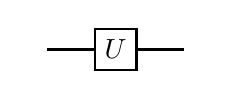
\begin{tikzpicture}[thick]
    %
    % `operator' will only be used by Hadamard (H) gates here.
    % `phase' is used for controlled phase gates (dots).
    % `surround' is used for the background box.
    \tikzstyle{operator} = [draw,fill=white,minimum size=1.5em] 
    \tikzstyle{phase} = [fill,shape=circle,minimum size=5pt,inner sep=0pt]
    \tikzstyle{surround} = [fill=blue!10,thick,draw=black,rounded corners=2mm]
    
    \node at (0,0) (begin1) {};
    \node[operator] (op1) at (1,0) {$U$} edge [-] (begin1);
    \node at (2,0) (end1) {} edge [-] (op1);
\end{tikzpicture}
\end{center}

where the ``input'' edge is to the left of operation $U$, and the ``output'' edge is to the right of $U$. In other words, we assume that operations are ordered from left
to right. For example,

\begin{center}
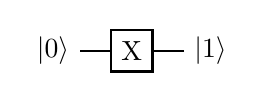
\begin{tikzpicture}[thick]
    %
    % `operator' will only be used by Hadamard (H) gates here.
    % `phase' is used for controlled phase gates (dots).
    % `surround' is used for the background box.
    \tikzstyle{operator} = [draw,fill=white,minimum size=1.5em] 
    \tikzstyle{phase} = [fill,shape=circle,minimum size=5pt,inner sep=0pt]
    \tikzstyle{surround} = [fill=blue!10,thick,draw=black,rounded corners=2mm]
    
    \node at (0,0) (begin1) {$\ket{0}$};
    \node[operator] (op1) at (1,0) {X} edge [-] (begin1);
    \node at (2,0) (end1) {$\ket{1}$} edge [-] (op1);
\end{tikzpicture}
\end{center}

Shows a circuit with input qubit $\ket{0}$ that is acted on by $X$, which has the effect of flipping the qubit to $\ket{1}$.

Also, a sequence of operations acting on a qubit may be combined into one, as is shown below.

\begin{center}
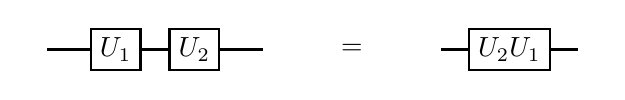
\begin{tikzpicture}[thick]
    %
    % `operator' will only be used by Hadamard (H) gates here.
    % `phase' is used for controlled phase gates (dots).
    % `surround' is used for the background box.
    \tikzstyle{operator} = [draw,fill=white,minimum size=1.5em] 
    \tikzstyle{phase} = [fill,shape=circle,minimum size=5pt,inner sep=0pt]
    \tikzstyle{surround} = [fill=blue!10,thick,draw=black,rounded corners=2mm]
    
    \node at (0,0) (begin1) {};
    \node[operator] (op1) at (1,0) {$U_1$} edge [-] (begin1);
    \node[operator] (op2) at (2,0) {$U_2$} edge [-] (op1);
    \node at (3,0) (end1) {} edge [-] (op2);
    \node at (4,0) (begin1) {$=$};
    \node at (5,0) (begin2) {};
    \node[operator] (op3) at (6,0) {$U_2U_1$} edge [-] (begin2);
    \node at (7,0) (end1) {} edge [-] (op3);
\end{tikzpicture}
\end{center}

Circuit operations may also occur in parallel with each operating on a different qubit. Parallel operations are considered independent in the sense that
the result of two parallel operations $A$ and $B$ is $A\otimes B$ as is shown below.

\begin{center}
\begin{tikzpicture}[thick]
    %
    % `operator' will only be used by Hadamard (H) gates here.
    % `phase' is used for controlled phase gates (dots).
    % `surround' is used for the background box.
    \tikzstyle{operator} = [draw,fill=white,minimum size=1.5em] 
    \tikzstyle{phase} = [fill,shape=circle,minimum size=5pt,inner sep=0pt]
    \tikzstyle{surround} = [fill=blue!10,thick,draw=black,rounded corners=2mm]
    
    \node at (0,0) (begin1) {};
    \node[operator] (op1) at (1,0) {$A$} edge [-] (begin1);
    \node at (2,0) (end1) {} edge [-] (op1);
    
     \node at (3,-1)  {$=$};
      \node at (4,-1)  {$A\otimes B$};
    
    \node at (0,-2) (begin2) {};
    \node[operator] (op2) at (1,-2) {$B$} edge [-] (begin2);
    \node at (2,-2) (end2) {} edge [-] (op2);
\end{tikzpicture}
\end{center}

By Theorem 5, the following two parallel circuits are identical

\begin{center}
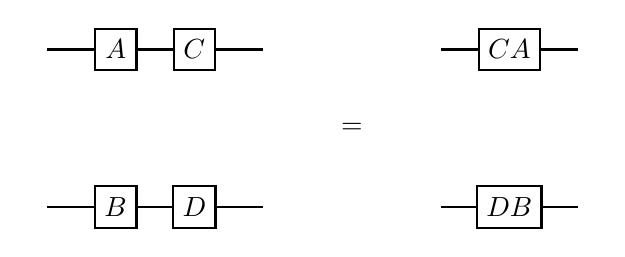
\begin{tikzpicture}[thick]
    %
    % `operator' will only be used by Hadamard (H) gates here.
    % `phase' is used for controlled phase gates (dots).
    % `surround' is used for the background box.
    \tikzstyle{operator} = [draw,fill=white,minimum size=1.5em] 
    \tikzstyle{phase} = [fill,shape=circle,minimum size=5pt,inner sep=0pt]
    \tikzstyle{surround} = [fill=blue!10,thick,draw=black,rounded corners=2mm]
    
    \node at (0,0) (begin1) {};
    \node[operator] (op1) at (1,0) {$A$} edge [-] (begin1);
    \node[operator] (op3) at (2,0) {$C$} edge [-] (op1);
    \node at (3,0) (end1) {} edge [-] (op3);
    
     \node at (4,-1)  {$=$};
     %\node at (4,-1)  {$A\otimes B$};
    
    \node at (0,-2) (begin2) {};
    \node[operator] (op2) at (1,-2) {$B$} edge [-] (begin2);
    \node[operator] (op4) at (2,-2) {$D$} edge [-] (op2);
    \node at (3,-2) (end2) {} edge [-] (op4);
    
    \node at (5,0) (begin10) {};
    \node[operator] (op10) at (6,0) {$CA$} edge [-] (begin10);
    \node at (7,0) (end10) {} edge [-] (op10);
    
    \node at (5,-2) (begin20) {};
    \node[operator] (op20) at (6,-2) {$DB$} edge [-] (begin20);
    \node at (7,-2) (end20) {} edge [-] (op20);
\end{tikzpicture}
\end{center}

since $(C\otimes D)(A\otimes B) = (CA)\otimes (DB)$.

The circuits presented so far cannot create dependency between two qubits. A fundamental way to create dependency
between two qubits is allowing one to act as a \textbf{control bit} for the other, meaning that an operation is performed on the second qubit
provided the first qubit is in the 1 state. A common example of this that is often used in this lecture occurs when the control bit has the effect of 
flipping the value of the second bit. We refer to this as \textbf{controlled not}, or c-NOT. Mathematically we have 
\[\ket{ab}\rightarrow \ket{a(b\oplus a)}\]
which may be achieved with the matrix

\[
\left(\begin{array}{cccc}
1 & 0 & & \\
0 &  1 & &  \\
& & 0 & 1\\
& & 1 & 0\\
\end{array}\right)
=
\left(\begin{array}{c|c}
I & \\
\hline
 &  X \\
\end{array}\right)
\]

\newpage
Diagrammatically, controlled not is represented as 

\begin{center}
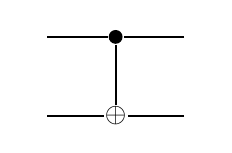
\begin{tikzpicture}[thick]
    %
    % `operator' will only be used by Hadamard (H) gates here.
    % `phase' is used for controlled phase gates (dots).
    % `surround' is used for the background box.
    \tikzstyle{operator} = [draw,fill=white,minimum size=1.5em] 
    \tikzstyle{phase} = [fill,shape=circle,minimum size=5pt,inner sep=0pt]
    \tikzstyle{surround} = [fill=blue!10,thick,draw=black,rounded corners=2mm]
    \tikzstyle{symbol} = [minimum size=5pt,inner sep=0pt]
    
    \node at (0,0) (begin1) {};
    \node[phase] (op1) at (1,0) {} edge [-] (begin1);
    \node at (2,0) (end1) {} edge [-] (op1);
    
    \node at (0,-1) (begin2) {};
    \node[symbol](op2) at (1,-1) {$\oplus$} edge [-] (begin2);
    \node at (2,-1) (end2) {} edge [-] (op2);
    \draw[-] (op1) -- (op2);
\end{tikzpicture}
\end{center}


More generally, a \textbf{controlled-U} gate, denoted c-U, is one whose matrix corresponds with 
\[
\left(\begin{array}{c|c}
I & \\
\hline
 &  U \\
\end{array}\right)
\]

and is written diagrammatically as 


\begin{center}
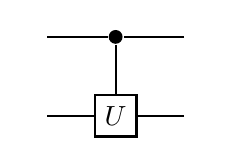
\begin{tikzpicture}[thick]
    %
    % `operator' will only be used by Hadamard (H) gates here.
    % `phase' is used for controlled phase gates (dots).
    % `surround' is used for the background box.
    \tikzstyle{operator} = [draw,fill=white,minimum size=1.5em] 
    \tikzstyle{phase} = [fill,shape=circle,minimum size=5pt,inner sep=0pt]
    \tikzstyle{surround} = [fill=blue!10,thick,draw=black,rounded corners=2mm]
    \tikzstyle{symbol} = [minimum size=5pt,inner sep=0pt]
    
    \node at (0,0) (begin1) {};
    \node[phase] (op1) at (1,0) {} edge [-] (begin1);
    \node at (2,0) (end1) {} edge [-] (op1);
    
    \node at (0,-1) (begin2) {};
    \node[operator](op2) at (1,-1) {$U$} edge [-] (begin2);
    \node at (2,-1) (end2) {} edge [-] (op2);
    \draw[-] (op1) -- (op2);
\end{tikzpicture}
\end{center}

In other words, $\ket{0a}\rightarrow\ket{0a}$, and $\ket{1a}\rightarrow\ket{1,Ua}$, where $Ua$ denotes $U\ket{a}$. 

\newpage
\textbf{Example 14.} Show that the following circuit outputs the uniform superposition of the numbers (i.e. basis states) $0,1,2,3$.

\begin{center}
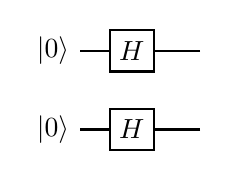
\begin{tikzpicture}[thick]
    %
    % `operator' will only be used by Hadamard (H) gates here.
    % `phase' is used for controlled phase gates (dots).
    % `surround' is used for the background box.
    \tikzstyle{operator} = [draw,fill=white,minimum size=1.5em] 
    \tikzstyle{phase} = [fill,shape=circle,minimum size=5pt,inner sep=0pt]
    \tikzstyle{surround} = [fill=blue!10,thick,draw=black,rounded corners=2mm]
    
    \node at (0,0) (begin1) {$\ket{0}$};
    \node[operator] (op1) at (1,0) {$H$} edge [-] (begin1);
    \node at (2,0) (end1) {} edge [-] (op1);
    
    
    
    \node at (0,-1) (begin2) {$\ket{0}$};
    \node[operator] (op2) at (1,-1) {$H$} edge [-] (begin2);
    \node at (2,-1) (end2) {} edge [-] (op2);
\end{tikzpicture}
\end{center}


\newpage
Another fundamental qubit operation is the \textbf{phase shift} gate 
\begin{center}
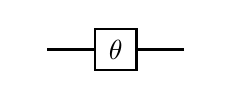
\begin{tikzpicture}[thick]
    %
    % `operator' will only be used by Hadamard (H) gates here.
    % `phase' is used for controlled phase gates (dots).
    % `surround' is used for the background box.
    \tikzstyle{operator} = [draw,fill=white,minimum size=1.5em] 
    \tikzstyle{phase} = [fill,shape=circle,minimum size=5pt,inner sep=0pt]
    \tikzstyle{surround} = [fill=blue!10,thick,draw=black,rounded corners=2mm]
    \tikzstyle{symbol} = [minimum size=5pt,inner sep=0pt]
    
    \node at (0,0) (begin1) {};
    \node[operator] (op1) at (1,0) {$\theta$} edge [-] (begin1);
    \node at (2,0) (end1) {} edge [-] (op1);
\end{tikzpicture}
\end{center}
whose associated matrix is 
\[
\left(\begin{array}{cc}
1 & 0 \\
0 &  e^{\theta i} \\
\end{array}\right)
\]

Recall that any single-qubit state can be written as the superposition $v_1\ket{0}+v_2\ket{1}$, where $v_1,v_2\in \mathbb{C}$, and
$|v_1|^2+|v_2|^2=1$. Thus, we may write $v_j=r_je^{\phi_j i}$, $j=0,1$, where $\phi_j$ is the phase of $\ket{j}$. 
However, given that we are usually interested in the \textit{relative phase difference} between $\ket{0}$ and $\ket{1}$, we may assume $\phi_0=0$.
Moreover, since $r_0^2 + r_1^2 = 1$, we may write $r_0=\cos\theta$ and $r_1=\sin\theta$ for some unique $\theta\in[0,2\pi)$. Thus the general 
form of a superimposed qubit is
\[\cos\theta\ket{0}+e^{\phi i}\sin\theta \ket{1}.\]

\textbf{Theorem 6.} The following quantum circuit is correct.

\begin{center}
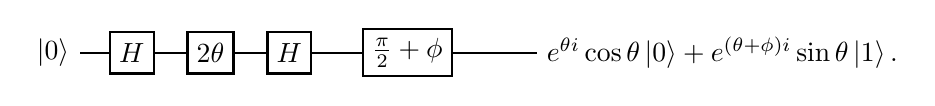
\begin{tikzpicture}[thick]
    %
    % `operator' will only be used by Hadamard (H) gates here.
    % `phase' is used for controlled phase gates (dots).
    % `surround' is used for the background box.
    \tikzstyle{operator} = [draw,fill=white,minimum size=1.5em] 
    \tikzstyle{phase} = [fill,shape=circle,minimum size=5pt,inner sep=0pt]
    \tikzstyle{surround} = [fill=blue!10,thick,draw=black,rounded corners=2mm]
    \tikzstyle{symbol} = [minimum size=5pt,inner sep=0pt]
    
    \node at (0,0) (begin1) {$\ket{0}$};
    \node[operator] (op1) at (1,0) {$H$} edge [-] (begin1);
    \node[operator] (op2) at (2,0) {$2\theta$} edge [-] (op1);
    \node[operator] (op3) at (3,0) {$H$} edge [-] (op2);
    \node[operator] (op4) at (4.5,0) {$\frac{\pi}{2}+\phi$} edge [-] (op3);
    \node at (8.5,0)  {$e^{\theta i}\cos\theta\ket{0}+e^{(\theta+\phi) i}\sin\theta \ket{1}\mbox{.}$} edge [-] (op4);
\end{tikzpicture}
\end{center}

\textbf{Proof of Theorem 6.} We have
\[H\ket{0} = \frac{1}{\sqrt{2}}\ket{0} + \frac{1}{\sqrt{2}}\ket{1},\]
And applying a $2\theta$-phase shift yields 
\[\frac{1}{\sqrt{2}}\ket{0} + \frac{e^{2\theta i}}{\sqrt{2}}\ket{1}.\]
Next, by linearity,
\[H(\frac{1}{\sqrt{2}}\ket{0} + \frac{e^{2\theta i}}{\sqrt{2}}\ket{1}) = \frac{1}{2}(1+e^{2\theta i})\ket{0} + \frac{1}{2}(1-e^{2\theta i})\ket{1}.\]
Finally, applying a $(\frac{\pi}{2}+\phi)$-phase shift yields
\[\frac{1}{2}(1+e^{2\theta i})\ket{0} + \frac{1}{2}(1-e^{2\theta i})e^{(\frac{\pi}{2}+\phi)i}\ket{1}=\]
\[\frac{1}{2}(1+\cos 2\theta + i\sin 2\theta)\ket{0} + \frac{1}{2}(1-\cos 2\theta - i\sin 2\theta)e^{\frac{\pi}{2}i}e^{\phi i}\ket{1}=\]
\[\frac{1}{2}(1+\cos^2\theta -\sin^2\theta + 2i\sin\theta \cos \theta)\ket{0} + \frac{1}{2}(1-\cos^2\theta +\sin^2\theta - 2i\sin \theta\cos\theta)i e^{\phi i}\ket{1}=\]
\[\frac{1}{2}(2\cos^2\theta  + 2i\sin\theta \cos\theta)\ket{0} + \frac{1}{2}(2\sin^2\theta i  + 2\sin \theta\cos\theta) e^{\phi i}\ket{1}=\]
\[\cos\theta(\cos\theta  + i\sin\theta)\ket{0} + \sin\theta(\sin\theta i  + \cos\theta) e^{\phi i}\ket{1}=\]
\[e^{\theta i}\cos\theta\ket{0} + \sin\theta e^{(\theta+\phi) i}\ket{1},\]
where we've used the following trigonometric identities.
\begin{enumerate}
\item $\sin 2\theta  = 2\sin\theta \cos\theta$
\item $\cos 2\theta  = \cos^2\theta - \sin^2\theta$
\item $\cos^2\theta + \sin^2\theta = 1$
\item $\cos\theta  + i\sin\theta = e^{\theta i}$
\end{enumerate}
\qed

Since \texttt{And}, \texttt{Not}, and \texttt{Or} gates can be used to compute any Boolean function, these three gates form a \textbf{universal set} of gates for computing Boolean functions.
Similarly, it can be shown that any $n$-qubit unitary transformation may be computed using $H$, c-NOT, and phase gates, and so collectively these gates form an infinite (since there are an infinite number of phases)  universal set for computing unitary transformations. Note however, if we only require approximating unitary transformations to any degree of accuracy, then the $H$ and c-V gates suffice to form a universal set, where
\[V=
\left(\begin{array}{cc}
1 & 0\\
0 &  i \\
\end{array}\right)
\]
is the $\frac{\pi}{2}$-phase shift.
For example, if $U$ is a unitary transformation, then, using a combination of $H$ and c-V gates, we may construct a transformation $U^{\prime}$ for which the length
$|U\ket{x}-U^{\prime}\ket{x}|$ can be made arbitrarily close to zero.

\subsection*{Logic and arithmetic circuits}
We now show how to use combinations of $H$ and $\mbox{c-}V$ gates in order to build controlled gates that behave like the Boolean logic gates
\texttt{AND}, \texttt{XOR}, and \texttt{NOT}. The idea is that the control qubit(s), and perhaps the target qubit, serves as input(s) to the gate, while the target qubit serves as output. From this perspective, 
and since c-NOT yields
\[\ket{ab}\rightarrow \ket{a(b\oplus a)},\]
we see that a c-NOT gate naturally computes  \texttt{XOR} since, if we view both control qubit $\ket{a}$ and target qubit $\ket{b}$ as inputs, 
then the target qubit is $\ket{a\oplus b}$. Moreover, for \texttt{NOT} only the control serves as input, while the target is initially set to $\ket{1}$, in which case
the target becomes $\ket{a\oplus b}=\ket{\overline{a}}$.

\newpage
\textbf{Theorem 7.} 

\begin{center}
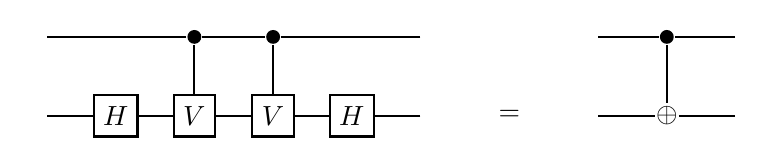
\begin{tikzpicture}[thick]
    %
    % `operator' will only be used by Hadamard (H) gates here.
    % `phase' is used for controlled phase gates (dots).
    % `surround' is used for the background box.
    \tikzstyle{operator} = [draw,fill=white,minimum size=1.5em] 
    \tikzstyle{phase} = [fill,shape=circle,minimum size=5pt,inner sep=0pt]
    \tikzstyle{surround} = [fill=blue!10,thick,draw=black,rounded corners=2mm]
    \tikzstyle{symbol} = [minimum size=8pt,inner sep=0pt]
    
    \node at (0,0) (begin1) {};
    \node[phase] (p1) at (2,0) {} edge [-] (begin1);
    \node[phase] (p2) at (3,0) {} edge [-] (p1);
    \node at (5,0) (end1) {} edge [-] (p2);
    
    \node at (0,-1) (begin2) {};
    \node[operator] (op1) at (1,-1) {$H$} edge [-] (begin2);
    \node[operator] (op2) at (2,-1) {$V$} edge [-] (op1);
    \node[operator] (op3) at (3,-1) {$V$} edge [-] (op2);
    \node[operator] (op4) at (4,-1) {$H$} edge [-] (op3);
    \node at (5,-1) (end2) {} edge [-] (op4);
    \draw[-] (p1) -- (op2);
    \draw[-] (p2) -- (op3);
    
     \node at (6,-1)  {$=$};
    
    \node at (7,0) (begin1) {};
    \node[phase] (pnot) at (8,0) {} edge [-] (begin1);
    \node at (9,0) (end1) {} edge [-] (pnot);
    
    \node at (7,-1) (begin3) {};
    \node[symbol](s1) at (8,-1) {$\oplus$} edge [-] (begin3);
    \node at (9,-1) (end3) {} edge [-] (s1);
    \draw[-] (pnot) -- (s1);
    
\end{tikzpicture}
\end{center}

\textbf{Proof of Theorem 7.} We show two different approaches to showing that the above circuits represent the same unitary transformation. 
In the first approach we show that both circuits yield the same unitary matrix. Indeed, the left circuit's unitary matrix is
\[
\left(\begin{array}{c|c}
H & \\
\hline
 &  H \\
\end{array}\right)
\left(\begin{array}{c|c}
I & \\
\hline
 &  V \\
\end{array}\right)
\left(\begin{array}{c|c}
I & \\
\hline
 &  V \\
\end{array}\right)
\left(\begin{array}{c|c}
H & \\
\hline
 &  H \\
\end{array}\right)
=
\left(\begin{array}{c|c}
(HIIH) & \\
\hline
 &  (HVVH) \\
\end{array}\right)
=
\left(\begin{array}{c|c}
I & \\
\hline
 &  X \\
\end{array}\right)
\]
which is the matrix for the right circuit.
It is left as an exercise to show that $HVVH=X$.

The second approach is to consider each of the possible cases of the input qubits $\ket{x}$ and $\ket{y}$, where $\ket{x}$ is the control and $\ket{y}$
is the target. If $\ket{x}=\ket{0}$ then the $V$ gates have no effect, and the transformation of $\ket{y}$ simplifies to $HH^{\dagger}=HH=I$, and so $\ket{y}$ does not change.

On the other hand, if $\ket{x}=\ket{1}$, then $\ket{y}$ is transformed by $HVVH=X$, which flips $\ket{y}$. Therefore, the left circuit is equivalent to c-not. \qed

To obtain an \texttt{AND} gate we use the concept of a controlled gate having two control inputs $\ket{a}$ and $\ket{b}$, and a target input $\ket{c}$ whose value
is flipped in case both $\ket{a}=\ket{b}=\ket{1}$. Thus, the transformation may be written as
\[\ket{abc}\rightarrow\ket{ab(c\oplus(a\wedge b))}.\]
Moreover, setting $\ket{c}=\ket{0}$ yields
\[\ket{ab0}\rightarrow\ket{ab(a\wedge b)},\]
and so the third input qubit becomes \texttt{AND} of control inputs $\ket{a}$ and $\ket{b}$. This gate is referred to as a $c^2\mbox{-not}$, or the
\textbf{Toffoli gate}, and  is diagramatically 
represented as 

\begin{center}
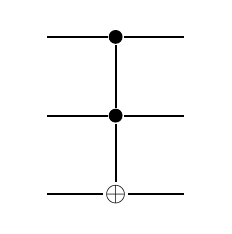
\begin{tikzpicture}[thick]
    %
    % `operator' will only be used by Hadamard (H) gates here.
    % `phase' is used for controlled phase gates (dots).
    % `surround' is used for the background box.
    \tikzstyle{operator} = [draw,fill=white,minimum size=1.5em] 
    \tikzstyle{phase} = [fill,shape=circle,minimum size=5pt,inner sep=0pt]
    \tikzstyle{surround} = [fill=blue!10,thick,draw=black,rounded corners=2mm]
    \tikzstyle{symbol} = [minimum size=8pt,inner sep=0pt]
    
    \node at (0,0) (begin1) {};
    \node[phase] (p1) at (1,0) {} edge [-] (begin1);
    \node at (2,0) (end1) {} edge [-] (p1);
    
    \node at (0,-1) (begin2) {};
    \node[phase] (p2) at (1,-1) {} edge [-] (begin2);
    \node at (2,-1) (end2) {} edge [-] (p2);
    
    \node at (0,-2) (begin3) {};
    \node[symbol](s1) at (1,-2) {$\oplus$} edge [-] (begin3);
    \node at (2,-2) (end3) {} edge [-] (s1);
    \draw[-] (p1) -- (p2);
    \draw[-] (p2) -- (s1);
    
\end{tikzpicture}
\end{center}

\newpage
\textbf{Example 15.} Verify that the Toffoli gate can be realized by the following circuit.


\begin{center}
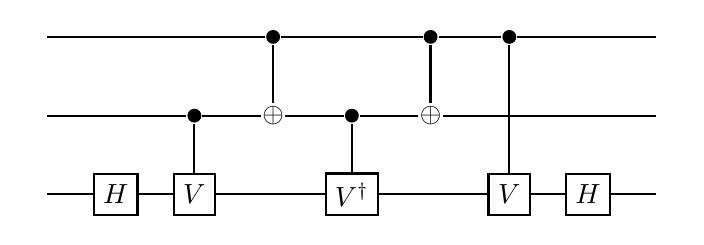
\begin{tikzpicture}[thick]
    %
    % `operator' will only be used by Hadamard (H) gates here.
    % `phase' is used for controlled phase gates (dots).
    % `surround' is used for the background box.
    \tikzstyle{operator} = [draw,fill=white,minimum size=1.5em] 
    \tikzstyle{phase} = [fill,shape=circle,minimum size=5pt,inner sep=0pt]
    \tikzstyle{surround} = [fill=blue!10,thick,draw=black,rounded corners=2mm]
    \tikzstyle{symbol} = [minimum size=8pt,inner sep=0pt]
    
    \node at (0,0) (begin1) {};
    \node[phase] (p1) at (3,0) {} edge [-] (begin1);
    \node[phase] (p2) at (5,0) {} edge [-] (p1);
     \node[phase] (p3) at (6,0) {} edge [-] (p2);
    \node at (8,0) (end1) {} edge [-] (p3);
    
    \node at (0,-1) (begin2) {};
    \node[phase] (pp1) at (2,-1) {} edge [-] (begin2);
    \node[symbol](s1) at (3,-1) {$\oplus$} edge [-] (pp1);
    \node[phase] (pp2) at (4,-1) {} edge [-] (s1);
    \node[symbol](s2) at (5,-1) {$\oplus$} edge [-] (pp2);
    \node at (8,-1) (end2) {} edge [-] (s2);
    
    \node at (0,-2) (begin3) {};
    \node[operator] (op1) at (1,-2) {$H$} edge [-] (begin3);
    \node[operator] (op2) at (2,-2) {$V$} edge [-] (op1);
    \node[operator] (op3) at (4,-2) {$V^{\dagger}$} edge [-] (op2);
    \node[operator] (op4) at (6,-2) {$V$} edge [-] (op3);
    \node[operator] (op5) at (7,-2) {$H$} edge [-] (op4);
    \node at (8,-2) (end3) {} edge [-] (op5);
    \draw[-] (pp1) -- (op2);
    \draw[-] (p1) -- (s1);
    \draw[-] (pp2) -- (op3);
    \draw[-] (p2) -- (s2);
    \draw[-] (p3) -- (op4);
    
\end{tikzpicture}
\end{center}

where
\[V^{\dagger}=
\left(\begin{array}{cc}
1 & 0\\
0 &  -i \\
\end{array}\right)
\]
is the inverse of $V$. Do this by considering all four possible control-input combinations. 

\newpage
Both the Toffoli and c-NOT gate may now be used to create a single-qubit adder as is shown above.

\begin{figure}
\begin{center}
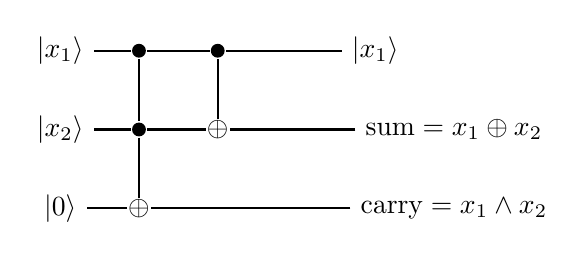
\begin{tikzpicture}[thick]
    %
    % `operator' will only be used by Hadamard (H) gates here.
    % `phase' is used for controlled phase gates (dots).
    % `surround' is used for the background box.
    \tikzstyle{operator} = [draw,fill=white,minimum size=1.5em] 
    \tikzstyle{phase} = [fill,shape=circle,minimum size=5pt,inner sep=0pt]
    \tikzstyle{surround} = [fill=blue!10,thick,draw=black,rounded corners=2mm]
    \tikzstyle{symbol} = [minimum size=5pt,inner sep=0pt]
    
    \node at (0,0) (begin1) {$\ket{x_1}$};
    \node[phase] (p1) at (1,0) {} edge [-] (begin1);
    \node[phase] (p2) at (2,0) {} edge [-] (p1);
    \node at (4,0) (end1) {$\ket{x_1}$} edge [-] (p2);

    \node at (0,-1) (begin2) {$\ket{x_2}$};
    \node[phase] (p3) at (1,-1) {} edge [-] (begin2);
    \node[symbol](s1) at (2,-1) {$\oplus$} edge [-] (p3);
    \node at (5,-1) (end2) {$\mbox{sum} = x_1\oplus x_2$} edge [-] (s1);
    
    \node at (0,-2) (begin3) {$\ket{0}$};
    \node[symbol](s2) at (1,-2) {$\oplus$} edge [-] (begin3);
    \node at (5,-2) (end3) {$\mbox{carry} = x_1\wedge x_2$} edge [-] (s2);
    \draw[-] (p1) -- (p3);
    \draw[-] (p3) -- (s2);
    \draw[-] (p2) -- (s1);
    
\end{tikzpicture}
\end{center}
\caption{Circuit for a single-qubit adder}
\end{figure}

\newpage
\section*{Quantum Information}

\textbf{Quantum information theory} studies the means for measuring, storing, and communicating qubits of information, and represents a generalization of classical information theory,
which studies similar issues in relation to classical bits of information. In this section we present two fundamental results from the theory: a method for
quantum teleportation, and the No-Cloning Theorem.

\subsection*{No-Cloning Theorem}

Given a quantum state $\ket{\psi}$, a \textbf{copy} of $\ket{\psi}$ is the quantum state vector $\ket{\psi}\otimes \ket{\psi}$, which implies that i) both state vectors that form
the tensor product have identical probability distributions (over the set of basis states) and ii) by Theorem 4, the measurement of one state vector is independent of the measurement
of the other. Notice that property ii) is essential, just as it is essential that whatever you do with your electronic copy of this lecture in no way affects my copy.

In order to make a copy of $\ket{\psi}$, we would need a quantum procedure, i.e. unitary matrix $U$, that inputs $\ket{\psi}$ and outputs $\ket{\psi}\otimes \ket{\psi}$.
But since $U$ is unitary, the input must be equal in dimension to the output, and so we must add another state vector $\ket{s}$ to our input, where $\ket{s}$ is some basis state,
and $\mbox{dim}(\ket{s})=\mbox{dim}(\ket{\psi})$. Note also that $\ket{s}$ is assumed independent of $\ket{\psi}$ (we may think of $\ket{s}$ as a built-in constant of our cloning
procedure). Hence, we must find a unitary matrix $U$, such that, for any arbitrary state vector $\ket{\psi}$, 
\[U(\ket{\psi}\otimes \ket{s}) = \ket{\psi}\otimes \ket{\psi}.\]

\textbf{No-Cloning Theorem.} There is no unitary matrix $U$ such that, for any arbitrary state vector $\ket{\psi}$, 
\[U(\ket{\psi}\otimes \ket{s}) = \ket{\psi}\otimes \ket{\psi}.\]

\newpage
\textbf{Proof of the No-Cloning Theorem.} Assume $U$ exists and consider two states $\ket{\psi}$ and $\ket{\phi}$ that we wish to copy.
Then we have 
\[U(\ket{\psi}\otimes \ket{s}) = \ket{\psi}\otimes \ket{\psi}\]
and
\[U(\ket{\phi}\otimes \ket{s}) = \ket{\phi}\otimes \ket{\phi}.\]
Moreover, by Corollary 2, we have
\[\langle \psi\otimes s | \phi\otimes s\rangle = \langle \psi | \phi\rangle \langle s|s\rangle = 
\langle \psi | \phi\rangle.\]
But since $U$ is unitary, we also have
\[\langle \psi\otimes s | \phi\otimes s\rangle = \langle U(\ket{\psi}\otimes \ket{s}) | U(\ket{\phi}\otimes \ket{s})\rangle = \]
\[ \langle \psi\otimes \psi | \phi\otimes \phi\rangle = \langle \psi | \phi\rangle\langle \psi | \phi\rangle =
(\langle \psi | \phi\rangle)^2,\]
where Corollary 2 is once again used, this time as the reason for the 2nd-to-last equality.
Thus, we may conclude that 
\[\langle \psi | \phi\rangle = (\langle \psi | \phi\rangle)^2,\]
which implies either $\langle \psi | \phi\rangle = 0$ or $\langle \psi | \phi\rangle = 1$. Now it is an exercise to show that, if 
$\langle \psi | \phi\rangle = 1$, then necessarily $\ket{\psi}=\ket{\phi}$. Thus, assuming $\ket{\psi}\not=\ket{\phi}$ we must have 
$\ket{\psi}$ orthogonal to $\ket{\phi}$, which contradicts the fact that there exist state vectors which are neither equal, nor orthogonal. For example,
$\ket{0}$ and $\ket{+}$ are two such vectors. \qed

\newpage
\subsection*{Quantum teleportation}

The problem of \textbf{quantum teleportation} is the problem of sending a qubit from one place to another. For example, suppose Alice lives in Los Angeles, Bob lives
Bob lives in Geneva, Switzerland, and Alice wants to send Bob her qubit $\ket{\psi}$, so that Bob can measure it. Note that $\ket{\psi}$ is superimposed, and so Alice cannot measure
it, since this would collapse it to a basis state. So Alice does not know the value of $\ket{\psi}$, and even if she did, theoretically it would take an infinite number of bits
to transmit the value, since $\ket{\psi}$ is a vector consisting of two complex numbers, each of which can have infinite precision. Two solve this problem, Alice and Bob must 
first get together at an earlier point in time (when $\ket{\psi}$ does not yet exist) and create the entangled two-qubit \textbf{Bell state} 
\[\frac{1}{\sqrt{2}}(\ket{00} + \ket{11}),\]
which can be accomplished with the following circuit.


\begin{center}
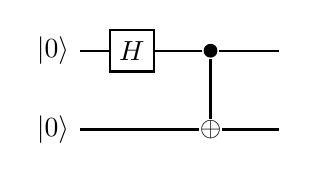
\begin{tikzpicture}[thick]
    %
    % `operator' will only be used by Hadamard (H) gates here.
    % `phase' is used for controlled phase gates (dots).
    % `surround' is used for the background box.
    \tikzstyle{operator} = [draw,fill=white,minimum size=1.5em] 
    \tikzstyle{phase} = [fill,shape=circle,minimum size=5pt,inner sep=0pt]
    \tikzstyle{surround} = [fill=blue!10,thick,draw=black,rounded corners=2mm]
    \tikzstyle{symbol} = [minimum size=5pt,inner sep=0pt]
    
    \node at (0,0) (begin1) {$\ket{0}$};
    \node[operator] (op1) at (1,0) {$H$} edge [-] (begin1);
    \node[phase] (p1) at (2,0) {} edge [-] (op1);
    \node at (3,0) (end1) {} edge [-] (p1);
    
    \node at (0,-1) (begin2) {$\ket{0}$};
    \node[symbol](cNot) at (2,-1) {$\oplus$} edge [-] (begin2);
    \node at (3,-1) (end2) {} edge [-] (cNot);
    \draw[-] (p1) -- (cNot);
    
\end{tikzpicture}
\end{center}

Notice that there are only two possible outputs to the circuit: $\ket{00}$ and $\ket{11}$, each occurring with equal likelihood. Once a Bell state is created, Alice and Bob each keep
one of the qubits, Alice eventually bringing hers to LA, and Bob bringing his to Geneva. A Bell state is also referred to as an \textbf{EPR pair}, where EPR stands for ``Einstein,
Podolsky, and Rosen'', whose 1935 paper used a Bell state to argue that, when Alice measures her qubit in LA, the value of Bob's qubit will be instantaneously known, implying that
information could travel faster than the speed of light. The current accepted theory resolves this apparent  paradox with the concept 
of a wave function that permeates all of space time, and that describes the superposition of possible quantum states.

\newpage
After creating the EPR pair $\ket{ab}$, weeks later Alice creates $\ket{\psi}$, and is now ready to transmit it to Bob. But rather than send $\ket{\psi}$ itself, Alice builds the 
following circuit, measures its output,
and sends the measurements to Bob in the form of two classical bits.

\begin{center}
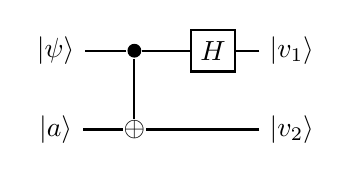
\begin{tikzpicture}[thick]
    %
    % `operator' will only be used by Hadamard (H) gates here.
    % `phase' is used for controlled phase gates (dots).
    % `surround' is used for the background box.
    \tikzstyle{operator} = [draw,fill=white,minimum size=1.5em] 
    \tikzstyle{phase} = [fill,shape=circle,minimum size=5pt,inner sep=0pt]
    \tikzstyle{surround} = [fill=blue!10,thick,draw=black,rounded corners=2mm]
    \tikzstyle{symbol} = [minimum size=5pt,inner sep=0pt]
    
    \node at (0,0) (begin1) {$\ket{\psi}$};
    \node[phase] (p1) at (1,0) {} edge [-] (begin1);
    \node[operator] (op1) at (2,0) {$H$} edge [-] (p1);
    \node at (3,0) (end1) {$\ket{v_1}$} edge [-] (op1);
    
    \node at (0,-1) (begin2) {$\ket{a}$};
    \node[symbol](cNot) at (1,-1) {$\oplus$} edge [-] (begin2);
    \node at (3,-1) (end2) {$\ket{v_2}$} edge [-] (cNot);
    \draw[-] (p1) -- (cNot);
    
\end{tikzpicture}
\end{center}

As shown above, the inputs to the circuit are $\ket{\psi}$ and $\ket{a}$, Alice's half of the EPR pair, and the output consists of qubits $\ket{v_1}$ and $\ket{v_2}$.

Now let $m_i\in\{0,1\}$, $i=1,2$, denote the outcome when Alice measures $\ket{v_i}$. Also, assume $\ket{\psi}=\alpha\ket{0}+\beta\ket{1}$.
Notice that, due to Alice's measurements, Bob's half $\ket{b}$ of the EPR pair $\ket{ab}$ is quite possibly no longer the same qubit that it was before Alice's measurements, in the sense
that it might not have the same probability distribution as before. As an example, suppose $\ket{\psi}=\ket{1}$. Then with certainty $\ket{a}$ was flipped by 
the c-NOT gate controlled by
$\ket{\psi}$, in which case measuring $\ket{b}$ will result in $1\oplus m_2$. In other words, after Alice's measurements, Bob's half of the EPR pair no longer has a 50-50 
probability distribution, but rather is equal to $1\oplus m_2$. In general, after receiving the $(m_1,m_2)$ 
pair, Bob's qubit now has the form $\ket{\hat{b}} = x\ket{0} + y\ket{1}$. Moreover, Bob is hoping that $x$ and $y$ depend linearly on $\alpha$ and $\beta$, so that he may then apply
a unitary transformation $U$ on $\ket{\hat{b}}$ to get $U\ket{\hat{b}}=\psi$, i.e., $U\ket{\hat{b}}=\alpha\ket{0}+\beta\ket{1}$.

To compute $x$ and $y$ conditioned on $(m_1,m_2)$, it helps to think of Alice's circuit as possessing a third input, namely $\ket{b}$ which is shown as follows.


\begin{center}
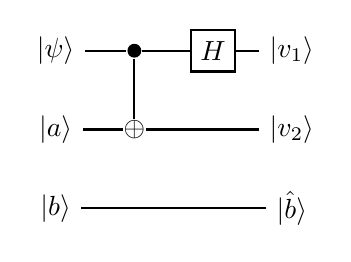
\begin{tikzpicture}[thick]
    %
    % `operator' will only be used by Hadamard (H) gates here.
    % `phase' is used for controlled phase gates (dots).
    % `surround' is used for the background box.
    \tikzstyle{operator} = [draw,fill=white,minimum size=1.5em] 
    \tikzstyle{phase} = [fill,shape=circle,minimum size=5pt,inner sep=0pt]
    \tikzstyle{surround} = [fill=blue!10,thick,draw=black,rounded corners=2mm]
    \tikzstyle{symbol} = [minimum size=5pt,inner sep=0pt]
    
    \node at (0,0) (begin1) {$\ket{\psi}$};
    \node[phase] (p1) at (1,0) {} edge [-] (begin1);
    \node[operator] (op1) at (2,0) {$H$} edge [-] (p1);
    \node at (3,0) (end1) {$\ket{v_1}$} edge [-] (op1);
    
    \node at (0,-1) (begin2) {$\ket{a}$};
    \node[symbol](cNot) at (1,-1) {$\oplus$} edge [-] (begin2);
    \node at (3,-1) (end2) {$\ket{v_2}$} edge [-] (cNot);
    \draw[-] (p1) -- (cNot);
    
    \node at (0,-2) (begin3) {$\ket{b}$};
    \node at (3,-2) (end3) {$\ket{\hat{b}}$} edge [-] (begin3);
    
\end{tikzpicture}
\end{center}

Notice that, although $\ket{b}$ does not pass through any gates, because it is entangled with $\ket{a}$, the output $\ket{\hat{b}}$ has the potential to be different
from $\ket{b}$. Our goal now is to compute $\ket{\hat{b}}$ on condition that $\ket{v_1}$ and $\ket{v_2}$ have been measured  as $(m_1,m_2)$.

The key insight to computing $\ket{\hat{b}}$ conditioned on $(m_1,m_2)$ lies in first considering the above circuit minus the Hadamard gate as shown below.

\begin{center}
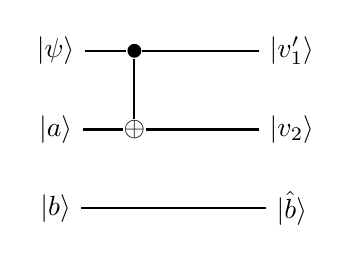
\begin{tikzpicture}[thick]
    %
    % `operator' will only be used by Hadamard (H) gates here.
    % `phase' is used for controlled phase gates (dots).
    % `surround' is used for the background box.
    \tikzstyle{operator} = [draw,fill=white,minimum size=1.5em] 
    \tikzstyle{phase} = [fill,shape=circle,minimum size=5pt,inner sep=0pt]
    \tikzstyle{surround} = [fill=blue!10,thick,draw=black,rounded corners=2mm]
    \tikzstyle{symbol} = [minimum size=5pt,inner sep=0pt]
    
    \node at (0,0) (begin1) {$\ket{\psi}$};
    \node[phase] (p1) at (1,0) {} edge [-] (begin1);
   % \node[operator] (op1) at (2,0) {$H$} edge [-] (p1);
    \node at (3,0) (end1) {$\ket{v_1^{\prime}}$} edge [-] (p1);
    
    \node at (0,-1) (begin2) {$\ket{a}$};
    \node[symbol](cNot) at (1,-1) {$\oplus$} edge [-] (begin2);
    \node at (3,-1) (end2) {$\ket{v_2}$} edge [-] (cNot);
    \draw[-] (p1) -- (cNot);
    
    \node at (0,-2) (begin3) {$\ket{b}$};
    \node at (3,-2) (end3) {$\ket{\hat{b}}$} edge [-] (begin3);
    
\end{tikzpicture}
\end{center}

With the help of the c-NOT unitary matrix, one can verify that this circuit has output
\[\frac{1}{\sqrt{2}}[\alpha\ket{0}(\ket{00} + \ket{11}) + \beta\ket{1}(\ket{10}+\ket{01})].\]
To avoid confusion, note that, e.g., $\ket{0}(\ket{00} + \ket{11})$ is shorthand for $\ket{0}\otimes (\ket{00} + \ket{11})$.
Furthermore, notice that the output to Alice's circuit can be obtained from the above circuit output by feeding the latter into 
$H\otimes I_4$, and so Alice's circuit has the output of 
\[(H\otimes I_4)(\frac{1}{\sqrt{2}}[\alpha\ket{0}(\ket{00} + \ket{11}) + \beta\ket{1}(\ket{10}+\ket{01})]) = \]
\[\frac{1}{2}[\alpha (\ket{0} +\ket{1}) (\ket{00} + \ket{11}) + \beta (\ket{0}-\ket{1}) (\ket{10} + \ket{01})] = \]
\[\frac{1}{2}[\alpha\ket{000}+\alpha\ket{011} + \alpha\ket{100}+\alpha\ket{111} +\]
\[\beta\ket{010} + \beta\ket{001} - \beta\ket{110} - \beta\ket{101}].\]
Finally, if we group the above terms with respect to the values of the first two qubits (which are the outputs to Alice's circuit), followed by factoring out those two 
qubits, we get that the above sum is equal to the sum of these groups:
\[\frac{1}{2}[\]
\[\ket{00}(\alpha\ket{0} + \beta\ket{1}) + \]
\[\ket{01}(\beta\ket{0} + \alpha\ket{1}) + \]
\[\ket{10}(\alpha\ket{0} - \beta\ket{1}) + \]
\[\ket{11}(-\beta\ket{0} + \alpha\ket{1})].\]
This is exactly what Bob is looking for. For example, suppose Alice sends Bob $(0,0)$. Then the remaining uncertainty in Alice's circuit (the one that includes $\ket{b}$ as input)
lies with the output $\ket{\hat{b}}=\alpha\ket{0} + \beta\ket{1} = \ket{\psi}$. In other words, after receiving Alice's bits, Bob's qubit has a distribution that is equal to that
of $\ket{\psi}$, and so to measure $\ket{\psi}$ Bob simply measures $\ket{\hat{b}}$. However, for the other three cases of what Alice may send, Bob must first multiply 
$\ket{\hat{b}}$ with an appropriate unitary matrix $U$ in order to obtain a qubit equal to $\ket{\psi}$.

\newpage
\textbf{Example 16.} For the other three cases, provide the $U$ matrix that Bob needs in order to transform $\ket{\hat{b}}$ to $\ket{\psi}$.






\newpage
One aspect of the solution to the quantum teleportation problem that may seem somewhat mysterious, if not magical, is how the $\alpha$ and $\beta$ components of $\ket{\psi}$ 
were taken away from the first output, $\ket{\psi}$, and given to the third output $\ket{\hat{b}}$. This is perfectly legal since, if $c$ is a complex scalar, then
\[c(\ket{u}\otimes\ket{v}) = \ket{cu}\otimes\ket{v} = \ket{u}\otimes\ket{cv}.\]
This is a wonderful example of how a mathematical model can be used to discover facts about the physical world!
















\newpage
\section*{Quantum Algorithms}

There are two aspects of quantum computing that provide an advantage over classical computation. 

\begin{enumerate}
\item A quantum state may be a superposition of basis states.
\item Superimposed states may be strategically added so that desirable states (i.e. ones corresponding to solutions) are in phase, while undesirable states 
are out of phase. This latter phenomenon is referred to as \textbf{interference}. This results in a superimposed state for which desired states have probability equal to or close to 
unity.
\end{enumerate}

In this section we demonstrate how to use these advantages in order to develop quantum algorithms that are more efficient than their classical counterparts. 
Here, a quantum algorithm for solving a problem is represented as a \textbf{uniform circuit family}, meaning an algorithm for constructing a quantum
circuit  $C_n$ that computes the solution to any problem instance having some fixed number $n$ of qubits. The  algorithm thus implies a family of circuits, since, for each specific
 value of
$n$, the algorithm describes how to construct a concrete circuit $C_n$, $n=0,1,\ldots$. Moreover, the family is said to be uniform, since the circuits are all related via a single
finite program $P$ for which the output of $P(i)$ is the circuit $C_i$, $i=0,1,\ldots$.  We may even think of $P$ as a URM program. In this case
 $P(i)=y$ represents the encoding of
circuit $C_i$. 

\newpage
\textbf{Example 16.} Consider the problem of adding two $n$-bit nonnegative integers $x=x_0x_1\cdots x_{n-1}$ and $y=y_0y_1\cdots y_{n-1}$. 
The following is an algorithm that describes how to construct a
(either classical or quantum) circuit
$C_n$ that computes $x+y$. To begin, recursively co-define carry bits $c_0,c_1,\ldots,c_{n}$, and sum bits $s_0,\ldots,s_{n}$, where 
\[c_0 = 0, \mbox{  } s_0 = x_0\oplus y_0,\]
\[c_i = (x_{i-1}\wedge y_{i-1}) \vee (c_{i-1}\wedge (x_{i-1}\vee y_{i-1})) \mbox{ if } 1\leq i\leq n,\]
and
\[s_i = c_{i} \oplus x_i \oplus y_i \mbox{ if } 1\leq i\leq n-1,\]
and
\[s_n = c_n.\]
Then the circuit output is then $s=s_0\cdots s_n$, and the circuit can be constructed by replacing $\wedge$, $\vee$, and $\oplus$ in the above equations with there
respective gates (either classical or quantum). Notice how the above equations do not represent any one particular circuit. Indeed, a concrete circuit may only be constructed once 
a specific value of $n$ is provided.
\qed

\subsection*{The Signed basis}

The \textbf{signed basis} represents
an important orthonormal basis for quantum computing, and is obtained by applying a Hadamard transformation to each of the 
basis state vectors. 

For example, one can verify that the single-qubit signed basis 
\[\{H\ket{0},H\ket{1}\} = \{\frac{1}{\sqrt{2}}(\ket{0}+\ket{1}),\frac{1}{\sqrt{2}}(\ket{0}-\ket{1})\}.\]
is an orthonormal set of vectors. 

In what follows we use the convention that $H_n$ denotes the $n$-fold tensor product $H\otimes H\otimes\cdots \otimes H$.
Then the two-qubit signed basis is (by using Corollarys 1 and 2 after Theorem 5)
\[\{H_2\ket{00},H_2\ket{01}, H_2\ket{10}, H_2\ket{11}\} =\]
\[ \{H\ket{0}\otimes H\ket{0}, H\ket{0}\otimes H\ket{1},
H\ket{1}\otimes H\ket{0},H\ket{1}\otimes H\ket{1}\} =\]
\[\{\frac{1}{2}(\ket{00} + \ket{01} + \ket{10} + \ket{11}), \frac{1}{2}(\ket{00} - \ket{01} + \ket{10} - \ket{11}),\]
\[\mbox{    }\frac{1}{2}(\ket{00} + \ket{01} - \ket{10} - \ket{11}), \frac{1}{2}(\ket{00} - \ket{01} - \ket{10} + \ket{11})\}\]

Notice that every vector in the signed basis has a  uniform distribution, meaning that, upon collapsing the wave function,
 each basis state vector has an equal probability of being observed.
 
There exist two useful conventions for writing signed basis vectors. The first uses ket notation, along with the symbols $+$ and $-$.
For example, $H\ket{0}=\ket{+}$, $H\ket{1}=\ket{-}$, $H_2\ket{01}=\ket{+-}$, etc..

The second convention is to write the 1 and -1 coefficients of the vector when written as a linear combination of the basis state vectors.
For example,  since 
\[ H_2\ket{01} =  \frac{1}{2}(\ket{00} - \ket{01} + \ket{10} - \ket{11}),\]
we may write it as $(1,-1,1,-1)$, while omitting the normalization factor of $1/2$. We call this the \textbf{signature} of the signed basis vector.

The following theorem establishes that the signed basis vectors always form an orthonormal basis.

\textbf{Theorem 8.} Let $\ket{0\cdots 0},\ldots,\ket{1\cdots 1}$ denote the $2^{n}$ $n$-qubit basis state vectors. Then 
\[H_n\ket{0\cdots 0}, \ldots, H_n\ket{1\cdots 1}\]
is an orthonormal basis for the $2^n$-dimensional $n$-qubit state space.

\textbf{Proof of Theorem 8.} First note that, since $H_n$ is unitary (see exercises!), then $H\ket{u}=\vec{0}$ implies that $\ket{u}=\vec{0}$.
Hence, 
\[H_n\ket{0\cdots 0}, \ldots, H_n\ket{1\cdots 1}\]
are all nonzero vectors. Moreover, if $\ket{u}=\ket{u_1\cdots u_n}$, and $\ket{v}=\ket{v_1\cdots v_n}$ are two basis state vectors, then
\[\langle H_n\ket{u}| H_n\ket{v}\rangle = \langle Hu_1\otimes\cdots\otimes Hu_n| Hv_1\otimes\cdots\otimes Hv_n\rangle=\]
\[\langle Hu_1|Hv_1\rangle\cdots \langle Hu_n|Hv_n\rangle,\]
where the first equality is due to Corollary 1, and the second is due to Corollary 2.
Moreover, notice that, since $H\ket{0}=\ket{+}$ and $H\ket{1}=\ket{-}$ are orthogonal, then we must
have 
\[\langle H\ket{u}| H\ket{v}\rangle = 0\]
iff $\ket{u}\not=\ket{v}$ and 
\[\langle H_n\ket{u}| H_n\ket{v}\rangle = 1\]
iff $\ket{u}=\ket{v}$.
Therefore, since the set of vectors
\[\{H_n\ket{0\cdots 0}, \ldots, H_n\ket{1\cdots 1}\}\]
satisfies properties i) and ii) of an orthonormal basis, and there are $2^n$ vectors, then this set 
is an orthonormal basis for the $n$-qubit state space.\qed

The following additional facts about signed basis vectors will prove useful.

\begin{enumerate}
\item Since $H_n$ is its own inverse, applying $H_n$ to any signed basis vector $\ket{v}$ will map that vector back to the 
basis state vector $\ket{u}$ for which $H_n\ket{u}=\ket{v}$. In other words $H_nH_n\ket{u}=\ket{u}$.

\item Let $\ket{y}=H_n\ket{u}$ be a signed basis vector. Then 
\[\ket{y}=\frac{1}{2^{n/2}}\sum_{x}c_x\ket{x},\]
where $\mbox{domain}(x)=\{0,1,\ldots,2^{n-1}\}$, and $c_x = (-1)^{x\cdot u}$, where 
 $x\cdot u$ denotes the dot product between the basis-state vectors $\ket{x}$ and $\ket{u}$.
\end{enumerate}



 






\newpage
\subsection*{Deutsch's problem}

Consider a unary Boolean function $f:\{0,1\}\rightarrow\{0,1\}$. Deutsch's problem is to compute $f(0)\oplus f(1)$. In what follows, we represent $f$ as the two-bit string
$ab$, where $f(0)=a$ and $f(1)=b$. Now, if $f$ were realized by a classical Boolean circuit, then
we would requuire two circuit evaluations to obtain $f(0)\oplus f(1)$, namely $f(0)$ followed by $f(1)$. On the other hand, if $f$ is realized by a quantum circuit,
then we demonstrate how to obtain 
$f(0)\oplus f(1)$ via a \textit{single} circuit evaluation.

The first step is to define the two-qubit unitary operation 
\[U_f\ket{xy} = \ket{x,y\oplus f(x)}.\]

To see that $U_f$ is unitary, imagine that only an oracle knows how to compute $f(x)$ and that she is to provide us a $U_f$ gate for our quantum circuit. Moreover
the $U_f$ is only to be evaluated once. As an example, suppose $f=10$. Then the oracle must provide $U_f$ that satisfies 
\[U_f\ket{00} = \ket{01}, U_f\ket{01}=\ket{00}, U_f\ket{10} = \ket{10}, \mbox{ and } U_f\ket{11} = \ket{11}.\]
 This corresponds to the matrix
\[U_f = U_{10} =
\left(\begin{array}{cccc}
0 & 1 & 0 & 0\\
1 &  0 & 0 & 0 \\
0 &  0 & 1 & 0 \\
0 &  0 & 0 & 1 \\
\end{array}\right) =
\left(\begin{array}{c|c}
X & \\
\hline
 &  I \\
\end{array}\right)
\].

We leave it as an exercise to show that 
\[U_{00} = I, U_{01} = 
\left(\begin{array}{c|c}
I & \\
\hline
 &  X \\
\end{array}\right), \mbox{ and }
 U_{11} = 
\left(\begin{array}{c|c}
X & \\
\hline
 &  X \\
\end{array}\right).
\]
Of course, we do not know which of the four above transformations was provided by the oracle. In any case we compute $U_f\ket{+-}$.
The following table shows the possible ways that $U_f$ can transform the  $\ket{+-}$.
The fourth column shows the result of applying $H\otimes H$ to transforming $U_f\ket{+-}$ back to a basis state vector.
\[\begin{array}{|l|l|l|l|}
\hline
f & U_f &  u = U_f\ket{+-} & (H\otimes H)u\\
\hline
00 & U_{00} & (1,-1,1,-1) = \ket{+-} & \ket{01}\\
\hline
01 & U_{01} & (1,-1,-1,1) = \ket{--} & \ket{11}\\%\ket(11}\\
\hline
10 & U_{10} & (-1,1,1,-1) =  -1\ket{--} & -1\ket{11}\\
\hline
11 & U_{11} & (-1,1,-1,1) = -1\ket{+-} & -1\ket{01}\\
\hline
\end{array}
\]

One way to understand the above table is to first notice that the signature of $\ket{+-}$ is $(1,-1,1,-1)$. Also,
 notice that, if $f(x)=1$, then $U_f$ has the effect of swapping the signs of $\ket{x0}$ and $\ket{x1}$ in the signature
of $\ket{+-}$. For example, if $f=10$, then $f(0)=1$, and $U_f$ transforms the signature $(1,-1,1,-1)$ to that of $(-1,1,1,-1)$ by swapping the signs of
$\ket{00}$ with $\ket{01}$. This new signature may be factored to $-1(1,-1,-1,1)$ which is the negative signature of $\ket{--}$. 

\newpage
\textbf{Example 17.} Describe the sign swapping that takes place in both $U_{01}$ and $U_{11}$.


\newpage
\vspace{4.0in}
Thus, the desired circuit can now be described in the following three phases.
\begin{enumerate}
\item Compute $(H\otimes H)\ket{01}=\ket{+-}$ to obtain a uniform vector.
\item  Compute $u=U_f\ket{+-}$.
\item Compute $(H\otimes H)u$ to transform back to a basis state.
\end{enumerate}
Moreover, if $f$ has even (respectively, odd) parity, then the circuit outputs $\ket{01}$ (respectively, $\ket{11}$) along with a possible phase factor of -1, in the case
of $f=10$ and $f=11$. Notice that this phase factor does not affect the actual qubits that will be measured after the circuit has performed its evaluation. 
therefore, $f$ has even (respectively, odd) parity iff the first qubit is measured as $\ket{0}$ (respectively, $\ket{1}$).

\begin{figure}
\begin{center}
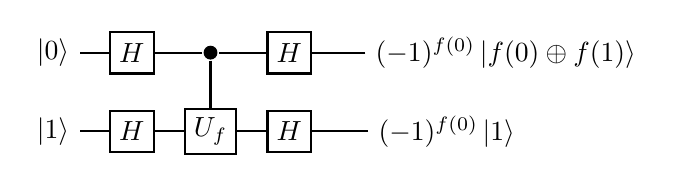
\begin{tikzpicture}[thick]
    %
    % `operator' will only be used by Hadamard (H) gates here.
    % `phase' is used for controlled phase gates (dots).
    % `surround' is used for the background box.
    \tikzstyle{operator} = [draw,fill=white,minimum size=1.5em] 
    \tikzstyle{phase} = [fill,shape=circle,minimum size=5pt,inner sep=0pt]
    \tikzstyle{surround} = [fill=blue!10,thick,draw=black,rounded corners=2mm]
    \tikzstyle{symbol} = [minimum size=5pt,inner sep=0pt]
    
    \node at (0,0) (begin1) {$\ket{0}$};
    \node[operator] (op1) at (1,0) {$H$} edge [-] (begin1);
    \node[phase] (p1) at (2,0) {} edge [-] (op1);
    \node[operator] (op2) at (3,0) {$H$} edge [-] (p1);
    \node at (5.75,0) (end1) {$(-1)^{f(0)}\ket{f(0)\oplus f(1)}$} edge [-] (op2);
    
    \node at (0,-1) (begin2) {$\ket{1}$};
    \node[operator] (op3) at (1,-1) {$H$} edge [-] (begin2);
    \node[operator](U) at (2,-1) {$U_f$} edge [-] (op3);
    \node[operator] (op4) at (3,-1) {$H$} edge [-] (U);
    \node at (5,-1) (end2) {$(-1)^{f(0)}\ket{1}$} edge [-] (op4);
    \draw[-] (p1) -- (U);
    
\end{tikzpicture}
\end{center}
\caption{Circuit solution to Deutsch's problem}
\end{figure}

\newpage
\subsection*{The Deutsch-Jozsa problem}

The Deutsch-Jozsa problem extends Deutsch's problem to the case where $f:\{0,1\}^n\rightarrow \{0,1\}$ is now an $n$-bit Boolean function. Moreover, we are told that $f$ 
is either a constant function, or is \textit{balanced} in that $f(x)=0$ for exactly half the inputs. The problem is to decide if $f$ is constant or balanced.

Classically, in the worst case we must query the oracle $2^{n-1}+1$ times
in order to decide if $f$ is constant. However, we may use a randomized algorithm that makes $r$ independent random queries to the oracle, and decides that $f$ is constant iff
all the query answers are identical. Furthermore, the probability that the algorithm returns the wrong answer equals the probability that all query answers are the same in the case
that $f$ is balanced. But this will happen with probability $2(1/2^r)=1/2^{r-1}$, and thus the probability of error declines exponentially in the number of queries.

As in the previous problem the first step is to define the $n+1$-qubit unitary operation 
\[U_f\ket{xy} = \ket{x,y\oplus f(x)},\]
where $x$ is assumed to have $n$ bits. As before, we may think of $U_f$ as a $2^{n+1}\times 2^{n+1}$ matrix such that, for basis state vector $\ket{xy}$,
\[U_f\ket{xy}=\left\{\begin{array}{ll} 
\ket{xy} & \mbox{ if } f(x) = 0 \\
\ket{x\overline{y}} & \mbox{ if } f(x) = 1 
\end{array}\right.
\]
Thus, the columns of $U_f$ are distinct basis state vectors, and hence $U_f$ is unitary (see Exercise~\ref{ex:unitary}).

Again, suppose the oracle prepares a quantum circuit for computing $U_f$. We show how to solve the Deutsch-Jozsa problem by performing a single evaluation of $U_f$ within
the following circuit.

\begin{center}
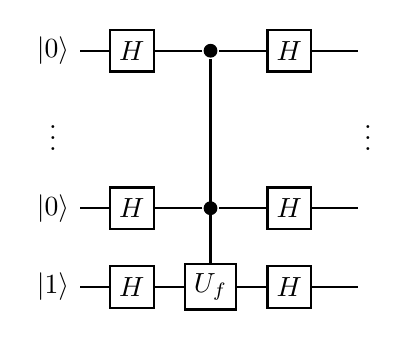
\begin{tikzpicture}[thick]
    %
    % `operator' will only be used by Hadamard (H) gates here.
    % `phase' is used for controlled phase gates (dots).
    % `surround' is used for the background box.
    \tikzstyle{operator} = [draw,fill=white,minimum size=1.5em] 
    \tikzstyle{phase} = [fill,shape=circle,minimum size=5pt,inner sep=0pt]
    \tikzstyle{surround} = [fill=blue!10,thick,draw=black,rounded corners=2mm]
    \tikzstyle{symbol} = [minimum size=5pt,inner sep=0pt]
    
    \node at (0,0) (begin1) {$\ket{0}$};
    \node[operator] (op1) at (1,0) {$H$} edge [-] (begin1);
    \node[phase] (p1) at (2,0) {} edge [-] (op1);
    \node[operator] (op2) at (3,0) {$H$} edge [-] (p1);
    \node at (4,0) (end1) {} edge [-] (op2);
    
    \node at (0,-1) () {$\vdots$};
    \node at (4,-1) () {$\vdots$};
    
    \node at (0,-2) (begin10) {$\ket{0}$};
    \node[operator] (op10) at (1,-2) {$H$} edge [-] (begin10);
    \node[phase] (p10) at (2,-2) {} edge [-] (op10);
    \node[operator] (op20) at (3,-2) {$H$} edge [-] (p10);
    \node at (4,-2) (end10) {} edge [-] (op20);
    
    \node at (0,-3) (begin2) {$\ket{1}$};
    \node[operator] (op3) at (1,-3) {$H$} edge [-] (begin2);
    \node[operator](U) at (2,-3) {$U_f$} edge [-] (op3);
    \node[operator] (op4) at (3,-3) {$H$} edge [-] (U);
    \node at (4,-3) (end2) {} edge [-] (op4);
    \draw[-] (p1) -- (U);
    
\end{tikzpicture}
\end{center}
 

\textbf{Theorem 9.} If $f$ is a constant, then the output of the Deutsch-Jozsa circuit is either $\ket{0\cdots 01}$ or $-1\ket{0\cdots 01}$. 
On the other hand, if $f$ is balanced, then with probability zero  $\ket{0\cdots 01}$ or 
$-1\ket{0\cdots 01}$ will be observed.


\newpage
\textbf{Proof of Theorem 9.} First note that the application of $H_{n+1}$ on input $\ket{0\cdots 01}$ produces the output $\ket{+\cdots +-}$. 
Moreover, 
\[\ket{+\cdots +-}= \sum_{x,y}(-1)^{(xy)\cdot (0\cdots 01)}\ket{xy} = \sum_{x,y}(-1)^y\ket{xy},\]
where $x\in\{0,1\}^n$ and $y\in\{0,1\}$. 

Now consider how $U_f$ acts on a single term $(-1)^y\ket{xy}$. There are four cases which are summarized in the following table.

\begin{tabular}{|l|l|l|}
\hline
\textbf{Constant function $f$} & \textbf{Value of $(-1)^y\ket{xy}$} & $U_f(-1)^y\ket{xy}$\\
\hline
$f(x) = 0$ & $\ket{x0}$ & $\ket{x0}$ \\
\hline
$f(x) = 0$ & $-\ket{x1}$ & $-\ket{x1}$ \\
\hline
$f(x) = 1$ & $\ket{x0}$ & $\ket{x1}$ \\
\hline
$f(x) = 1$ & $-\ket{x1}$ & $-\ket{x0}$ \\
\hline
\end{tabular}

Notice that, in the first two cases, i.e. $f(x)=0$, $U_f$ is the identity transformation, and so 
\[U_f\ket{+\cdots +-} = U_f(\sum_{x,y}(-1)^y\ket{xy}) = \sum_{x,y}(-1)^y\ket{xy} = \ket{+\cdots +-}.\]
On the other hand, when $f(x)=1$, the sign of each term in $\underset{x,y}{\sum}(-1)^y\ket{xy}$ gets changed, i.e.
\[U_f\ket{+\cdots +-} = U_f(\sum_{x,y}(-1)^y\ket{xy}) = -\sum_{x,y}(-1)^y\ket{xy} = -\ket{+\cdots +-}.\]
Hence, we can combine these two transformations into the single rule
\[U_f\ket{+\cdots +-} = U_f(\sum_{x,y}(-1)^y\ket{xy}) = (-1)^{f(x)}\sum_{x,y}(-1)^y\ket{xy}=(-1)^{f(x)} \ket{+\cdots +-}.\]

The final step of the circuit is to apply $H_{n+1}$ to $(-1)^{f(x)} \ket{+\cdots +-}$. Here we use the fact that, since $H$ is its own inverse, so is
$H_{n+1}$, and so 
\[H_{n+1}(-1)^{f(x)} \ket{+\cdots +-} = (-1)^{f(x)}H_{n+1}H_{n+1}\ket{0\cdots 01} = (-1)^{f(x)}\ket{0\cdots 01}.\]
\qed



\newpage
Finishing the proof of Theorem 9, we now assume that $f(x)$ is balanced, meaning that $f(x)=1$ for exactly half of the $2^n$ possible inputs $x$.
 We  now must show that the $\ket{0\ldots 01}$-component of the circuit output equals zero.
We can show this provided we can show that, with respect to the signed basis, the $\ket{+\cdots +-}$-component of $U_f\ket{+\cdots +-}$ is equal to zero.
This is because $H_{n+1}\ket{+\cdots +-} =  \ket{0\ldots 01}$ and so the $\ket{+\cdots +-}$-component of $U_f\ket{+\cdots +-}$ equals the 
$\ket{0\ldots 01}$-component of the circuit output.

We thus compute the $\ket{+\cdots +-}$-coefficient of 
\[U_f\ket{+\cdots +-}= \sum_{x,y}(-1)^{f(x) + y}\ket{xy},\]
when written as a linear combination in the signed basis. By Theorem 3,  this coefficient is equal
to
\[\langle \ket{+\cdots +-} | \sum_{x,y}(-1)^{f(x)+ y}\ket{xy}\rangle = 
\langle \sum_{x,y}(-1)^{y}\ket{xy} | \sum_{x,y}(-1)^{f(x)+y}\ket{xy}\rangle =\]
\[\sum_{x,y}(-1)^{f(x)+2y} = \sum_{x,y}(-1)^{f(x)} = 0,\]
since $f$ is balanced. Thus, when writing $U_f\ket{+\cdots +-}$ as a linear combination of signed vectors, we see that the 
$\ket{+\cdots +-}$-cofficient is equal to zero, and hence the $\ket{0\ldots 01}$-component
of $H_{n+1}U_f\ket{+\cdots +-}$ is also equal to zero. Therefore, if $f$ is balanced, then with zero probability the circuit will output
either  $\ket{0\cdots 01}$ or $-\ket{0\cdots 01}$.\qed

\newpage
\subsection*{Simon's problem}

Let $f:\{0,1\}^{n}\rightarrow \{0,1\}^{n-1}$ be a function that maps an $n$-bit Boolean vector to an $(n-1)$-bit Boolean vector, in such a way that for each $y\in\{0,1\}^{n-1}$
there are exactly two values $x_1,x_2\in \{0,1\}^n$ for which $f(x_1)=f(x_2)=y$. Together, $x_1$ and $x_2$ is called a \textbf{preimage pair}. Moreover, assume that there is 
a constant $n$-bit vector $c$ such that, for any preimage pair $x_1$ and $x_2$, we have $x_1 = x_2\oplus c$. The problem is to determine $c$. 

Notice that a classical solution to Simon's problem simply requires evaluating the circuit enough times so as to produce two identical outputs, in which case a preimage 
pair  $x_1$ and $x_2$ is then discovered. When this happens we have $c=x_1\oplus x_2$, and the problem is solved. However, since there are $2^{n-1}$ possible outputs,
an exponential number of function evaluations is expected before a repeat output is observed. In this section we show how to determine $c$ by evaluating $f$ with a quantum circuit 
$\mbox{O}(n)$ times.

Similar to the previous circuits, we first input the constant $(n+m)$-qubit vector $\ket{0\ldots 0}$, and then perform the Hadamard transform $H_{n}$ on the first $n$ qubits
to obtain 
\[H_n\ket{0\cdots 0}\otimes \ket{0\cdots 0} = (2^{-n/2}\sum_{x}\ket{x})\otimes \ket{0\cdots 0} = 2^{-n/2}\sum_{x}\ket{x0\cdots 0},\]
where $0\cdots 0$ denotes $m$ zeros. 

Next, we apply the unitary transformation 
\[U_f\ket{xy} = \ket{x(y\oplus f(x))},\]
where $x$ and $y$ are $n$ and $m$-qubit state vectors respectively. To see that $U_f$ is unitary we apply the Basis Permutation Principle, and show that $U_f$ induces a permutation
of the $2^{(n+m)}$ basis state vectors. To do this it suffices to show that $U_f$ is a one-to-one function (why?). To this end, assume
\[U_f\ket{x_1y_1} = \ket{x_1(y_1\oplus f(x_1)} = U_f\ket{x_2y_2} = \ket{x_2(y_2\oplus f(x_2)}.\]
Then we must have $x_1=x_2$, in which case 
\[y_1\oplus f(x_1) = y_2\oplus f(x_2) = y_2\oplus f(x_1).\]
Adding (mod 2) $f(x_1)$ to both sides yields
\[y_1 = y_1\oplus 0 = y_1\oplus  (f(x_1) \oplus f(x_1)) =  y_2\oplus (f(x_1) \oplus f(x_1)) = y_2\oplus 0 = y_2.\]
Therefore, $x_1=x_2$ and $y_1=y_2$, and so $U_f$ is in fact a permutation, and, by BPP, $U_f$ induces a unitary transformation.

\newpage
 Now if we apply $U_f$ to 
\[2^{-n/2}\sum_{x}\ket{x0\cdots 0},\]
we get
\[2^{-n/2}\sum_{x}\ket{xf(x)}.\]

Now suppose we first measure the latter $m$-qubits in order to observe $y = f(x)$.
Let $x_0$ and $x_0\oplus c$ be the preimage pair associated with $y$. Then, before we measure the first $n$-qubits, we know with certainty that
the superimposed state vector for these $n$ qubits is 
\[v = \frac{1}{\sqrt{2}}(x_0 + x_0\oplus c),\]
since it is equally likely that either $x_0$ or $x_0+c$  produced $y=f(x)$.

The final step is to apply $H_n$ to $v$ to get
\[H_nv=2^{-(n+1)/2}\sum_z ((-1)^{z\cdot x_0} + (-1)^{z\cdot(x_0\oplus c)})\ket{z} .\]
Thus, after applying $H_n$ to $v$ and measuring the first $n$ qubits of the circuit output, we see that the probability of observing $\ket{z}$ is 
proportional to the square of the absolute value of
\[(-1)^{z\cdot x_0} + (-1)^{z\cdot(x_0\oplus c)} = (-1)^{z\cdot x_0} + (-1)^{z\cdot x_0 + z\cdot c} = (-1)^{z\cdot x_0}(1+(-1)^{z\cdot c}),\]
where the first equality changes the sum operation (in the exponent) from mod 2 to integer arithmetic, since both operations yield the same parity value. 
 Furthermore, notice that the 
above value is nonzero only when 
\[z\cdot c\mbox{ mod }2=0,\]
 i.e. when $z$ is orthogonal to $c$.

The above analysis leads to the following circuit.


\begin{center}
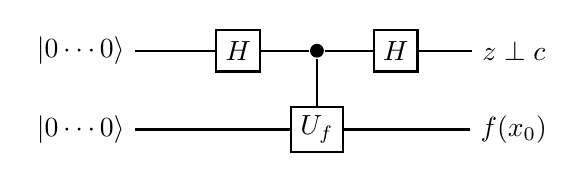
\begin{tikzpicture}[thick]
    %
    % `operator' will only be used by Hadamard (H) gates here.
    % `phase' is used for controlled phase gates (dots).
    % `surround' is used for the background box.
    \tikzstyle{operator} = [draw,fill=white,minimum size=1.5em] 
    \tikzstyle{phase} = [fill,shape=circle,minimum size=5pt,inner sep=0pt]
    \tikzstyle{surround} = [fill=blue!10,thick,draw=black,rounded corners=2mm]
    \tikzstyle{symbol} = [minimum size=5pt,inner sep=0pt]
    
    \node at (0,0) (begin1) {$\ket{0\cdots 0}$};
    \node[operator] (op1) at (2,0) {$H$} edge [-] (begin1);
    \node[phase] (p1) at (3,0) {} edge [-] (op1);
    \node[operator] (op2) at (4,0) {$H$} edge [-] (p1);
    \node at (5.5,0) (end1) {$z\perp c$} edge [-] (op2);
    
    \node at (0,-1) (begin2) {$\ket{0\cdots 0}$};
    \node[operator](U) at (3,-1) {$U_f$} edge [-] (begin2);
    \node at (5.5,-1) (end2) {$f(x_0)$} edge [-] (U);
    \draw[-] (p1) -- (U);
    
\end{tikzpicture}
\end{center}



Finally, from linear algebra over the field $Z_2$ (meaning 0 and 1 are the only allowed scalars, and vector addition is performed using $\oplus$),  if we have an $n$ dimensional
vector space of $Z_2$, and we have  $n-1$ linearly independent vectors, then we may compute a vector $c$ that is orthogonal to each of these vectors. Moreover, it can 
be shown that if we 
evaluate the above circuit $cn$ times, where $c$ is a sufficiently large constant, then we will observe $n-1$ linearly independent vectors with a probability that converges
to one exponentially fast.  \qed

\section*{Quantum Fourier Transform}

The \textbf{quantum Fourier transform (QFT)} on $n$-qubit vectors is a unitary transformation, denoted $F_n$,  for which, given basis state vector $\ket{y}$
\[F_n\ket{y} = 2^{-n/2}\sum_{x} e^{\frac{2\pi ixy}{2^n}}\ket{x},\]
where $xy$ denotes the product of $x$ with $y$, where $0\leq x,y\leq 2^{n}-1$.
We may express $F_n$ has a $2^n\times 2^n$ matrix, where column $y$ of the matrix is $F_n\ket{y}$, $y=0,\ldots,2^{n}-1$, and row $x$ of column $y$ equals
$e^{\frac{2\pi ixy}{2^n}}/2^{n/2}$.


\textbf{Example 19.} Provide the $F_1$ and $F_2$ matrices.


\newpage
The \textbf{inverse quantum Fourier transform (IQFT)}, on $n$-qubit vectors, denoted $F_n^{-1}$, is defined similarly as
\[F_n^{-1}\ket{y} = 2^{-n/2}\sum_{x} e^{\frac{-2\pi ixy}{2^n}}\ket{x},\]

\textbf{Example 20.} Provide the $F_1^{-1}$ and $F_2^{-1}$ matrices.

\newpage
\subsection*{Optimal phase estimation}

In this section we provide an interesting application of QFT called \textbf{optimal phase estimation}, which is the problem of estimating the eigenvalue of a
unitary transformation $U$. The term \textit{phase} comes from the fact that every complex number $c$ can be written in the form $re^{\phi i}$, where $r$ is called the \textbf{modulus}
and $\phi$ the \textbf{phase (angle)}. Now, since $U$ is unitary, it can be shown that each of it's eigenvalues has a modulus equal to 1, in which case estimating its eigenvalue
reduces to estimating its phase. 

In what follows we assume that the phase to be estimated has the form $\phi = 2\pi(x/2^n + \delta)$, where $x=x_{n-1}\cdots x_1x_0$ is an $n$-bit integer, and $|\delta| <= 1/2^{n+1}$.
In other words, we think of $\phi$ as being some fraction $f$ of $2\pi$, where $0\leq f < 1$, where the best $n$-bit approximation of $f$ is $x/2^n$. Viewing it this way, 
$\delta$ then becomes the error when approximating $f$ as $x/2^n$. 

To simplify matters, let's first assume that $\delta=0$, meaning that $f=x/2^n$. Moreover, assume we have access to an eigenvector $\ket{u}$ of $U$ whose eigenvalue has phase 
$\phi$. Notice how a circuit that consists of a $U$ gate, and has input $\ket{u}$, gives an output that cannot tell us much about $\phi$, but can only give us information about the 
relative moduli of the components $u_1$ and $u_2$ of $\ket{u}$. Thus a more subtle approach is needed. To this end, in addition to $\ket{u}$, we assume access to 
control-$U^{2^j}$ gates, where $j=0,1,\ldots,n-1$. These gates allow us to contruct a circuit, called the \textbf{phase-estimation circuit} whose upper input is the $n$-dimensional signed-basis vector $\ket{+\cdots +}$ 
that serves as the ``control vector'' that controls the control-$U^{2^j}$ gates,
and whose lower input is $\ket{u}$, which is sequentially passed through as target for each of the $n$ control gates. A picture of this circuit is shown below for the case $n=3$.


\begin{center}
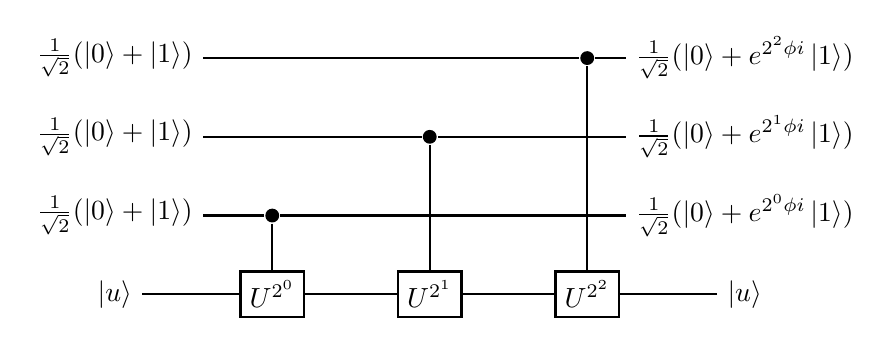
\begin{tikzpicture}[thick]
    %
    % `operator' will only be used by Hadamard (H) gates here.
    % `phase' is used for controlled phase gates (dots).
    % `surround' is used for the background box.
    \tikzstyle{operator} = [draw,fill=white,minimum size=1.5em] 
    \tikzstyle{phase} = [fill,shape=circle,minimum size=5pt,inner sep=0pt]
    \tikzstyle{surround} = [fill=blue!10,thick,draw=black,rounded corners=2mm]
    \tikzstyle{symbol} = [minimum size=8pt,inner sep=0pt]
    
    \node at (0,0) (begin1) {$\frac{1}{\sqrt{2}}(\ket{0}+\ket{1})$};
    \node[phase] (p1) at (6,0) {} edge [-] (begin1);
    \node at (8,0) (end1) {$\frac{1}{\sqrt{2}}(\ket{0}+e^{2^2\phi i}\ket{1})$} edge [-] (p1);
    
    \node at (0,-1) (begin2) {$\frac{1}{\sqrt{2}}(\ket{0}+\ket{1})$};
    \node[phase] (p2) at (4,-1) {} edge [-] (begin2);
    \node at (8,-1) (end2) {$\frac{1}{\sqrt{2}}(\ket{0}+e^{2^1\phi i}\ket{1})$} edge [-] (p2);
    
    \node at (0,-2) (begin3) {$\frac{1}{\sqrt{2}}(\ket{0}+\ket{1})$};
    \node[phase] (p3) at (2,-2) {} edge [-] (begin3);
    \node at (8,-2) (end3) {$\frac{1}{\sqrt{2}}(\ket{0}+e^{2^0\phi i}\ket{1})$} edge [-] (p3);
    
    \node at (0,-3) (begin4) {$\ket{u}$};
    \node[operator] (op3) at (2,-3) {$U^{2^0}$} edge [-] (begin4);
    \node[operator] (op2) at (4,-3) {$U^{2^1}$} edge [-] (op3);
    \node[operator] (op1) at (6,-3) {$U^{2^2}$} edge [-] (op2);
    \node at (8,-3) (end4) {$\ket{u}$} edge [-] (op1);
    
    \draw[-] (p1) -- (op1);
    \draw[-] (p2) -- (op2);
    \draw[-] (p3) -- (op3);
    
\end{tikzpicture}
\end{center}

At first glance, this circuit may seem confusing, since it shows that target vector $\ket{u}$ leaves the circuit apparently unchanged,
 while the control inputs \textit{have} changed. How can this be? Isn't it the other way around: the control inputs don't change, while the target may change depending on 
 the control values? To answer this, we leave it as an exercise to prove the following fact about control-$U$ gate. If the input is $\ket{0}\otimes \ket{u}$, where $\ket{0}$ is
 the control bit, then the output is $\ket{0}\otimes \ket{u}$. On the other hand, if the input is $\ket{1}\otimes \ket{u}$, then the output can be writen 
 as $\ket{1}\otimes U\ket{u}$. Furthermore, given this fact, if $\ket{u}$ is an eigenvector of $U$ with corresponding eigenvalue $e^{\phi i}$, then an input of 
 $\ket{1}\otimes U\ket{u}$ yields the output  $\ket{1}\otimes e^{\phi i}\ket{u} = e^{\phi i}\ket{1}\otimes \ket{u}$. This follows from the tensor product identity
 \[c(\ket{u})\otimes \ket{v} = (c\ket{u})\otimes \ket{v} = \ket{u}\otimes (c\ket{v})\]
 for any complex scalar $c$. Finally, this result can be generalized for the generalization of the circuit shown above, where there are $n$  control qubits. Indeed, 
 if $\ket{y}$ is the 
 is an $n$-qubit basis state vector that serves as control, then the output of the circuit will be $c\ket{y}\otimes \ket{u}$, where $c = e^{\frac{2\pi ixy}{2^n}}$.
 
\textbf{Example 21.} Verify that, if the control vector is $\ket{y}=\ket{110}$, then the circuit output is $e^{\frac{3\pi ix}{2}}\ket{110}\otimes \ket{u}$.
 



\newpage
It is left as an exercise to show that, for each of the other seven basis-state control inputs $\ket{y}$, the circuit output will equal
$e^{\frac{\pi ixy}{4}}\ket{y}\otimes \ket{u}$.

From the above discussion, and by linearity over the $2^n$ different basis-state control vectors, it follows that the phase-estimation circuit output is 
thus 
\[(\frac{1}{2^{n/2}}\sum_{y}e^{\frac{2\pi ixy}{2^n}}\ket{y})\otimes \ket{u}.\]
In other words, the target bits remain constant, while the control bits yield $F_n\ket{x}$, the Fourier transform of $\ket{x}$! Thus, to measure $\ket{x}$ it is sufficient 
to apply $F_n^{-1}$ to the upper $n$ output qubits. Therefore, in the case that $\phi = 2\pi x/2^n$ for some $n$-bit nonnegative integer $n$, the phase angle $\phi$ can be 
exactly computed. 

Now assume that $\phi = 2\pi( x/2^n + \delta)$, where $|\delta| \leq 1/2^{n+1}$. In this case, after applying $F_n^{-1}$ to the upper $n$ qubits of the phase estimation circuit,
there is no guarantee that the output will measure as $\ket{x}$. However, we can compute a lower bound on the probability that $\ket{x}$ is measured. First notice that 
the output of the upper $n$ qubits of the phase estimation circuit is now
\[\frac{1}{2^{n/2}}\sum_{y}e^{\frac{2\pi ixy}{2^n} + 2\pi iy\delta}\ket{y} = \frac{1}{2^{n/2}}\sum_{y}e^{\frac{2\pi ixy}{2^n}}e^{2\pi iy\delta}\ket{y}.\]
Applying $F_n^{-1}$ to this vector, and using applying linearity, yields
\[F_n^{-1}(\frac{1}{2^{n/2}}\sum_{y}e^{\frac{2\pi ixy}{2^n}}e^{2\pi iy\delta}\ket{y}) = \]
\[\frac{1}{2^{n/2}}\sum_{y}e^{\frac{2\pi ixy}{2^n}}e^{2\pi iy\delta}F_n^{-1}(\ket{y}) = \]
\[\frac{1}{2^{n/2}}\sum_{y}e^{\frac{2\pi ixy}{2^n}}e^{2\pi iy\delta}(\frac{1}{2^{n/2}}\sum_ze^{\frac{-2\pi izy}{2^n}}\ket{z}) = \]
\[\frac{1}{2^n}\sum_y\sum_z e^{\frac{2\pi ixy}{2^n}}e^{2\pi iy\delta}e^{\frac{-2\pi izy}{2^n}}\ket{z} = \]
\[\frac{1}{2^n}\sum_z(\sum_y e^{\frac{2\pi i(x-z)y}{2^n}}e^{2\pi iy\delta})\ket{z},\]
where in this final expression we see that the $\ket{z}$ component is equal to 
\[\frac{1}{2^n}\sum_y e^{\frac{2\pi i(x-z)y}{2^n}}e^{2\pi iy\delta}.\]
Moreover, the component we are interested in is $\ket{z} = \ket{x}$, since this is the one we hope to measure. In this case the component equals
\[\frac{1}{2^n}\sum_ye^{2\pi iy\delta} = \frac{1}{2^n}\sum_{y=0}^{2^n - 1} (e^{2\pi i\delta})^y).\]
Furthermore, applying the geometric series formula
\[\sum_{y=0}^k a^y = \frac{1-a^{k+1}}{1-a},\]
we get 
\[\frac{1}{2^n}\sum_{y=0}^{2^n - 1} (e^{2\pi i})^y) = \frac{1}{2^n}\frac{1-e^{2\pi i\delta 2^n}}{1-e^{2\pi i\delta}}.\]
Hence, in order to obtain a lower bound on the likelihood of measuring $\ket{x}$, we must get a lower bound on the square of the modulus of 
\[\frac{1}{2^n}\frac{1-e^{2\pi i\delta 2^n}}{1-e^{2\pi i\delta}}.\]

To begin, first notice that, since $|\delta|\leq \frac{1}{2^{n+1}}$, we have $2^n|\delta| \leq \frac{1}{2}$. Moreover, the following mathematical facts, whose proof is left
as an exercise,  are needed.
\begin{enumerate}

\item  $2z \leq \sin\pi z \leq \pi z$, for all $z\in[0,1/2]$

\item $|1-e^{\phi i}| = 2|\sin\frac{\phi}{2}|$
\end{enumerate}

Using the above facts, we have that the probability of measuring $\ket{x}$ after applying $F_n^{-1}$ to the upper $n$ qubits of the output of the phase estimation circuit,
is equal to 
\[\left|\frac{1}{2^{n}}\frac{(1-e^{2\pi i\delta 2^n})}{(1-e^{2\pi i\delta})}\right|^2 = \frac{1}{2^{2n}}\frac{ 4\sin^2(\pi\delta 2^n)}{4\sin^2(\pi \delta)}\geq \]

\[\frac{1}{2^{2n}}\frac{4\delta^2 2^{2n}}{\pi^2 \delta^2} = \frac{4}{\pi^2}.\]















\newpage
\section*{Shor's Factoring Algorithm}

Given a composite number $N > 1$, consider the problem of finding a \textbf{factor} of $N$; i.e. a number $m$ for which i) $1 < m < N$ and ii) $m$ divides $N$, which is denoted
as $m | N$.
Currently there is no known classical algorithm for finding a factor of $N$ in polynomial time, i.e. time $T(N) = \mbox{O}(\log^k N)$, for some integer $k > 0$ (why do we use
$\log N$ instead of $N$?).
However, in this section we describe a polynomial-time quantum algorithm such that, with probability at least 1/2,  finds a factor of $N$, if one exists. Moreover, by re-running the algorithm,
say $f$ times, then with probability at least $1-1/2^f$ one of the $f$ iterations will find a factor of $N$, and so the algorithm allows us to find a factor of $N$ in polynomial-time
with arbitrarily high probability.

To begin, consider $a\in \{2,\ldots,N-1\}$ for which $\mbox{gcd}(a,N)=1$ (Note:  if $\mbox{gcd}(a,N) > 1$, then Euclid's polynomial-time algorithm may be used to find a factor
that is common to both  $a$ and $N$). Then it is an exercise to show that there is a least positive integer $r < N$, called the \textbf{period} of $a$,
 for which $a^r = 1 \mbox{ mod } N$. 
Moreover, if $r$ is even then we have $N|(a^r-1)$ which implies, by difference of squares,
\[N| (a^{r/2}-1)(a^{r/2}+1).\]
Thus, so long as neither $(a^{r/2}-1)$ nor $(a^{r/2}+1)$ is divisible by $N$, i.e. $a^{r/2} \mbox{ mod } N\not=\pm 1$, then either $a^{r/2}-1$ or $a^{r/2}+1$ shares a common factor with
$N$. The following Theorem is stated without proof (please refer to the article by A. Ekert and R. Jozsa in Reviews of Modern Physics, Volume 68, Issue 3, 1996).

\textbf{Theorem 10.} Suppose $N$ has the prime factorization $N=p_1^{\alpha_1}\cdots p_s^{\alpha_s}$, $a$ is uniformly and randomly selected, and satisfies both $1 < a < N$ and 
$\mbox{gcd}(a,N)=1$.
Then with probability at least $1-1/2^{s-1}$ the period $r$ of $a$ is even, and either 
 $a^{r/2}-1$ or  $a^{r/2}+1$ shares a common factor with $N$.
 
\newpage
\textbf{Example 22.} Verify Theorem 10 for $N=20$. 


\newpage

Thus, according to Theorem 10, with arbitrarily high probability one can  find an $a$ for which either $(a^{r/2}-1)$ or $(a^{r/2}+1)$ shares a common factor with $N$. Unfortunately, once such an
$a$ is found, there is no known efficient classical algorithm for computing $a$'s period $r$, and thus no known efficient way of checking if a correct $a$ has been selected.
Hence, we now focus on the problem of efficiently computing $r$ with a quantum algorithm.

\subsection*{Computing a period using the method of continued fractions}

To begin, suppose that $N$ is an $m$-bit number, integer $n > 2m$ is fixed, and $a\in \{2,\ldots,N-1\}$ has been randomly selected, where $\mbox{gcd}(a,N)=1$. 
Suppose we have access to an oracle
for which, if we give the oracle the values $N$, $a$, and $n$, the oracle returns a positive integer $x$ for which $x/2^n$ is the best $n$-bit approximation of $k/r$,
and is hence within $1/2^n$, where 
$r$ is the period of $a$ relative to $N$, and $k\in\{1,\ldots,r\}$ is randomly selected from $\{1,2,\ldots,r\}$. In what follows we describe how to 
compute $k$ and $r$ given $x$.

First note that, for a given $r$, there can be at most one $k$ for which $k/r$ is within $1/2^n$ of $x/2^n$. For consider $k_1/r$ and $k_2/r$ with $k_1 \not= k_2$. Then 
\[\frac{1}{2^{n-1}} = \frac{1}{2^n} + \frac{1}{2^n} \geq |\frac{k_1}{r} - \frac{x}{2^n}| + |\frac{x}{2^n}-\frac{k_2}{r}| \geq \]
\[|\frac{k_1}{r} - \frac{x}{2^n} + \frac{x}{2^n}-\frac{k_2}{r}| = |k_1-k_2|/r > 1/r > 1/N,\]
which implies that $1/2^{n-1} > 1/N$, i.e. $N > 2^{n-1}$, and that $N$ is at least an $n$-bit number. But this contradicts the assumption that 
$N$ is an $m$-bit number, and $n > 2m$.
Therefore, given $x$, $n$, and $r$, there is a unique fraction $k/r$ for which $x/2^n$ is within $1/2^n$ of $k/r$.

We next look at how to compute $k$ and $r$ by computing the \textit{convergents} of $x/2^n$. This is done by writing $x/2^n$ as a continued fraction.

\newpage
\textbf{Example 23.} The continued fraction of $27/64$ is 
\[\frac{1}{2+\frac{1}{2+\frac{1}{1+\frac{1}{3+\frac{1}{3}}}}},\]
and the convergents are thus 
\[\frac{1}{2}, \mbox{  } \frac{1}{2+\frac{1}{2}} = 2/5, \mbox{  } \frac{1}{2+\frac{1}{2+\frac{1}{1}}} = 3/7,  \mbox{  }\frac{1}{2+\frac{1}{2+\frac{1}{1+\frac{1}{3}}}} = 8/19, 
 \mbox{  } \frac{1}{2+\frac{1}{2+\frac{1}{1+\frac{1}{3+\frac{1}{3}}}}} = 27/64.\]

\newpage
The following theorem is stated without proof (see ``An Introduction to the Theory of Numbers' by G. H. Hardy and E. M. Wright, 
Oxford University Press, Oxford, 1979).

\textbf{Theorem 11.} Given fraction $\theta$, if fraction $p/q$, $\mbox{gcd}(p,q)=1$ satisfies $|\theta - \frac{p}{q}| < \frac{1}{2q^2}$, then $p/q$ is a convergent of $\theta$.

\textbf{Corollary 3.} The fraction $k/r$ is a convergent of $x/2^n$, provided $\mbox{gcd}(k,r)=1$.

\textbf{Proof of Corollary 3.} We have 
\[|x/2^n-k/r| \leq \frac{1}{2^n} < \frac{1}{2(2^m)^2} < \frac{1}{2r^2},\]
and so, by Theorem 10, $k/r$ is a convergent of $x/2^n$. \qed

We leave it as an exercise to show that $x/2^n$ has exactly one convergent $p/q$ for which i) $q \leq r$, and ii) 
$|x/2^n-p/q| < \frac{1}{2r^2}$. 


\textbf{Example 24.} Consider the case where $N=21$, $m=5$, $n=11$, $a=17$, and $r=6$ (verify that $17^6 \mbox{ mod } 21 = 1$). Determine $x$ in case the oracle selects
i) $k=1$, ii) $k=5$. For both cases verify that $k/6$ is a convergent for $x/2^{11}$, and that it is the only convergent that satisfies the inequality of Corollary 3, and 
whose denominator does not exceed $5$ bits. 







\newpage
Note that any fraction $x/2^n$ has a finite number of convergents, and that they may be computed in polynomial time with resepct to $n$, and hence with respect to $m=\log N$.
This is due to the fact that the distance between two convergents decreases exponentially fast (see the Hardy and Wright reference as cited above).

It should also be emphasized that the method of continued fractions may only be used when $\mbox{gcd}(r,k)=1$, i.e. $k$ and $r$ are \textbf{relatively prime}. 
And, since the $k$ that corresponds with the  oracle's returned $x$ value is randomly selected from $\{1,\ldots,r\}$, it  does not guarantee a relatively prime $(k,r)$ pair. However, it can be shown (see the Ekert reference cited above)
that the probability of selecting $k$ for which $\mbox{gcd}(r,k)=1$ is at least $1/\ln r \geq 1/m$. Thus, by making $\mbox{O}(m)$ queries to the oracle, with
arbitrarily high probability one of the returned $x$ values will 
produce a convergent $k/r$ for which $k$ is relatively prime with $r$, in which case the continued-fraction method will yield the correct $k$ and $r$.



So far the presentation has relied solely on basic number theory. However, we now show how to replace the oracle with the phase estimation circuit. We know that applying 
the inverse Fourier transform to the circuit will result in an observation that has a probability of at least $4/\pi^2$ of returning $x$, such that
$x/2^n$ is the best $n$-bit approximation of $f$ where $\phi = 2\pi f$ is the phase of an eigenvalue of some unitary transformation $U$. Thus, in order to use the optimal 
phase estimation circuit, what is needed is a unitary transformation $U$ whose eigenvalues have phases equal to $2\pi k/r$, where $r$ is the order of $a$.

\textbf{Theorem 12.} Given $N$ and $1 < a < N$ for which $\mbox{gcd}(a,N)=1$, the transformation 
 \[U_a\ket{y} = \ket{ay\mbox{ mod } N}\]
 is a unitary transformation with eigenvalue  $e^{2\pi i\frac{k}{r}}$, for all $k=1,\ldots,r$. and corresponding eigenvector 
 \[\ket{u_k} = r^{-1/2}\sum_{j=0}^{r-1}e^{-\frac{2\pi ikj}{r}}\ket{a^j\mbox{ mod } N}.\]

\textbf{Proof of Theorem 12.} First notice that $U_a$ is unitary since the transformation $U_a$ is one-to-one. Indeed, if
$ay_1 \mbox{ mod } N = ay_2 \mbox{ mod } N$, then necessarily $N|a(y_1-y_2)$, and, since $a$ and $N$ are relatively prime, it implies that $N|(y_1-y_2)$. But the only way this
can happen is if $y_1-y_2 =0$ (why ?), and so we must have $y_1=y_2$. 

We leave it as an exercise (see Exercises) to show that $\ket{u_k}$ as defined in the theorem is an eigenvector of $U_a$ with corresponding eigenvalue $e^{2\pi i\frac{k}{r}}$.
\qed


There is only one problem with the unitary transformation described in Theorem 12: the target qubits of the optimal phase estimation circuit must be prepared with an eigenvector, but the eigenvectors of $U_a$ all depend on the unknown
value $r$. However, it is an exercise to show that
\[r^{-1/2}\sum_{k=1}^r\ket{u_k} = \ket{1},\]
and so the target qubits may be prepared with $\ket{1}$ which is a superposition of the $r$ different eigenvectors (one for each possible value of $k$).


\newpage
We now summarize the steps of Shor's algorithm. The algorithm below assumes that $N$ has at least one nontrivial factor, and returns one such factor.
Note: the algorithm uses the \texttt{Continue} statement which has the effect of passing control back to the beginning of the \texttt{while} loop.

\textbf{Shor's Algorithm} for computing $\mbox{\texttt{factor}}(N)$

\begin{itemize}
\renewcommand{\labelitemi}{}
\renewcommand{\labelitemii}{}
\renewcommand{\labelitemiii}{}

\item While a factor has yet to be returned,

\begin{itemize}
\item Randomly select $a\in\{2,\ldots,N-1\}$.
\item $d = \mbox{gcd}(a,N)$.
\item If $d \not= 1$,

\begin{itemize}
\item Return $d$.
\end{itemize}

\item $r = \mbox{find\_period}(a,N)$
\item If $r$ is odd,

\begin{itemize}
\item Continue.
\end{itemize}

\item If $a^{r/2} \mbox{ mod } N = \pm 1$,

\begin{itemize}
\item Continue.
\end{itemize}

\item $d = \mbox{gcd}(a^{r/2}-1,N)$.
\item If $d \not= 1$,

\begin{itemize}
\item Return $d$.
\end{itemize}

\item Return $\mbox{gcd}(a^{r/2}+1,N)$.

\end{itemize}

\end{itemize}

\newpage
The only part of the above algorithm that uses quantum computing is $\mbox{find\_period}(a,N)$, which is summarized below.


\textbf{\texttt{find\_period}(a,N)}.

\begin{itemize}
\renewcommand{\labelitemi}{}
\renewcommand{\labelitemii}{}
\renewcommand{\labelitemiii}{}

\item Let $m = \lfloor\log N\rfloor + 1$.
\item Let $n=2m+1$.
\item While the period $r$ of $a$ has yet to be found,


\begin{itemize}

\item Evaluate the phase optimization circuit using $U=U_a$, and input $\ket{0^n}\ket{1}$.
\item Let $\ket{y}$ denote the circuit's control output.
\item $\ket{x} = F_n^{-1}\ket{y}$.
\item Use the method of continued fractions to determine the convergent $k/r$ of $x/2^n$  for which
it is the unique fraction that satisfies
\[|x/2^n-k/r|  < \frac{1}{2r^2},\]
and for which $r$ can be expressed in at most $m$ bits. 

\item If no such $k/r$ exists, then continue.


\item If $a^r \mbox{ mod } N = 1$,

\begin{itemize}

\item Return $r$.

\end{itemize}


\end{itemize}


\end{itemize}

For the \texttt{while}-loop to terminate (i.e. for the correct period to be found), it must happen that i) $\mbox{gcd}(k,r)=1$ and ii) $x/2^n$ is in fact the best $n$ bit approximation 
of $k/r$. The former happens with probability at least $1/m$, while the latter with probability at leat $4/\pi^2$. Therefore, the expected number of iterations is linear in $m$.


\newpage
\section*{Grover's Algorithm} 

Consider a Boolean function $f:\{0,1\}^{n}\rightarrow \{0,1\}$ for which there is only one $\omega\in\{0,1\}^n$ for which $f(\omega)=1$, and thus $f(\vec{x})=0$ for all 
$\vec{x}\not=\omega$. Moreover, assume that an oracle knows the value of $\omega$, and you know nothing about the structure of $f$, but are able to query the oracle, e.g.
$\mbox{query}(\vec{x})$ is answered with ``no'' iff $\vec{x}\not=\omega$. Thus, learning the value $\omega$ will require an exponential number of queries on average.

Now suppose the oracle provides a quantum circuit for the unitary transformation $U_{\omega}$, where
\[U_{\omega}\ket{x} =\left\{\begin{array}{ll} 
\ket{x} & \mbox{ if } \vec{x}\not=\omega \\
-\ket{x} & \mbox{ if }\vec{x}=\omega \\
\end{array}\right.
\]
Thus, $U_{\omega}$ serves the same purpose as the oracle, but now an answer is in the form of a unitary transformation of some input quantum state. In what follows we leverage
the fact that a ``query'' can now be in the form of a superposition of quantum basis states.

To begin, let $\ket{s}$ denotes $H_n\ket{00\cdots 0}$, the $N=2^n$-dimensional signed basis vector 
\[\frac{1}{\sqrt{N}}\sum_{x=0}^{2^n-1}\ket{x}.\]
Moreover, unitary transformation $U_s$ is defined as
\[2\ket{s}\bra{s} - I_N.\]
One can also show that $U_{\omega} = I_N-2\ket{\omega}\bra{\omega}$. One can view $U_{\omega}$ as  reflection through the hyperplane that is perpendicular to $\ket{\omega}$. 
Similarly, one can show that $U_s$ is a reflection through the hyperplane perpendicular to $\ket{s}$, followed by a reflection through the origin.

Grover's algorithm then consists of computing the sequence of vectors $\ket{x_0},\ket{x_1},\ldots,\ket{x_r}$, where $\ket{x_0} = \ket{s}$, and $\ket{x_{i+1}}=U_sU_{\omega}\ket{x_i}$,
for $i=1,2,\ldots,r-1$. Also, $r$ is chosen large enough so that $|\braket{\omega|x_r}|^2$ is sufficiently close to 1, meaning that with probability close to 1, measuring
$\ket{x_r}$ yields $\omega$.

\newpage
\textbf{Example 25.} Show that 
\[\ket{x_1} = U_sU_{\omega}\ket{s} = \frac{N-4}{N}\ket{s} + \frac{2}{\sqrt{N}}\ket{\omega},\] and that 
\[|\braket{\omega|x_1}|^2 = 9(1-\frac{4}{3N})^2\cdot \frac{1}{N}.\]




\newpage
Notice that $U_sU_{\omega}$ may be viewed as a linear transformation over the space spanned by quantum state vectors $\ket{\omega}$ and $\ket{s}$. 

\textbf{Example 26.} Show that 
\[U_sU_{\omega}(a\ket{\omega}+b\ket{s}) = (a+2b/\sqrt{N})\ket{\omega} + (-2a/\sqrt{N} + b(1-4/N))\ket{s}.\]
Conclude that the transformation matrix of $U_sU_{\omega}$ (relative to the space spanned by $\ket{\omega}$ and $\ket{s}$) is equal to
\[A = 
\left(\begin{array}{cc}
1 & 2/\sqrt{N}\\
-2/\sqrt{N} & 1-4/N\\
\end{array}\right).\]


\newpage
In what follows we let $t = \sin^{-1}(1/\sqrt{N})$. 
We leave the derivations of the following facts as exercises.

\begin{enumerate}
\item $A$ has eigenvalues $e^{2ti}$ and $e^{-2ti}$.
\item We have
\[A = M
\left(\begin{array}{cc}
e^{2ti} & 0\\
0 & e^{-2ti}\\
\end{array}\right)
M^{-1},\]
where 
\[M=\left(\begin{array}{cc}
-i & i\\
e^{ti} & e^{-ti}\\
\end{array}\right).\]

\item We have
\[A^r = M
\left(\begin{array}{cc}
e^{2rti} & 0\\
0 & e^{-2rti}\\
\end{array}\right)
M^{-1}\]
\item For $r=\pi/4t = \pi/4\mbox{arcsin}(1/\sqrt{N})\approx \pi\sqrt{N}/4$, we have
\[\left(\begin{array}{cc}
\ket{\omega} & \ket{s}\\
\end{array}\right)
(U_sU_{\omega})^r
\left(\begin{array}{c}
0\\
1\\
\end{array}\right) \approx
\left(\begin{array}{cc}
\ket{\omega} & \ket{s}\\
\end{array}\right)
M
\left(\begin{array}{cc}
i & 0\\
0 & -i\\
\end{array}\right)
M^{-1}
\left(\begin{array}{c}
0\\
1\\
\end{array}\right) = \sec{t}\ket{\omega} -\tan{t}\ket{s},\]
and measuring this quantum-state vector will yield $\ket{\omega}$ with probability at least 
$1-\mbox{O}(1/N)$.


\end{enumerate}


\newpage
\section*{Acknowledgments}

Special thanks to Nelson Minaya, Bernardo Cobos, and other students who have helped identify errors in previous versions of these notes.



\section*{Exercises}

\begin{enumerate}
\renewcommand{\labelenumii}{\alph{enumii}.}

\item Write the basis state vectors corresponding to 

\begin{enumerate}
\item $\ket{11}$.
\item $\ket{2}$.
\item $\ket{010}$.
\item $\ket{6}$.
\end{enumerate}

\item Write the following basis state vectors using ket notation. Note: to save space, all are assumed column vectors, but are written as rows.

\begin{enumerate}
\item $(0,1,0,0)$
\item $(0,0,0,1)$
\item $(0,0,0,0,0,1,0,0)$
\item $(0,0,1,0,0,0,0,0)$
\end{enumerate}

\item For each $i\in \{0,1,2,3\}$, provide a matrix $A_i$ so that, forall $x\in \{0,1,2,3\}$, $A_i \ket{x} = \ket{(x+i)\mbox{ mod } 4}$.

\item Given 
\[
u=\left(\begin{array}{c}
1+i \\
-2+i \\
\end{array}\right)
\mbox{ , }
v=\left(\begin{array}{c}
2i \\
2-i \\
\end{array}\right)
\mbox{ and }
w=\left(\begin{array}{c}
3 \\
-2 \\
\end{array}\right)
\]
compute

\begin{enumerate}
\item $\braket{u|v}$
\item $\braket{v|u}$
\item $\braket{u|u}$
\item $\braket{u|(2+i)v}$
\item $\braket{u+v|w}$
\end{enumerate}


\item Prove the linearity property of the inner product. 

\item Prove the following properties of the inner product.

\begin{enumerate}
\item $\operatorname{Re}(\langle u|v\rangle)\leq |\langle u|v \rangle|$.
\item $\langle u|v\rangle + \langle v|u\rangle = 2\operatorname{Re}(\langle u|v\rangle)$
\item $\langle ku|v\rangle = k^* \langle u|v\rangle$
\item $\langle u+v|w\rangle = \langle u|w\rangle + \langle v|w\rangle$
\end{enumerate}


\item Use the Cauchy-Schwarz inequality to prove the \textbf{triangle inequality}
\[|u|-|v| \leq |u+v|\leq |u| + |v|.\]
Hint: square each side and use the inner-product axioms as well as the results from the previous exercise.

\item Let $a=a_1+a_2i$ and $b=b_1+b_2i$ be two arbitrary complex numbers. By defining $\langle a|b\rangle=a^*b$, verify that all the inner-product axioms are satisfied.

\item Suppose two paths of a photon intersect at a given location. If complex numbers $a$ and $b$ are the amplitudes
of the two paths, then the probability of finding the photon at this location is $P=|a+b|^2$. Show that $P$ satisfies the inequality 
\[(|a|-|b|)^2 \leq P \leq (|a|+|b|)^2.\]
Hint: use the previous two exercises.

\item 
Referring to the previous exercise,
show that, when multiplying $b$ by a random angle $e^{\theta i}$, where $\theta\in [0,2\pi]$ is chosen uniformly at random, then the average probability 
is 
\[E[P(\theta)]=\frac{1}{2\pi}\int_0^{2\pi} P(\theta)d\theta =|a|^2 + |b|^2,\]
where the first equality does not need proof, but rather is the mathematical definition for computing $E[P(\theta)]$.
 Note that this average is the same that one gets  when assuming that the two paths are independent. Hint: find a formula for $P(\theta)$ by computing
 $|a+kb|^2$ using properties of the inner product,
where $k=e^{i\theta}$. Then integrate $P(\theta)$ as indicated above.

\item Use the proof of the Cauchy-Schwarz Theorem, along with properties of the inner product, to prove that if two quantum state vectors $\ket{u}$ and 
$\ket{v}$  satisfy  $\langle u| v\rangle=1$, then necessarily $\ket{u}=\ket{v}$.

\item Verify that  $e_{1}=(1/\sqrt{10},-3\/\sqrt{10})$, $e_{2}=(3/\sqrt{10},1/\sqrt{10})$ is an orthonormal basis. 
Determine coefficients $c_1$ and $c_2$ for which $v=(-1,4)=c_1e_1 + c_2e_2$ 


\item Verify that $e_{1}=(1/\sqrt{3},1/\sqrt{3},1/\sqrt{3})$,  $e_{2}=(-1/\sqrt{2},1/\sqrt{2},0)$,  $e_{3}=(1/\sqrt{6},1/\sqrt{6},-2/\sqrt{6})$ 
is an orthonormal basis. 
Determine coefficients $c_1$, $c_2$, and $c_3$ for which $v=(0.5,-2,3)=c_1e_1 + c_2e_2 + c_3e_3$.

\item Verify that $e_{1}=(1,0,0)$,  $e_{2}=(0,7/\sqrt{53},-2/\sqrt{53})$,  $e_{3}=(0,30/\sqrt{11925},105/\sqrt{11925})$ 
is an orthonormal basis. 
Determine coefficients $c_1$, $c_2$, and $c_3$ for which $v=(0.5,-2,3)=c_1e_1 + c_2e_2 + c_3e_3$.

\item Provide the change-of-basis matrix from $\mathcal{B}_1=\{(1/\sqrt{10},-3\/\sqrt{10}),(3/\sqrt{10},1/\sqrt{10})\}$ to\\
 $\mathcal{B}_2=\{(\frac{1}{\sqrt{5}},\frac{2}{\sqrt{5}}),(\frac{2}{\sqrt{5}},\frac{-1}{\sqrt{5}})\}$.

\item Show that if $u=(u_1,\ldots,u_n)$, then the matrix associated with $\ket{u}\bra{u}$ has $(i,j)$-entry $u_iu_j^*$. Use this to verify that
\[(\ket{u}\bra{u})^{\dagger} = \ket{u}\bra{u}.\]

\item If $\mathcal{B}=\{\vec{v}_1,\ldots,\vec{v}_n\}$ is an orthonormal basis, then provide a formula  the
 matrix representation of the linear transformation
$\ket{v_j}\bra{v_k}$. In particular give a formula for the row-$a$ column-$b$ entry of the matrix.
Hint: Let $\ket{v_j}=(v_{j1},\ldots,v_{jn}$ and  $\ket{v_k}=(v_{k1},\ldots,v_{kn})$.

\item Given $v=(-1,2,6,0)$, determine the projection of $\ket{v}$, onto the subspace having orthonormal basis $u_{1}=\frac{1}{\sqrt{6}}(-1,0,1,2)$ and $u_{2}=\frac{1}{\sqrt{6}}(0,1,-2,1)$.

\item Find the eigenvalues and an orthonormal set of eigenvectors for 
\[
Y=\left(\begin{array}{cc}
0 & -i\\
i & 0\\
\end{array}\right)\mbox{ and }
Z = \left(\begin{array}{cc}
1 & 0 \\
0 & -1 \\
\end{array}\right).\]

\item Prove that, for any two square matrices $A$ and $B$, $(AB)^{\dagger} = B^{\dagger}A^{\dagger}$, and $(A^{\dagger})^{\dagger} = A$.

\item Prove that a normal matrix is Hermitian if and only if it has real eigenvalues.

\item Prove that two eigenvectors of a Hermitian matrix from different eigenspaces must be orthogonal.

\item Matrix $A$ is said to be \textbf{positive} iff $\braket{v|Av}\geq 0$ for all complex $\ket{v}\not=0$. Prove that a positive matrix must be Hermitian.
Hint: use the fact that an arbitrary matrix $A$ can be written as $A=B+iC$, where  $B$ and $C$ are Hermitian. Then show that $C=0$.






%place holder




\item Suppose $U$ is an $n\times n$ unitary matrix whose entries are all ones and zeros. Prove that every row and every column of $U$ has one 1-entry and $n-1$ 0-entries.

\item Given binary word $w=w_1w_2\cdots w_n$ use mathematical induction prove that
\[\ket{w}=\ket{w_1}\otimes \ket{w_2}\otimes \cdots \otimes \ket{w_n}.\]
In words, every  quantum basis-state vector is separable.

\item Let $H$ be the Hadamard matrix, while $X$ is the matrix from Example  6. Compute the following: $H\otimes H$, $X\otimes X$, $H\otimes X$, and $X\otimes H$.

\item Let $I$ be the $n\times n$ identify matrix, while $A$ is an $n\times n$ matrix. Describe in a few sentences the structure of the
 matrices $I\otimes A$ and $A\otimes I$.




\item Show that $\frac{1}{\sqrt{2}}(\ket{00} + \ket{11})$ is an entangled state vector. 




\item 
\label{ex:uniform}
Show that for any $n$-qubit basis state $\ket{y}$
\[H_n\ket{y} = 2^{-n/2}\sum_{x}(-1)^{y\cdot x}\ket{x},\]
where $y\cdot x$ in the exponent means the dot product between $x$ and $y$ (thinking of each as $n$-bit binary vectors), 
and the right summation is over all $n$-qubit basis state vectors.
Hint: Corollary 1 and the fact that $\ket{y}$ may be written as the tensor product of $n$ qubits.


\item Suppose the control input to a c-not gate is $\alpha\ket{0}+\beta\ket{1}$, where $\alpha,\beta\not=0$, while the target input is $\ket{0}$. Prove that the output
vector is non-separable. Is the same true if the roles of the two inputs are reversed? Explain.

\item Prove the following circuit identity. Hint: use matrices.

\begin{center}
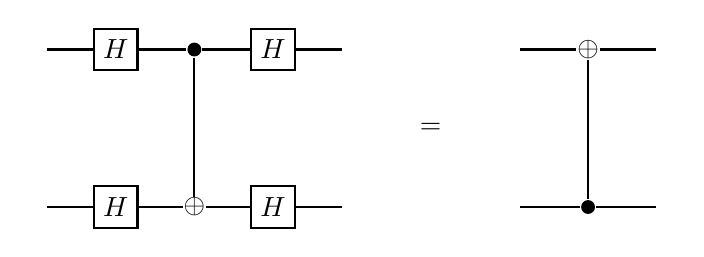
\begin{tikzpicture}[thick]
    %
    % `operator' will only be used by Hadamard (H) gates here.
    % `phase' is used for controlled phase gates (dots).
    % `surround' is used for the background box.
    \tikzstyle{operator} = [draw,fill=white,minimum size=1.5em] 
    \tikzstyle{phase} = [fill,shape=circle,minimum size=5pt,inner sep=0pt]
    \tikzstyle{surround} = [fill=blue!10,thick,draw=black,rounded corners=2mm]
    \tikzstyle{symbol} = [minimum size=5pt,inner sep=0pt]
    
    \node at (0,0) (begin1) {};
    \node[operator] (op1) at (1,0) {$H$} edge [-] (begin1);
    \node[phase] (p1) at (2,0) {} edge [-] (op1);
    \node[operator] (op2) at (3,0) {$H$} edge [-] (p1);
    \node at (4,0) (end1) {} edge [-] (op2);
    
     \node at (5,-1)  {$=$};
    
    \node at (0,-2) (begin2) {};
    \node[operator] (op3) at (1,-2) {$H$} edge [-] (begin2);
    \node[symbol](s1) at (2,-2) {$\oplus$} edge [-] (op3);
    \node[operator] (op4) at (3,-2) {$H$} edge [-] (s1);
    \node at (4,-2) (end2) {} edge [-] (op4);
    \draw[-] (p1) -- (s1);
    
    \node at (6,0) (begin3) {};
   	\node[symbol](s2) at (7,0) {$\oplus$} edge [-] (begin3);
    \node at (8,0) (end3) {} edge [-] (s2);
    
    \node at (6,-2) (begin4) {};
    \node[phase] (p2) at (7,-2) {} edge [-] (begin4);
    \node at (8,-2) (end4) {} edge [-] (p2);
    \draw[-] (p2) -- (s2);
\end{tikzpicture}
\end{center}

\item Prove the correctness of the following circuit. Hint: use matrices.

\begin{center}
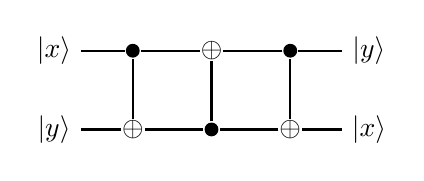
\begin{tikzpicture}[thick]
    %
    % `operator' will only be used by Hadamard (H) gates here.
    % `phase' is used for controlled phase gates (dots).
    % `surround' is used for the background box.
    \tikzstyle{operator} = [draw,fill=white,minimum size=1.5em] 
    \tikzstyle{phase} = [fill,shape=circle,minimum size=5pt,inner sep=0pt]
    \tikzstyle{surround} = [fill=blue!10,thick,draw=black,rounded corners=2mm]
    \tikzstyle{symbol} = [minimum size=5pt,inner sep=0pt]
    
    \node at (0,0) (begin1) {$\ket{x}$};
    \node[phase] (p1) at (1,0) {} edge [-] (begin1);
    \node[symbol](s1) at (2,0) {$\oplus$} edge [-] (p1);
    \node[phase] (p2) at (3,0) {} edge [-] (s1);
    \node at (4,0) (end1) {$\ket{y}$} edge [-] (p2);

    \node at (0,-1) (begin2) {$\ket{y}$};
    \node[symbol](s2) at (1,-1) {$\oplus$} edge [-] (begin2);
    \node[phase] (p3) at (2,-1) {} edge [-] (s2);
    \node[symbol](s3) at (3,-1) {$\oplus$} edge [-] (p3);
    \node at (4,-1) (end2) {$\ket{x}$} edge [-] (s3);
    \draw[-] (p1) -- (s2);
    \draw[-] (p2) -- (s3);
    \draw[-] (p3) -- (s1);
    
\end{tikzpicture}
\end{center}


\item Use the single-qubit adder to create a two-qubit ripple-carry adder.

\item Show that 
\[U_{00} = I, U_{01} = 
\left(\begin{array}{c|c}
I & \\
\hline
 &  X \\
\end{array}\right), \mbox{ and }
 U_{11} = 
\left(\begin{array}{c|c}
X & \\
\hline
 &  X \\
\end{array}\right).
\]

\item 
\label{ex:unitary}
Show that a matrix $A$ whose columns form a permutation of the basis state vectors is unitary.
Hint: describe how to obtain entry $(i,j)$ of $A^t A$.

\item Show that if $U$ is an $n\times n$ unitary matrix, then $U\otimes U$ is an $n^2\times n^2$ unitary matrix.
Hint: use Theorem 5 and the fact that $(A\otimes B)^{\dagger} = A^{\dagger}\otimes B^{\dagger}$ (why ?).

\item Provide the signatures of the eight three-qubit signed basis vectors.

\item Show that $v_{1}=(2/3,-2/3,1/3)$, $v_{2}=(2/3,1/3,-2/3)$, and $v_{3}=(1/3,2/3,2/3)$ an orthonormal set of basis vectors for $\mathcal{R}^3$.
Write the following vectors as linear combinations of these vectors.
\begin{enumerate}
\item $(1,0,0)$
\item $(-1,1,-2)$
\item $(-3,5,1)$
\end{enumerate}


\item Explain why $v_{1}=(1,0,0)$, $v_{2}=(0,1/\sqrt{2},1/\sqrt{2})$, and $v_{3}=(0,0,1)$ is not an orthonormal set of vectors?
 
\item For $n$-bit binary vectors $a,b,c$, show that 
\[a\cdot (b\oplus c)= a\cdot b \oplus a\cdot c,\]
where all dot products are taken modulo 2. Hint: make a truth table or perform a case-by-case analysis for showing the two sides of tne equation must be equal.

\item Use Euclid's algorithm to compute $\mbox{gcd}(a,b)$ for the following values of $a$ and $b$.
\begin{enumerate}
\item $a=36$, $b=111$
\item $a=52$, $b=127$
\item $a=26$, $b=82$
\end{enumerate}

\item For $N=18$ find all values between 2 and 17 that are relatively prime with respect to 18. For each such value, determine its period modulo 18.

\item Prove that if $a\in\{2,\ldots,N-1\}$ satisfies $\mbox{gcd}(a,N)=1$, then there does not exist an $r\in\{1,\ldots,N-1\}$ for which $a^r=0\mbox{ mod }N$

\item Prove that if $a\in\{2,\ldots,N-1\}$ satisfies $\mbox{gcd}(a,N)=1$, then there is a least positive $r\in\{1,\ldots,N-1\}$ for which $a^r=1\mbox{ mod }N$.
Hint: use a counting argument to show that, if the result were not true, then there must exist $r_1,r_2\in\{1,\ldots,N-1\}$ for which
$a^{r_1}=a^{r_2}\mbox{ mod }N$.

\item Verify Thoerem 9 for $N=18$.

\item Find the convergents for each of the following fractions.
\begin{enumerate}
\item $18/25$
\item $31/73$
\item $15/38$
\end{enumerate}

\item Compute $F_3$ and $F_3^{-1}$.

\item Show that, for a positive $N > 2$ and positive $a\in\{2,\ldots,N-1\}$ that is relatively prime with respect to $N$, the mapping
 \[U_a\ket{y} = \ket{ay\mbox{ mod } N}\]
 is a unitary transformation with eigenvalues  $e^{2\pi i\frac{k}{r}}$ 
 and corresponding eigenvectors
 \[\ket{u_k} = r^{-1/2}\sum_{j=0}^{r-1}e^{-\frac{2\pi ikj}{r}}\ket{a^j\mbox{ mod } N},\]
 for all $k=1,\ldots,n$.
 
\item 
\label{exercise:sum}
For positive integer $n$ and for integer $j$ not divisible by $n$, prove that
\[\overset{n-1}{\underset{k=0}{\sum}}e^{\frac{2\pi ijk}{n}}=0.\]
Hint: use the geometric series formula
\[\overset{n-1}{\underset{k=0}{\sum}}a^{k}=\frac{a^{n}-1}{a-1},\]
which is valid when $a$ is a complex number.
 
 \item Show that \[r^{-1/2}\sum_{k=1}^r\ket{u_k} = \ket{1},\]
  

\item  Prove that $2z \leq \sin\pi z \leq \pi z$, for all $z\in[0,1/2]$. Hint: e.g. use calculus with the function $f(z) = \sin\pi z - 2z$ and show that $f(z)$ is an increasing 
function over the interval $[0,1/2]$.

\item Prove that $|1-e^{\phi i}| = 2|\sin\frac{\phi}{2}|$.

\item Suppose that $k/r$ is a convergent of $x/2^n$, and satisfies $|x/2^n-p/q| < \frac{1}{2r^2}$. The prove that there is exactly one convergent $p/q$ (namely $k/r$) for which
 i) $q \leq r$, and ii) 
$|x/2^n-p/q| < \frac{1}{2r^2}$. 
 






    

\end{enumerate}




\newpage
\section*{Exercise Solutions}

\begin{enumerate}
\renewcommand{\labelenumii}{\alph{enumii}.}

\item Note: to save space all basis state vectors are written as row vectors.

\begin{enumerate}
\item $\ket{11} = \ket{3} = (0,0,0,1)$.
\item $\ket{2} = \ket{10} = (0,0,1,0)$.
\item $\ket{010} = (0, 0, 1, 0, 0, 0, 0, 0)$.
\item $\ket{6}=\ket{110} = (0,0,0,0,0,0,1,0)$.
\end{enumerate}

\item We have the following.

\begin{enumerate}
\item $(0,1,0,0)=\ket{01}$
\item $(0,0,0,1) = \ket{3} = \ket{11}$
\item $(0,0,0,0,0,1,0,0)=\ket{5}=\ket{101}$
\item $(0,0,1,0,0,0,0,0)=\ket{010}$
\end{enumerate}




\item We have $A_0=I_4$,
\[
A_1=\left(\begin{array}{cccc}
0 & 0 & 0 & 1 \\
1 & 0 & 0 & 0 \\
0 & 1 & 0 & 0 \\
0 & 0 & 1 & 0 \\
\end{array}\right)
\mbox{ , }
A_2=\left(\begin{array}{cccc}
0 & 0 & 1 & 0 \\
0 & 0 & 0 & 1 \\
1 & 0 & 0 & 0 \\
0 & 1 & 0 & 0 \\
\end{array}\right)
\mbox{ and }
A_3=
\left(\begin{array}{cccc}
0 & 1 & 0 & 0 \\
0 & 0 & 1 & 0 \\
0 & 0 & 0 & 1 \\
1 & 0 & 0 & 0 \\
\end{array}\right).
\]





\item We have the following.

\begin{enumerate}
\item $\braket{u|v}=-3+2i$
\item $\braket{v|u}=-3-2i$
\item $\braket{u|u}=7$
\item $\braket{u|(2+i)v}=(2+i)\braket{u|v}=(2+i)(-3+2i)=-8+i$
\item $\braket{u+v|w}=3-9i$
\end{enumerate}


\item We have
\[\braket{u|hv+kw} = \sum_{i=1}^nu_i^*(hv_i + kw_i) =  \sum_{i=1}^n (hu_i^*v_i + ku_i^*w_i) = \]
\[\sum_{i=1}^n hu_i^*v_i  + \sum_{i=1}^n ku_i^*w_i=\]
\[h\sum_{i=1}^n u_i^*v_i  + k\sum_{i=1}^n u_i^*w_i=h\braket{u|v} + k\braket{u|w}.\]




\item We have the following proofs.

\begin{enumerate}
\item In general, for any complex number $a+bi$, we have 
\[\operatorname{Re}(a+bi) = a\leq |a+bi| =\sqrt{a^2+b^2}\] 
iff
$a^2\leq a^2+b^2$, which is true for all real $a$.

\item In general, 
\[(a+bi) + \overline{a+bi} = (a+bi) + (a-bi) = 2a = 2\operatorname{Re}(a+bi).\]


\item By the symmetry property and linearity property (see previous exercise) of the inner product, we have
\[\braket{ku|v} = \braket{v,ku}^* = (k\braket{v|u})^* = k^*\braket{v|u}^* = k^*\braket{u|v}.\]

\item By the symmetry property and linearity property (see previous exercise) of the inner product, we have
\[\braket{u+v|w} = \braket{w|u+v}^* = (\braket{w|u} + \braket{w|v})^* = \braket{w|u}^* + \braket{w|v}^* = \braket{u|w} + \braket{v|w}.\]

\end{enumerate}


\item It suffices to show that 
\[(|u|-|v|)^2 \leq |u+v|^2\leq (|u| + |v|)^2.\]
With this in mind,
\[|u+v|^2 = \braket{u+v|u+v} = \braket{u|u}+\braket{u|v} + \braket{v|u} + \braket{v|v} =\]
\[|u|^2 + 2\operatorname{Re}(\braket{u|v}) + |v|^2\leq |u|^2 + 2|(\braket{u|v})| + |v|^2 \leq |u|^2 + 2|u||v| + |v|^2 = (|u|+|v|)^2,\]
where the last inequality is due to the Cauchy-Schwarz inequality. The lower-bound inequality is proved similarly.





\item The proofs are identical to the proofs for the $n$-dimensional case, except  now $\overset{n}{\underset{i=1}{\sum}}$ can be dropped from each expression,
since $n=1$. Another way of viewing this is that the inner-product axioms for $n$-dimensional complex vectors are a result of the properties of 
(one-dimensional) complex numbers.



\item By the previous exercise, the inner-product axioms and theorems hold for one-dimensional complex numbers $a$ and $b$. Thus, by the triangle inequality
we have
\[(|a|-|b|)^2 \leq P = |a+b|^2 \leq (|a|+|b|)^2.\]



\item We have 
\[P(\theta)=|a+e^{\theta i}b|^2 = \braket{a+e^{\theta i}b|a+e^{\theta i}b}^2 = 
|a|^2 + |b|^2  + 2\operatorname{Re}(\braket{a|e^{\theta i}b}) =\]\[ |a|^2 + |b|^2 + \alpha_1\cos\theta + \beta_1\sin\theta,\]
for some constants $\alpha_1$ and $\beta_1$ that depend on the real and complex parts of  $a$ and $b$.
However,
\[\frac{\alpha_1}{2\pi}\int_0^{2\pi}\cos\theta d\theta = \frac{\beta_1}{2\pi}\int_0^{2\pi}\sin\theta d\theta = 0,\]
meaning that the last two terms will average to zero. Therefore, the average probability $E[P(\theta)]$ is equal to the sum of the two constant terms, namely
$|a|^2 + |b|^2$.

\item In the proof of the Cauchy-Schwarz Theorem, if  $\langle u|v\rangle=1$, then when setting $t=1$  we get
\[|\ket{u}-\ket{v}|^2 = \langle u-v|u-v\rangle = \langle u|u\rangle - \langle u|v\rangle - [\langle v|u \rangle-\langle v|v\rangle]=\]
\[1-1-(1-1) = 0,\]
which implies $|\ket{u}-\ket{v}|=0$. But by the positivity property of the inner product, this implies that $\ket{u}-\ket{v}=0$, and that $\ket{u}=\ket{v}$.



\item $c_1 = \langle v|e_1\rangle = \frac{-13}{\sqrt{10}}$, $c_2 = \langle v|e_2\rangle = \frac{1}{\sqrt{10}}$



\item $c_1 = \langle v|e_1\rangle = \frac{\sqrt{3}}{2}$, $c_2 = \langle v|e_2\rangle = \frac{-5}{2\sqrt{3}}$, $c_3 = \langle v|e_3\rangle = \frac{-15}{2\sqrt{3}}$

\item $c_1 = \langle v|e_1\rangle = 0.5$, $c_2 = \langle v|e_2\rangle = \frac{-20}{\sqrt{53}}$, $c_3 = \langle v|e_3\rangle = \frac{255}{\sqrt{11925}}$



\item 
Let $a_{ij}$ denote the $(i,j)$-entry of the change-of-basis matrix, $1\leq i,j\leq 2$. Then
\[a_{11} = \langle (\frac{1}{\sqrt{5}},\frac{2}{\sqrt{5}}) | (1/\sqrt{10},-3\/\sqrt{10}) \rangle = -\sqrt{\frac{1}{2}},\]
\[a_{21} = \langle (\frac{2}{\sqrt{5}},\frac{-1}{\sqrt{5}}) | (1/\sqrt{10},-3\/\sqrt{10}) \rangle = \sqrt{\frac{1}{2}},\]
\[a_{12} = \langle (\frac{1}{\sqrt{5}},\frac{2}{\sqrt{5}}) | (3/\sqrt{10},1/\sqrt{10}) \rangle = \sqrt{\frac{1}{2}},\]
and
\[a_{22} = \langle (\frac{2}{\sqrt{5}},\frac{-1}{\sqrt{5}}) | (3/\sqrt{10},1/\sqrt{10}) \rangle = \sqrt{\frac{1}{2}}.\]
Therefore, the matrix is 
\[
\frac{1}{\sqrt{2}}\left(\begin{array}{cc}
-1 & 1\\
1 & 1 \\
\end{array}\right)\]

\item Notice that $\ket{u}\bra{u}$ is the product of an $n\times 1$ matrix with a $1\times n$, and that entry $(i,j)$ of this product is the dot product of
 row $i$ of $\ket{u}$ with column $j$ of $\bra{u}$. But row $i$ of $\ket{u}$ is $u_i$, while column $j$ of $\bra{u}$ is $u_j^*$. Therefore, the product 
 has $(i,j)$-entry $u_iu_j^*$. Finally, by definition, entry $(i,j)$ of $(\ket{u}\bra{u})^{\dagger}$ is the conjugate of entry $(j,i)$ of 
  $(\ket{u}\bra{u})$, namely 
  \[(u_ju_i^*)^* = u_j^*(u_i^*)^*= u_iu_j^*,\]
  which is the $(i,j)$-entry of $\ket{u}\bra{u}$. Therefore, $\ket{u}\bra{u}$ is Hermitian. 




\item Entry $(a,b)$ of the matrix is $v_{ja}v_{kb}^*$.

\item By definition, the projection of $v=(-1,2,6,0)$ onto the subspace having orthonormal basis $u_{1}=\frac{1}{\sqrt{6}}(-1,0,1,2)$ and $u_{2}=\frac{1}{\sqrt{6}}(0,1,-2,1)$
is
\[\ket{u_1}\braket{u_1|v} + \ket{u_2}\braket{u_2|v} = (-7/6,0,7/6,7/3) + (0,-5/3,10/3,-5/3) = (-7/6,-5/3,9/2,2/3).\]


\item For matrix $Y$, eigenvalue $\lambda = 1$ has the one-dimensional eigenspace spanned by 
\[
\frac{1}{\sqrt{2}}\left(\begin{array}{c}
-i\\
1\\
\end{array}\right)\]
while eigenvalue $\lambda = -1$ has the one-dimensional eigenspace spanned by 
\[
\frac{1}{\sqrt{2}}\left(\begin{array}{c}
i\\
1\\
\end{array}\right).\]

For matrix $Z$, eigenvalue $\lambda = 1$ has the one-dimensional eigenspace spanned by 
\[
\left(\begin{array}{c}
1\\
0\\
\end{array}\right)\]
while eigenvalue $\lambda = -1$ has the one-dimensional eigenspace spanned by 
\[
\left(\begin{array}{c}
0\\
1\\
\end{array}\right).\]


\item Suppose $A$ is an $m\times n$ matrix, and $B$ is an $n\times p$ matrix. Then $(AB)^{\dagger}$ is a $p\times m$ matrix whose $(i,j)$-entry is the conjugate
of the $(j,i)$-entry of $AB$ which is equal to 
\[(\sum_{k=1}^n a_{jk}b_{ki})^{*}= \sum_{k=1}^n a_{jk}^*b_{ki}^* = \sum_{k=1}^n (B^{\dagger})_{ik}(A^{\dagger})_{kj}\]
which equals the $(i,j)$-entry of $B^{\dagger}A^{\dagger}$. Finally, since $a_{ji}^*$ is the $(i,j)$-entry of $A^{\dagger}$, the $(i,j)$-entry of $(A^\dagger)^{\dagger}$
is $(a_{ij}^*)^* = a_{ij}$, and so $(A^\dagger)^{\dagger}=A$.

\item  Suppose $A$ is Hermitian. Then by the Spectral Decomposition Theorem, $A$ has at least one eigenvalue $\lambda$, and at least one associated unit eigenvector $\ket{v}$. Then
\[\braket{v|A v} = \braket{v|\lambda v} = \lambda \braket{v|v} = \lambda.\]
Moreover, since $A=A^\dagger$, and, by definition $\braket{v|A v}=\bra{v}^{\dagger}Av$, we have
\[\braket{v|A v} = \bra{v}^{\dagger}A^{\dagger}v = (A\ket{v})^\dagger v = \braket{Av|v} = \braket{\lambda v|v} = \lambda^*.\]
Therefore, $\lambda = \lambda^*$ which implies $\lambda$'s imaginary component is zero; i.e., $\lambda$ is real. 

Conversely, suppose normal matrix $A$ has all real eigenvalues. Then by the Spectral Decomposition Theorem, we may write $A$ as 
\[A = \sum_{v}vP_v,\]
where $v$ is an index variable whose domain is the set of eigenvalues of $A$, and $P_v$ is the projection transformation onto $v$'s eigenspace. 
Therefore, since $v^* = v$ and $P^\dagger = P$, it follows that
\[A^\dagger = (\sum_{v}vP_v)^\dagger = \sum_vv^*P^\dagger = \sum_v vP_v = A.\]

\item Let $\lambda_1\not=\lambda_2$ be two distinct (real) eigenvalues of Hermitian matrix $A$ and suppose $\ket{u}$ and $\ket{v}$ are two eigenvectors for which
$A\ket{u}=\lambda_1\ket{u}$ and $A\ket{v}=\lambda_2\ket{v}$. In what follows, we use the fact (see previous exercise) that, since $A$ is Hermitian, $\braket{Au|v}=\braket{u|Av}$.

Case 1: $\lambda_1 = 0$. Then $\lambda_2\not=0$, and
\[\braket{u|v} = \braket{u|\frac{1}{\lambda_2}Av} = \frac{1}{\lambda_2}\braket{u|Av} = \frac{1}{\lambda_2}\braket{Au|v}= \frac{1}{\lambda_2}\braket{\vec{0}|v} = 0.\]

Case 2: $\lambda_1,\lambda_2 \not= 0$. Then
\[\braket{u|v} = \braket{u|\frac{1}{\lambda_2}Av} = \frac{1}{\lambda_2}\braket{u|Av} = \frac{1}{\lambda_2}\braket{Au|v}= \frac{1}{\lambda_2}\braket{\lambda_1 u|v} =\]
\[\frac{\lambda_1}{\lambda_2}\braket{u|v},\]
which can only be true (since $\lambda_1\not=\lambda_2$) in case $\braket{u|v}=0$.

\item We first show that any $n\times n$ matrix $A$ can be written as $A=B+iC$, where $B$ and $C$ are Hermitian. We define the $B$ and $C$ matrices as follows.
Consider complex entry $a_{rr}=x+yi$ for some $1\leq r\leq n$. Then
we set $b_{rr}=x$ and $c_{rr} = y$. Now suppose $r\not= s$, $a_{rs}=x+yi$, and $a_{sr}=w+zi$. First notice that, if $b_{rs}$ is known to equal $\beta_1 + \beta_2 i$, then, since we 
require $B=B^{\dagger}$, we must have $b_{sr}=b_{rs}^*=\beta_1 - \beta_2 i$. The same holds true for $c_{rs}=\kappa_1+\kappa_2 i$. Hence, in order to satisfy the equation 
$A=B+iC$, we must then have 
\[x + yi = (\beta_1 + \beta_2 i) + i(\kappa_1+\kappa_2 i),\]
and
\[w + zi = (\beta_1 - \beta_2 i) + i(\kappa_1-\kappa_2 i),\]
which yields the following system of four linear equations in four unknowns.
\[\beta_1 - \kappa_2 = x\]
\[\beta_2 - \kappa_1 = y\]
\[\beta_1 + \kappa_2 = w\]
\[-\beta_2 + \kappa_1 = z.\]
Moreover, this system has the unique solution $\beta_1 = \frac{(x+w)}{2}$, $\beta_2 = \frac{(y-z)}{2}$, $\kappa_1 = \frac{(y+z)}{2}$, $\kappa_2 = \frac{(w-x)}{2}$.
Therefore, $A=B+iC$, for Hermitian $B$ and $C$. 

The final step of the proof is to show that, if $A$ is positive, then necessarily $C=0$. This would yield $A=B$, where $B$ (and hence $A$) is Hermitian. Now let 
$\ket{v}$ be an arbitrary vector. Then, since $A$ is positive, $\braket{v|Av}$ is real valued. Moreover, since $B$ and $C$ are Hermitian, 
$\braket{v|Bv}$ and $\braket{v|Cv}$ are also real valued (why?). But, 
\[\braket{v|Av} = \braket{v|(B+iC)v} = \braket{v|Bv} + \braket{v|iCv} = \braket{v|Bv} + i\braket{v|Cv},\]
which forces $\braket{v|Cv}=0$ for all $\ket{v}$. Furthermore, since $C$ is Hermitian, it has at least one eigenvalue $\lambda$, and, letting $\ket{v}\not=\vec{0}$ be one such associated eigenvector,
we have 
\[\braket{v|Cv}= \braket{v|\lambda v}=\lambda \braket{v|v} = 0.\]
Finally, since $\ket{v}\not=\vec{0}$, we must have $\lambda = 0$, and, by the Spectral Decomposition Theorem, $C=0$. 








\item Since $U$ is unitary, its rows must form an orthonormal basis. Thus, each column must have exactly one 1, since zero 1's would imply a zero length, and 
more than one 1 would imply a length that exceeds one. The same is also true for the columns of $U$. Therefore, every row and every column of $U$ has one 1-entry and $n-1$ 0-entries.

\item For the basis step we let $n=2$. Then there are four cases to consider:
\[\ket{00} = 
\left(\begin{array}{c}
1 \\
0\\
\end{array}\right)
\otimes
\left(\begin{array}{c}
1 \\
0\\
\end{array}\right)
=
\left(\begin{array}{c}
1\\
0\\
0\\
0\\
\end{array}\right)
=\ket{0}\otimes \ket{0},
\]

\[\ket{01} = 
\left(\begin{array}{c}
1 \\
0\\
\end{array}\right)
\otimes
\left(\begin{array}{c}
0 \\
1\\
\end{array}\right)
=
\left(\begin{array}{c}
0\\
1\\
0\\
0\\
\end{array}\right)
=\ket{0}\otimes \ket{1},
\]

\[\ket{10} = 
\left(\begin{array}{c}
0 \\
1\\
\end{array}\right)
\otimes
\left(\begin{array}{c}
1 \\
0\\
\end{array}\right)
=
\left(\begin{array}{c}
0\\
0\\
1\\
0\\
\end{array}\right)
=\ket{1}\otimes \ket{0},
\]

and

\[\ket{11} = 
\left(\begin{array}{c}
0 \\
1\\
\end{array}\right)
\otimes
\left(\begin{array}{c}
0 \\
1\\
\end{array}\right)
=
\left(\begin{array}{c}
0\\
0\\
0\\
1\\
\end{array}\right)
=\ket{1}\otimes \ket{1}.
\]

Inductive assumption: suppose the statement is true for any $(n-1)$-bit word, and let $w$ be an arbitrary $n$-bit word. 
Moreover, let $y\in \{0,2^n-1\}$ be the number whose base-2 representation equals $w$.
Then, by the associativity of the tensor product (verify!), 
\[\ket{w_1}\otimes\cdots\otimes\ket{w_{n-1}}\otimes \ket{w_n} =\]
\[(\ket{w_1}\otimes\cdots\otimes\ket{w_{n-1}})\otimes \ket{w_n} =\]
\[\ket{x}\otimes \ket{w_n},\]
where $x\in \{0,\ldots,2^{n-1}-1\}$ is a number whose base-2 representation equals $w_1\cdots w_{n-1}$ (this is true by the inductive assumption).
Moreover, since $x$'s base-2 representation is the result of shifting $w$ to the right (i.e. dividing by 2) we have $x=\lfloor y/2\rfloor$. 
Note also that the column vector $\ket{x}$ consists of $x$ zeros, followed by a 1, followed by additional 0's, for a total of $2^{n-1}$ bits. Now consider $\ket{x}\otimes\ket{w_n}$. Our goal is to show 
that this equals $\ket{w}=\ket{y}$. There are two cases to consider: $\ket{w_n}=\ket{0}$ and $\ket{w_n}=\ket{1}$.

Case 1: $\ket{w_n}=\ket{0}$. In this case $y$ is even and $x = y/2$. Then 
\[\ket{x} \otimes \ket{w_n} = \ket{x} \otimes
\left(\begin{array}{c}
1\\
0\\
\end{array}\right)
\]
which is a basis-state vector whose 1 appears in entry $2x+1 = 2(y/2) + 1 = y+1$. In other words, it is the basis-state vector $\ket{y}=\ket{w}$.

Case 2: $\ket{w_n}=\ket{1}$. In this case $y$ is odd and $x = (y-1)/2$. Then 
\[\ket{x} \otimes \ket{w_n} = \ket{x} \otimes
\left(\begin{array}{c}
0\\
1\\
\end{array}\right)
\]
which is a basis-state vector whose 1 appears in entry $2x+2 = 2((y-1)/2) + 2 = y+1$. In other words, it is the basis-state vector $\ket{y}=\ket{w}$.
\qed

\item 
\[
H\otimes H=\frac{1}{\sqrt{2}}\left(\begin{array}{cc}
1\cdot H & 1\cdot H\\
1\cdot H & -1\cdot H\\
\end{array}\right)=
\frac{1}{2}\left(\begin{array}{cccc}
1 & 1 & 1 & 1 \\
1 & -1 & 1 & -1 \\
1 & 1 & -1 & -1 \\
1 & -1 & -1 & 1 \\
\end{array}\right)\]

\[
X\otimes X=\left(\begin{array}{cc}
0\cdot X & 1\cdot X\\
1\cdot X & 0\cdot X\\
\end{array}\right)=
\left(\begin{array}{cccc}
0 & 0 & 0 & 1 \\
0 & 0 & 1 & 0 \\
0 & 1 & 0 & 0 \\
1 & 0 & 0 & 0 \\
\end{array}\right)\]

\[
H\otimes X=\frac{1}{\sqrt{2}}\left(\begin{array}{cc}
1\cdot X & 1\cdot X\\
1\cdot X & -1\cdot X\\
\end{array}\right)=
\frac{1}{\sqrt{2}}\left(\begin{array}{cccc}
0 & 1 & 0 & 1 \\
1 & 0 & 1 & 0 \\
0 & 1 & 0 & -1 \\
1 & 0 & -1 & 0 \\
\end{array}\right)\]

\[
X\otimes H=\left(\begin{array}{cc}
0\cdot H & 1\cdot H\\
1\cdot H & 0\cdot H\\
\end{array}\right)=
\frac{1}{\sqrt{2}}\left(\begin{array}{cccc}
0 & 0 & 1 & 1 \\
0 & 0 & 1 & -1 \\
1 & 1 & 0 & 0 \\
1 & -1 & 0 & 0 \\
\end{array}\right).\]




\item Matrix $I\otimes A$ is an $n^2\times n^2$ matrix consisting of copies of $A$ down the diagonal, and zeros everywhere else.
On the other hand, $A\otimes I$ consists of $n^2$ $n\times n$ blocks, where Block $(i,j)$ is a diagonal matrix with entry $A_{ij}$ copied along the diagonal.

 

\item Show that $\frac{1}{\sqrt{2}}(\ket{00} + \ket{11})$ is an entangled state vector. 


\item Since $y$ is an $n$-qubit basis state vector, it may be written as $y=\ket{y_1}\otimes \cdots \otimes \ket{y_n}$.
Moreover, by Corollary 1 we have 
\[H_n\ket{y} = H_n(\ket{y_1}\otimes \cdots \otimes \ket{y_n})= H\ket{y_1}\otimes \cdots \otimes H\ket{y_n} = \]
\[\frac{1}{\sqrt{2}}(\ket{0}+(-1)^{y_1}\ket{1})\otimes \cdots \otimes \frac{1}{\sqrt{2}}(\ket{0}+(-1)^{y_n}\ket{1}) = \]
\[2^{-n/2}\sum_x(-1)^{x\cdot y}\ket{x},\] 
since $x\cdot y$ equals the number of bit places $i$ for which both $x_i=1$ and $y_i=1$. If this number is even, then $\ket{x}$ has a sign of 1.
Otherwise, it has a sign of $-1$. 


\item Assume $\alpha,\beta > 0$. The output vector is $\alpha\ket{00}+\beta\ket{11}$. If this vector were separable, then there would be single-qubit vectors 
$a\ket{0}+b\ket{1}$ and $c\ket{0}+d\ket{1}$ for which 
\[(a\ket{0}+b\ket{1})\otimes (c\ket{0}+d\ket{1}) = \alpha\ket{00}+\beta\ket{11}.\]
But 
\[(a\ket{0}+b\ket{1})\otimes (c\ket{0}+d\ket{1}) = ac\ket{00} + ad\ket{01} + bc\ket{10} + bd\ket{11}  = \alpha\ket{00}+\beta\ket{11},\]
which implies that we must have $ac = \alpha$, $ad=0$, $bc=0$, and $bd=\beta$. Since neither $a$ and $b$ nor $c$ and $d$ can both equal zero, assume without loss of generality
that $a=0$ and $c=0$. Then this would imply $\alpha=0$, a contradiction. Similarly, if $b=d=0$, then $\beta=0$, a contradiction.
Therefore, $\alpha\ket{00}+\beta\ket{11}$ is entangled.

Note: if the control and target are switched, then $\ket{0}$ becomes the control and has no effect on the target. In this case the result is
$\ket{0}\otimes (\alpha\ket{0}+\beta\ket{1})$, which is separable.



\item 
One approach is to consider the four possible inputs to the circuit. For example, 
Consider $\ket{0}$ as top bit and $\ket{1}$ as bottom bit. The input in this case is 
\[\ket{0}\otimes \ket{1} = \ket{01}.\]
Now, 
\[H\otimes H = H_2\ket{01} = \ket{+-},\]
which has signature $(1,-1,1,-1)$. 
Next,
\[
\left(\begin{array}{cc}
I & 0\\
0 & X\\
\end{array}\right)
\left(\begin{array}{c}
1 \\
-1 \\
1\\
-1 \\
\end{array}\right)=
\left(\begin{array}{c}
1 \\
-1 \\
-1\\
1 \\
\end{array}\right)
=\ket{--}.
\]
Finally, $H_2\ket{--}=\ket{11}$, 
and we see that the lower bit has remained as 1, while the upper bit is flipped to 0.
This is consistent with a controlled-not gate in which the control is now the bottom bit.
A similar analysis holds for inputs $\ket{00}$, $\ket{11}$, and $\ket{10}$.
Another approach is to multiply the circuit matrices:
\[H_2 
\left(\begin{array}{cc}
I & 0\\
0 & X\\
\end{array}\right)
H_2\]
and verify that the product is equal to 
\[
\left(\begin{array}{cccc}
1 & 0 & 0 & 0 \\
0 & 0 & 0 & 1 \\
0 & 0 & 1 & 0 \\
0 & 1 & 0 & 0 \\
\end{array}\right)
\]
which is the circuit matrix for ``upside down'' controlled-not.


\item We have the circuit matrix
\[
\left(\begin{array}{cc}
I & 0\\
0 & X\\
\end{array}\right)
\left(\begin{array}{cccc}
1 & 0 & 0 & 0 \\
0 & 0 & 0 & 1 \\
0 & 0 & 1 & 0 \\
0 & 1 & 0 & 0 \\
\end{array}\right)
\left(\begin{array}{cc}
I & 0\\
0 & X\\
\end{array}\right)=
\left(\begin{array}{cccc}
1 & 0 & 0 & 0 \\
0 & 0 & 0 & 1 \\
0 & 1 & 0 & 0 \\
0 & 0 & 1 & 0 \\
\end{array}\right)
\left(\begin{array}{cc}
I & 0\\
0 & X\\
\end{array}\right)=
\left(\begin{array}{cccc}
1 & 0 & 0 & 0 \\
0 & 0 & 1 & 0 \\
0 & 1 & 0 & 0 \\
0 & 0 & 0 & 1 \\
\end{array}\right)
\]
which is the unitary matrix that is needed to interchange the the two input qubits.






\item The two-bit adder is shown below.

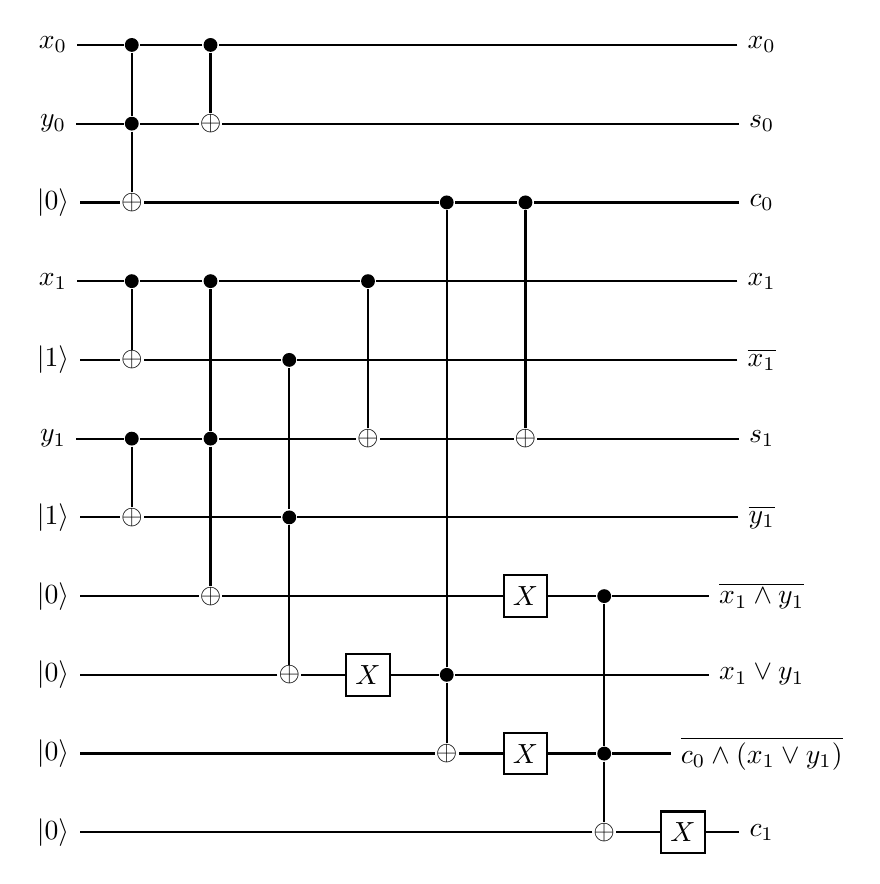
\begin{tikzpicture}[thick]
    %
    % `operator' will only be used by Hadamard (H) gates here.
    % `phase' is used for controlled phase gates (dots).
    % `surround' is used for the background box.
    \tikzstyle{operator} = [draw,fill=white,minimum size=1.5em] 
    \tikzstyle{phase} = [fill,shape=circle,minimum size=5pt,inner sep=0pt]
    \tikzstyle{surround} = [fill=blue!10,thick,draw=black,rounded corners=2mm]
    \tikzstyle{symbol} = [minimum size=5pt,inner sep=0pt]
    
    \node at (0,0) (begin1) {$x_0$};
    \node[phase] (p1) at (1,0) {} edge [-] (begin1);
    \node[phase] (p2) at (2,0) {} edge [-] (p1);
    \node at (9,0) (end1) {$x_0$} edge [-] (p2);

    \node at (0,-1) (begin2) {$y_0$};
    \node[phase] (p3) at (1,-1) {} edge [-] (begin2);
    \node[symbol](s1) at (2,-1) {$\oplus$} edge [-] (p3);
    \node at (9,-1) (end2) {$s_0$} edge [-] (s1);
    
    \node at (0,-2) (begin3) {$\ket{0}$};
    \node[symbol](s2) at (1,-2) {$\oplus$} edge [-] (begin3);
    \node[phase] (p4) at (5,-2) {} edge [-] (s2);
    \node[phase] (p5) at (6,-2) {} edge [-] (p4);
    \node at (9,-2) (end3) {$c_0$} edge [-] (p5);
    \draw[-] (p1) -- (p3);
    \draw[-] (p3) -- (s2);
    \draw[-] (p2) -- (s1);
    
    
    \node at (0,-3) (begin4) {$x_1$};
    \node[phase] (p6) at (1,-3) {} edge [-] (begin4);
    \node[phase] (p7) at (2,-3) {} edge [-] (p6);
    \node[phase] (p8) at (4,-3) {} edge [-] (p7);
    \node at (9,-3) (end4) {$x_1$} edge [-] (p8);
    
    
    \node at (0,-4) (begin5) {$\ket{1}$};
    \node[symbol](s3) at (1,-4) {$\oplus$} edge [-] (begin5);
    \node[phase] (p9) at (3,-4) {} edge [-] (s3);
    \node at (9,-4) (end5) {$\overline{x_1}$} edge [-] (p9);
    \draw[-] (p6) -- (s3);
    
    
    \node at (0,-5) (begin6) {$y_1$};
    \node[phase] (p10) at (1,-5) {} edge [-] (begin6);
    \node[phase] (p11) at (2,-5) {} edge [-] (p10);
    \node[symbol](s4) at (4,-5) {$\oplus$} edge [-] (p11);
    \node[symbol](s5) at (6,-5) {$\oplus$} edge [-] (s4);
    \node at (9,-5) (end6) {$s_1$} edge [-] (s5);
    \draw[-] (p8) -- (s4);
    \draw[-] (p5) -- (s5);
    
    \node at (0,-6) (begin7) {$\ket{1}$};
    \node[symbol](s6) at (1,-6) {$\oplus$} edge [-] (begin7);
    \node[phase] (p12) at (3,-6) {} edge [-] (s6);
    \node at (9,-6) (end7) {$\overline{y_1}$} edge [-] (p12);
    \draw[-] (p10) -- (s6);
    
    \node at (0,-7) (begin8) {$\ket{0}$};
    \node[symbol](s7) at (2,-7) {$\oplus$} edge [-] (begin8);
    \node[operator] (op1) at (6,-7) {$X$} edge [-] (s7);
    \node[phase] (p13) at (7,-7) {} edge [-] (op1);
    \node at (9,-7) (end8) {$\overline{x_1\wedge y_1}$} edge [-] (p13);
    \draw[-] (p7) -- (p11);
    \draw[-] (p11) -- (s7);
    
    \node at (0,-8) (begin9) {$\ket{0}$};
    \node[symbol](s8) at (3,-8) {$\oplus$} edge [-] (begin9);
    \node[operator] (op2) at (4,-8) {$X$} edge [-] (s8);
    \node[phase] (p14) at (5,-8) {} edge [-] (op2);
    \node at (9,-8) (end9) {$x_1\vee y_1$} edge [-] (p14);
    \draw[-] (p9) -- (p12);
    \draw[-] (p12) -- (s8);
    
    \node at (0,-9) (begin10) {$\ket{0}$};
    \node[symbol](s9) at (5,-9) {$\oplus$} edge [-] (begin10);
    \node[operator] (op3) at (6,-9) {$X$} edge [-] (s9);
    \node[phase] (p15) at (7,-9) {} edge [-] (op3);
    \node at (9,-9) (end10) {$\overline{c_0\wedge (x_1\vee y_1)}$} edge [-] (p15);
    \draw[-] (p4) -- (p14);
    \draw[-] (p14) -- (s9);
    
    \node at (0,-10) (begin11) {$\ket{0}$};
    \node[symbol](s10) at (7,-10) {$\oplus$} edge [-] (begin11);
    \node[operator] (op4) at (8,-10) {$X$} edge [-] (s10);
    \node at (9,-10) (end11) {$c_1$} edge [-] (op4);
    \draw[-] (p13) -- (p15);
    \draw[-] (p15) -- (s10);
    

    

\end{tikzpicture}


\item For $f=00$, there is no flipping of the lower bit, so that output equals the input, in which case we have 
\[U_{00} = I.\]
On the other hand, if $f=01$, then the lower bit is flipped only if the upper bit equals 1. But this is equivalent to a controlled-not gate.
Thus,
\[U_{01} = 
\left(\begin{array}{c|c}
I & \\
\hline
 &  X \\
\end{array}\right).\]
Finally, if $f=11$, then the lower bit is alwyas flipped, which corresponds with the matrix
\[
 U_{11} = 
\left(\begin{array}{c|c}
X & \\
\hline
 &  X \\
\end{array}\right).
\]
This is true since $U_{11}\ket{00} = \ket{01}$, $U_{11}\ket{01} = \ket{00}$, $U_{11}\ket{10} = \ket{11}$, and $U_{11}\ket{11} = \ket{10}$.

\item 
Let $A$ be a matrix whose columns form a permutation of the basis state vectors. Then $A$'s columns form an orthonormal basis. 
Moreover, $(A^{\dagger}A)_{ij}$ is the result of taking the dot product of column $i$ with column $j$, which, by orthonormality, is equal to 1 if $i=j$, and 0 otherwise.
In other words, $A^{\dagger}A= I$, and so $A$ is unitary.



\item We have
\[(U\otimes U)^{\dagger}(U\otimes U) = (U^{\dagger}\otimes U^{\dagger})(U\otimes U) = (U^{\dagger}U)\otimes (U^{\dagger}U) =\]
\[I_{n}\otimes I_n = I_{n^2},\]
where the 2nd equality is due to Theorem 5.
Therefore, by definition, $U\otimes U$ is unitary.


\item The signatures are expressed as the following $8\times 8$ matrix where, e.g., row 0 is $H_3\ket{000} =\ket{+++}$.

\[
\left(\begin{array}{cccccccc}
1 & 1 & 1 & 1 & 1 & 1 & 1 & 1\\
1 & -1 & 1 & -1 & 1 & -1 & 1 & -1\\
1 & 1 & -1 & -1 & 1 & 1 & -1 & -1\\
1 & -1 & -1 & 1 & 1 & -1 & -1 & 1\\
1 & 1 & 1 & 1 & -1 & -1 & -1 & -1\\
1 & -1 & 1 & -1 & -1 & 1 & -1 & 1\\
1 & 1 & -1 & -1 & -1 & -1 & 1 & 1\\
1 & -1 & -1 & 1 & -1 & 1 & 1 & -1\\
\end{array}\right)
\]






\item We have the following.

\begin{enumerate}
\item $(1,0,0) = 2/3\vec{v}_1 + 2/3\vec{v}_2 + 1/3\vec{v}_3$
\item $(-1,1,-2) = -2\vec{v}_1 + 1\vec{v}_2 - 1\vec{v}_3$
\item $(-3,5,1) = -3\vec{v}_1  - 1\vec{v}_2 + 3\vec{v}_3$
\end{enumerate}


\item Vectors $\vec{v}_2$ and $\vec{v}_3$ are not orthogonal.
 
\item Suppose $a=1$. If $b$ and $c$ have odd parity, then $a\cdot (b\oplus c)=1$ and 
 $a\cdot b \oplus a\cdot c = 1$, since $b=1$, or $c=1$, but not both. Now suppose $a=0$.
 Then 
 \[a\cdot (b\oplus c)= a\cdot b \oplus a\cdot c = 0.\]


\item Euclid's algorthm repeatedly uses the fact that, if $a=bq + r$, then  $\mbox{gcd}(a,b)=\mbox{gcd}(b,r)$. The algorithm stops when a remainder of $r=0$ is encountered.
\begin{enumerate}
\item We have
\[\mbox{gcd}(111,36) = \mbox{gcd}(36,3) = \mbox{gcd}(3,0) = 3.\]

\item We have
\[\mbox{gcd}(127,52) = \mbox{gcd}(52,23) = \mbox{gcd}(23,6) = \mbox{gcd}(6,5) = \mbox{gcd}(5,1) = \mbox{gcd}(1,0)  = 1.\]


\item We have
\[\mbox{gcd}(82,26) = \mbox{gcd}(26,4) = \mbox{gcd}(4,2) = \mbox{gcd}(2,0) = 2.\]
\end{enumerate}

\item The numbers 5, 7, 11, 13, and 17 are all relatively prime with 18. Their respective periods are 6, 3, 6, 3, 2.
For example, $17^2-1 = (18)(16)$, and so 17 has period equal to 2.


\item If $a^r=0\mbox{ mod } N$, then this implies that $N$ divides $a^r$, and so $a$ must share common prime factors with $N$, which contradicts
$\mbox{gcd}(a,N)=1$.

\item Assume $\mbox{gcd}(a,N)=1$,
The proof uses the fact that, if $a=b\mbox{ mod } N$, and $c$ divides both $a$ and $b$, but is relatively prime with $N$, then necessarily
\[\frac{a}{c}=\frac{b}{c}\mbox{ mod } N.\]
Now suppose there is no  $r\in\{1,\ldots,N-1\}$ for which $a^r=1\mbox{ mod }N$. 
Then by the previous exercise and the pigeion-hold principle, two of the following $N-1$ values 
\[a^1, a^2,\ldots,a^{N-1}\]
must be equal modulo $N$.
This is true since there are only $N-2$ possible values (namely $2,3,\ldots,N-1$)  that these values can assume. Hence, two of them must be equal.
Thus, suppose we have $a^r=a^s\mbox{ mod } N$ with $r > s$. Then since $\mbox{gcd}(a,N)=1$,
it follows that
\[a^{r-s}=1\mbox{ mod } N,\]
which is a contradiction. Therefore, there must exist at least one $r$ for which $a^r=1\mbox{ mod }N$.


\item Since 18 has exactly two prime factors, $s=2$, and we must show that at least $1-\frac{1}{2^{s-1}}=1/2$ of the periods $r$ have the property of being even,
and for which either $a^{r/2}-1$ or $a^{r/2}+1$ is not divisible by 18, and shares a factor with 18. This is true for the periods
of $a=5,11,17$, which gives a probability of $0.6 > 0.5$.


\item We have the following.
\begin{enumerate}
\item $18/25$ has convergents $1,2/3.3/4,5/7$.
\item $31/73$ has convergents $1/2,2/5,3/7,14/33$.
\item $15/38$ has convergents $1/2,1/3,2/5$.
\end{enumerate}

\item We have

\[F_3 = 2^{-3/2}
\left(\begin{array}{cccccccc}
1 & 1 & 1 & 1 & 1 & 1 & 1 & 1\\
1 & \frac{\sqrt{2}}{2}+ \frac{\sqrt{2}i}{2} & i & \frac{-\sqrt{2}}{2}+ \frac{\sqrt{2}i}{2} & -1 & \frac{-\sqrt{2}}{2}+ \frac{-\sqrt{2}i}{2} & -i & \frac{\sqrt{2}}{2}+ \frac{-\sqrt{2}i}{2}\\
1 & i & -1 & -i & 1 & i & -1 & -i\\
1 & \frac{-\sqrt{2}}{2}+ \frac{\sqrt{2}i}{2} & -i & \frac{\sqrt{2}}{2}+ \frac{\sqrt{2}i}{2} & -1 & \frac{\sqrt{2}}{2}+ \frac{-\sqrt{2}i}{2} & i & \frac{-\sqrt{2}}{2}+ \frac{-\sqrt{2}i}{2}\\
1 & -1 & 1 & -1 & 1 & -1 & 1 & -1\\
1 & \frac{-\sqrt{2}}{2}+ \frac{-\sqrt{2}i}{2} & i & \frac{\sqrt{2}}{2}+ \frac{-\sqrt{2}i}{2} & -1 & \frac{\sqrt{2}}{2}+ \frac{\sqrt{2}i}{2} & -i & \frac{-\sqrt{2}}{2}+ \frac{\sqrt{2}i}{2}\\
1 & -i & -1 & i & 1 & -i & -1 & i\\
1 & \frac{\sqrt{2}}{2}+ \frac{-\sqrt{2}i}{2} & -i & \frac{-\sqrt{2}}{2}+ \frac{-\sqrt{2}i}{2} & -1 & \frac{-\sqrt{2}}{2}+ \frac{\sqrt{2}i}{2} & i & \frac{\sqrt{2}}{2}+ \frac{\sqrt{2}i}{2}\\
\end{array}\right).
\]
Also, $F_3^{-1}=F_3^{\dagger}$.


\item The transformation is unitary since the fnction $f(y) = ay\mbox{ mod } N$ is a one-to-one correspondence over the set $\{0,1,\ldots,N-1\}$.
Moreover, for $k=1,\ldots,n$, we have
\[U_a\ket{u_k} = r^{-1/2}\sum_{j=0}^{r-1}e^{-\frac{2\pi ikj}{r}}\ket{a^{j+1}\mbox{ mod } N} = \]
\[(r^{-1/2})(e^{2\pi i\frac{k}{r}})\sum_{j=0}^{r-1}e^{-\frac{2\pi ik(j+1)}{r}}\ket{a^{j+1}\mbox{ mod } N} = (e^{2\pi i\frac{k}{r}})\ket{u_k}.\]
The last equality is true since the summation
\[ \sum_{j=0}^{r-1}e^{-\frac{2\pi ik(j+1)}{r}}\ket{a^{j+1}\mbox{ mod } N}\]
has the same terms as the original summation 
\[\sum_{j=0}^{r-1}e^{-\frac{2\pi ikj}{r}}\ket{a^j\mbox{ mod } N}.\]
To see this, it is an exercise to show that the $j$~th term of the former is equal to the $(j+1)$-term of the latter, while the $(j-1)$-term of the former is equal
to the zeroth term of the latter.


\item  Using the geometric series formula
\[\overset{n-1}{\underset{k=0}{\sum}}a^{k}=\frac{a^{n}-1}{a-1},\]
we have
\[\overset{n-1}{\underset{k=0}{\sum}}(\omega_{n}^{j})^{k}=\overset{n-1}{\underset{k=0}{\sum}}\omega_{n}^{jk}=\]
\[\frac{\omega_{n}^{jn}-1}{\omega_{n}^{j}-1}=\frac{\omega_{1}^{j}-1}{\omega_{n}^{j}-1}=\frac{1-1}{\omega_{n}^{j}-1}=0,\]
where the first equality is due to the cancellation rule, and the 2nd to last equality is due to the fact that $\omega_{1}^{1}=1$. Notice also
that the denominator is not equal to zero, since we assumed $j$ is not divisible by $n$; i.e. $j\not\equiv 0\mbox{ mod }n$.



\item We have
\[r^{-1/2}\sum_{k=1}^r\ket{u_k} = r^{-1/2}\sum_{k=1}^r (r^{-1/2}\sum_{j=0}^{r-1}e^{-\frac{2\pi ikj}{r}}\ket{a^j\mbox{ mod } N}) = \]
\[r^{-1}\sum_{j=0}^{r-1}(\sum_{k=1}^r e^{-\frac{2\pi ikj}{r}})\ket{a^j\mbox{ mod } N} = r^{-1}r\ket{1}=\ket{1},\]
where the second-to-last equality comes from the fact that, for $j\not= 0$,
\[\sum_{k=1}^r e^{-\frac{2\pi ikj}{r}} = 0\]
by the previous exercise. And for $j=0$,
\[\sum_{k=1}^r e^{-\frac{2\pi ik0}{r}} = \sum_{k=1}^r 1 = r.\]


\item 

\item 




\end{enumerate}

\end{document}

\section*{Extra Problems}

\begin{enumerate}

\item Let $\vec{e}_i$, $i=1,\ldots,n$, denote the column vector whose $i$~th component equals 1, and whose other components are zero.
Let $A$ be an $n\times n$ matrix whose $i$~the column is $\vec{e}_{\sigma(i)}$, where $\sigma$ is a permutation of the numbers $1,2,\ldots,n$.
In other words, the columns of $A$ constitute a re-ordering of $\vec{e}_1,\ldots,\vec{e}_n$. 
Show that $A$ is unitary. 



\end{enumerate}

%\end{document}


	
